% ------------------------------------------------------------------------------
% Formatvorlage für Masterarbeiten an der Ohm-Hochschule Nürnberg
% ------------------------------------------------------------------------------
%   erstellt von Stefan Macke, 24.04.2009
%   http://blog.stefan-macke.de

% Dokumentenkopf ---------------------------------------------------------------
%   Diese Vorlage basiert auf "scrreprt" aus dem koma-script.
% ------------------------------------------------------------------------------
\documentclass[
    11pt, % Schriftgröße
    DIV=11,
    ngerman, % für Umlaute, Silbentrennung etc.
    a4paper, % Papierformat
    twoside, % zweiseitiges Dokument
    titlepage, % es wird eine Titelseite verwendet
    parskip=half, % Abstand zwischen Abstüzen (halbe Zeile)
    headings=normal, % Größe der Überschriften verkleinern
    listof=totoc, % Verzeichnisse im Inhaltsverzeichnis aufführen
    bibliography=totoc, % Literaturverzeichnis im Inhaltsverzeichnis aufführen
    index=totoc, % Index im Inhaltsverzeichnis aufführen
    captions=tableheading, % Beschriftung von Tabellen unterhalb ausgeben
    final % Status des Dokuments (final/draft)
]{scrreprt}

% Meta-Informationen -----------------------------------------------------------
%   Informationen über das Dokument, wie z.B. Titel, Autor, Matrikelnr. etc
%   werden in der Datei Meta.tex definiert und können danach global
%   verwendet werden.
% ------------------------------------------------------------------------------
% Meta-Informationen -----------------------------------------------------------
%   Definition von globalen Parametern, die im gesamten Dokument verwendet
%   werden k�nnen (z.B auf dem Deckblatt etc.).
%
%   ACHTUNG: Wenn die Texte Umlaute oder ein Esszet enthalten, muss der folgende
%            Befehl bereits an dieser Stelle aktiviert werden:
%            \usepackage[latin1]{inputenc}
% ------------------------------------------------------------------------------
\newcommand{\titel}{Implementierung und Bewertung eines Konzeptes zum "Content
					  Relevance-Oriented Data Transport (CRODT)" \"uber Interplanetary
					  Communication Networks}
\newcommand{\untertitel}{und hier kommt der Untertitel}
\newcommand{\art}{Projektarbeit}
\newcommand{\fachgebiet}{Software-Engineering}
\newcommand{\autor}{Marian Haescher, Florian Ludwig, Philip Grunert}
\newcommand{\studienbereich}{}
\newcommand{\matrikelnrFLORIAN}{12 34 56}
\newcommand{\matrikelnrMARIAN}{12 34 56}
\newcommand{\matrikelnrPHILIP}{7200626}
\newcommand{\erstgutachter}{Prof. Dr.-Ing. habil. Djamshid Tavangarian}
\newcommand{\zweitgutachterA}{Dr.-Ing. Robil Daher}
\newcommand{\zweitgutachterB}{Mario Donick, M.A.}
\newcommand{\jahr}{2012}
\newcommand{\ort}{Rostock}
\newcommand{\logo}{UNI-Logo.pdf}


% benötigte Packages -----------------------------------------------------------
%   LaTeX-Packages, die benötigt werden, sind in die Datei Packages.tex
%   "ausgelagert", um diese Vorlage möglichst übersichtlich zu halten.
% ------------------------------------------------------------------------------
% Anpassung des Seitenlayouts --------------------------------------------------
%   siehe Seitenstil.tex
% ------------------------------------------------------------------------------
%\usepackage[
%    automark, % Kapitelangaben in Kopfzeile automatisch erstellen
%    headsepline, % Trennlinie unter Kopfzeile
%    ilines % Trennlinie linksbuendig ausrichten
%]{scrpage2}

% Anpassung an Landessprache ---------------------------------------------------
\usepackage[ngerman]{babel}

% Umlaute ----------------------------------------------------------------------
%   Umlaute/Sonderzeichen wie aeoeue direkt im Quelltext verwenden (CodePage).
%   Erlaubt automatische Trennung von Worten mit Umlauten.
% ------------------------------------------------------------------------------
\usepackage[utf8]{inputenc}
%\usepackage[T1]{fontenc}
\usepackage{textcomp} % Euro-Zeichen etc.

% Schrift ----------------------------------------------------------------------
\usepackage{lmodern} % bessere Fonts
\usepackage{relsize} % Schriftgroesse relativ festlegen
 
% Grafiken ---------------------------------------------------------------------
% Einbinden von JPG-Grafiken ermoeglichen
\usepackage[pdftex]{graphicx}
%Möglichkeit des Einfügens von Subfigures um Bilder nebeneinander einzufügen
\usepackage{subfigure}
% hier liegen die Bilder des Dokuments
\graphicspath{{Bilder/}}
% zum richtigen Positionieren der Bilder
\usepackage{float}
% zum seitenfüllenden Einfügen von PDFs und JPGs
\usepackage{pdfpages}

% Befehle aus AMSTeX f�r mathematische Symbole z.B. \boldsymbol \mathbb --------
\usepackage{amsmath,amsfonts}

% f�r Index-Ausgabe mit \printindex --------------------------------------------
\usepackage{makeidx}

% Einfache Definition der Zeilenabstaende und Seitenraender etc.
% -----------------
\usepackage{setspace}
\usepackage{geometry}

% glossar/Symbolverzeichnis
% ------------------------------------------------------------   Symbolverzeichnisse bequem erstellen. Beruht auf MakeIndex:
%     makeindex.exe %Name%.nlo -s nomencl.ist -o %Name%.nls
%   erzeugt dann das Verzeichnis. Dieser Befehl kann z.B. im TeXnicCenter
%   als Postprozessor eingetragen werden, damit er nicht staendig manuell
%   ausgefuehrt werden muss.
%   Die Definitionen sind ausgegliedert in die Datei "Glossar.tex".
% ------------------------------------------------------------------------------
%Paket laden 
\usepackage[
nonumberlist, %keine Seitenzahlen anzeigen
acronym,      %ein Abkürzungsverzeichnis erstellen
toc]          %Einträge im Inhaltsverzeichnis
{glossaries}


% zum Umfliessen von Bildern
% ----------------------------------------------------
\usepackage{floatflt}


% zum Einbinden von Programmcode -----------------------------------------------
\usepackage{listings}
\usepackage{xcolor} 
\definecolor{hellgelb}{rgb}{1,1,0.9}
\definecolor{colKeys}{rgb}{0,0,1}
\definecolor{colIdentifier}{rgb}{0,0,0}
\definecolor{colComments}{rgb}{1,0,0}
\definecolor{colString}{rgb}{0,0.5,0}
\lstset{
    float=hbp,
    basicstyle=\ttfamily\color{black}\small\smaller,
    identifierstyle=\color{colIdentifier},
    keywordstyle=\color{colKeys},
    stringstyle=\color{colString},
    commentstyle=\color{colComments},
    columns=flexible,
    tabsize=2,
    frame=single,
    extendedchars=true,
    showspaces=false,
    showstringspaces=false,
    numbers=left,
    numberstyle=\tiny,
    breaklines=true,
    backgroundcolor=\color{hellgelb},
    breakautoindent=true
}
\lstset{literate=%
{Ö}{{\"O}}1
{Ä}{{\"A}}1
{Ü}{{\"U}}1
{ß}{{\ss}}2
{ü}{{\"u}}1
{ä}{{\"a}}1
{ö}{{\"o}}1
}

% URL verlinken, lange URLs umbrechen etc. -------------------------------------
\usepackage{url}

% wichtig f�r korrekte Zitierweise ---------------------------------------------
\usepackage[square]{natbib}

% PDF-Optionen -----------------------------------------------------------------
\usepackage[
    bookmarks,
    bookmarksopen=true,
    colorlinks=true,
% diese Farbdefinitionen zeichnen Links im PDF farblich aus
    linkcolor=black, % einfache interne Verknuepfungen
    anchorcolor=black,% Ankertext
    citecolor=blue, % Verweise auf Literaturverzeichniseintraege im Text
    filecolor=magenta, % Verknuepfungen, die lokale Dateien oeffnen
    menucolor=red, % Acrobat-Menuepunkte
    urlcolor=cyan, 
% diese Farbdefinitionen sollten fuer den Druck verwendet werden (alles schwarz)
    %linkcolor=black, % einfache interne Verknuepfungen
    %anchorcolor=black, % Ankertext
    %citecolor=black, % Verweise auf Literaturverzeichniseintraege im Text
    %filecolor=black, % Verknuepfungen, die lokale Dateien oeffnen
    %menucolor=black, % Acrobat-Men�punkte
    %urlcolor=black, 
    backref,
    plainpages=false, % zur korrekten Erstellung der Bookmarks
    pdfpagelabels, % zur korrekten Erstellung der Bookmarks
    hypertexnames=false, % zur korrekten Erstellung der Bookmarks
    %linktocpage % Seitenzahlen anstatt Text im Inhaltsverzeichnis verlinken
]{hyperref}
% Befehle, die Umlaute ausgeben, f�hren zu Fehlern, wenn sie hyperref als
% Optionen uebergeben werden
\hypersetup{
    pdftitle={\titel \untertitel},
    pdfauthor={\autor},
    pdfcreator={\autor},
    pdfsubject={\titel \untertitel},
    pdfkeywords={\titel \untertitel},
}

% fortlaufendes Durchnummerieren der Fussnoten
% ----------------------------------
\usepackage{chngcntr}

% f�r (lange) Tabellen ---------------------------------------------------------
\usepackage{longtable}
\usepackage{array}
\usepackage{ragged2e}
\usepackage{lscape}
\usepackage{tabularx}

% Spaltendefinition rechtsbuendig mit definierter Breite
% ------------------------
\newcolumntype{w}[1]{>{\raggedleft\hspace{0pt}}p{#1}}

% Formatierung von Listen aendern
% -----------------------------------------------
\usepackage{paralist}

% bei der Definition eigener Befehle benoetigt
\usepackage{ifthen}

% definiert u.a. die Befehle \todo und \listoftodos
\usepackage{todonotes}

% sorgt daf�r, dass Leerzeichen hinter parameterlosen Makros nicht als Makroendezeichen interpretiert werden
\usepackage{xspace}

\usepackage{fancyhdr}
\raggedbottom

%  Latex wird sich bemühen, immer im Blocksatz zu bleiben, auch wenn dadurch große Abstände zwischen Wörtern entstehen
\sloppy

% Erstellung eines Index und Abkürzungsverzeichnisses aktivieren ---------------
\makeindex
%\makenomenclature

% Kopf- und Fußzeilen, Seitenränder etc. ---------------------------------------
% Zeilenabstand 1,5 Zeilen -----------------------------------------------------
\onehalfspacing

% Seitenraender
% -----------------------------------------------------------------
\setlength{\topskip}{\ht\strutbox} % behebt Warnung von geometry
\geometry{paper=a4paper,left=35mm,right=35mm,top=30mm} % Ohne Binderand

\geometry{a4paper,inner=3.5cm,outer=2.5cm,top=2.5cm,bottom=2.5cm,pdftex} % Mit
% Binderand


% Kopf- und Fußzeilen ----------------------------------------------------------
\pagestyle{fancy} %scrheadings
% Kopf- und Fußzeile auch auf Kapitelanfangsseiten

\renewcommand*{\chapterpagestyle}{fancy}

%\renewcommand{\chapterpagestyle}{fancy} 
% Schriftform der Kopfzeile
\renewcommand{\headfont}{\normalfont}

\fancyhead[ER]{\nouppercase{\sc\leftmark}}
\fancyhead[EL]{\nouppercase{\sc\rightmark}}
\fancyhead[OR]{\nouppercase{\sc\rightmark}}
\fancyhead[OL]{\nouppercase{\sc\leftmark}}





%\renewcommand{\sectionmark}[1]{\markboth{#1}{}}


% Kopfzeile
\ihead{\textit{\headmark}}
\chead{}
\ohead{\pagemark}

% Fußzeile
\ifoot{\copyright\ \autor}
\cfoot{}
\ofoot{}

% sonstige typographische Einstellungen ----------------------------------------

% erzeugt ein wenig mehr Platz hinter einem Punkt
\frenchspacing 

% Schusterjungen und Hurenkinder vermeiden
\clubpenalty = 10000
\widowpenalty = 10000 
\displaywidowpenalty = 10000

% Quellcode-Ausgabe formatieren
\lstset{numbers=left, numberstyle=\tiny, numbersep=5pt, breaklines=true}
\lstset{emph={square}, emphstyle=\color{red}, emph={[2]root,base}, emphstyle={[2]\color{blue}}}

% Fußnoten fortlaufend durchnummerieren
\counterwithout{footnote}{chapter}


% eigene Definitionen für Silbentrennung
% Trennvorschl�ge im Text werden mit \" angegeben
% untrennbare W�rter und Ausnahmen von der normalen Trennung k�nnen in dieser
% Datei mittels \hyphenation definiert werden


% eigene LaTeX-Befehle
% Eigene Befehle und typographische Auszeichnungen für diese

% einfaches Wechseln der Schrift, z.B.: \changefont{cmss}{sbc}{n}
\newcommand{\changefont}[3]{\fontfamily{#1} \fontseries{#2} \fontshape{#3} \selectfont}

% Abk�rzungen mit korrektem Leerraum 
\newcommand{\ua}{\mbox{u.\,a.\ }}
\newcommand{\zB}{\mbox{z.\,B.\ }}
\newcommand{\dahe}{\mbox{d.\,h.\ }}
\newcommand{\Vgl}{Vgl.\ }
\newcommand{\bzw}{bzw.\ }
\newcommand{\evtl}{evtl.\ }
\newcommand{\ca}{ca.\ }
\newcommand{\etc}{etc.\ }

\newcommand{\abbildung}[1]{Abbildung~\ref{fig:#1}}

\newcommand{\bs}{$\backslash$}

% erzeugt ein Listenelement mit fetter Überschrift 
\newcommand{\itemd}[2]{\item{\textbf{#1}}\\{#2}}

% einige Befehle zum Zitieren --------------------------------------------------
\newcommand{\Zitat}[2][\empty]{\ifthenelse{\equal{#1}{\empty}}{\citep{#2}}{\citep[#1]{#2}}}

% zum Ausgeben von Autoren
\newcommand{\AutorName}[1]{\textsc{#1}}
\newcommand{\Autor}[1]{\AutorName{\citeauthor{#1}}}

% verschiedene Befehle um Wörter semantisch auszuzeichnen ----------------------
\newcommand{\NeuerBegriff}[1]{\textbf{#1}}
\newcommand{\Fachbegriff}[1]{\textit{#1}}

\newcommand{\Eingabe}[1]{\texttt{#1}}
\newcommand{\Code}[1]{\texttt{#1}}
\newcommand{\Datei}[1]{\texttt{#1}}

\newcommand{\Datentyp}[1]{\textsf{#1}}
\newcommand{\XMLElement}[1]{\textsf{#1}}
\newcommand{\Webservice}[1]{\textsf{#1}}


% ------------ glossar initialisieren -----
%Ein eigenes Symbolverzeichnis erstellen
\newglossary[slg]{symbolslist}{syi}{syg}{Symbolverzeichnis} 

%Den Punkt am Ende jeder Beschreibung deaktivieren
\renewcommand*{\glspostdescription}{}

%Glossar-Befehle anschalten
\makeglossaries
%Befehle für Abkürzungen
\newacronym{DOID}{DOID}{Data Object Identification Number}
\newacronym{FIFO}{FIFO}{First In First Out}
\newacronym{IF}{IF}{Interface}
\newacronym{STL}{STL}{Standard Template Library}
\newacronym{CRODM}{CRODM}{Content Relevance-oriented Data
 Management}
\newacronym{CROP}{CROP}{Content Relevance-Ortiented Prioritization}
\newacronym{ROTP}{ROTP}{Relevance-Ortiented Transport Protocol}
\newacronym{TCP}{TCP}{Transmission Control Protocol}
\newacronym{UDP}{UDP}{User Datagram Protocol}
\newacronym{DTN}{DTN}{Delay Tolerant Networks}
\newacronym{IPN}{IPN}{Interplanetary Internet}
\newacronym{CCSDS}{CCSDS}{Consultative Committee for Space Data Systems}
\newacronym{CFDP}{CFDP}{CCSDS File Delivery Protocol}
\newacronym{LTP}{LTP}{Licklider Transmission Protocol}
\newacronym{DSN}{DSN}{Deep Space Network}
\newacronym{TTL}{TTL}{Time To Live}
\newacronym{ASCII}{ASCII}{American Standard Code for Information Interchange}
\newacronym{IP}{IP}{Internet Protocol}
\newacronym{XML}{XML}{Extensible Markup Language}
\newacronym{CRODT}{CRODT}{Content Relevance-Oriented Data Transport}
\newacronym{GUI}{GUI}{Graphical User Interface}
\newacronym{QoS}{QoS}{Quality of Service}
\newacronym{QoI}{QoI}{Quality of Interaction}
\newacronym{CRC}{CRC}{Cyclic Redundancy Check}

%Befehle für Glossar
% \newglossaryentry{glos:Overlay}{
% name=Overlay,
% description={Overlay noch hinzufügen}
% }
% 
% \newglossaryentry{glos:Capricorn}{
% name=Capricorn,
% description={Steinbock}
% }
% 
% \newglossaryentry{glos:Aquarius}{
% name=Aquarius,
% description={Wassermann}
% }
% 
% \newglossaryentry{glos:Pisces}{
% name=Pisces,
% description={Fische}
% }
% 
% \newglossaryentry{glos:Aries}{
% name=Aries,
% description={Widder}
% }
% 
% \newglossaryentry{glos:Taurus}{
% name=Taurus,
% description={Stier}
% }
% 
% \newglossaryentry{glos:Gemini}{
% name=Gemini,
% description={Zwillinge}
% }
% 
% \newglossaryentry{glos:Cancer}{
% name=Cancer,
% description={Krebs}
% }
% 
% \newglossaryentry{glos:Leo}{
% name=Leo,
% description={Löwe}
% }
% 
% \newglossaryentry{glos:Virgo}{
% name=Virgo,
% description={Jungfrau}
% }
% 
% \newglossaryentry{glos:Libra}{
% name=Libra,
% description={Waage}
% }
% 
% \newglossaryentry{glos:Scorpio}{
% name=Scorpio,
% description={Skorpion}
% }
% 
% \newglossaryentry{glos:Sagittarius}{
% name=Sagittarius,
% description={Schütze}
% }

% Befehle für Symbole
% \newglossaryentry{symb:Pi}{
% name=$\pi$,
% description={Die Kreiszahl.},
% sort=symbolpi, type=symbolslist
% }
% \newglossaryentry{symb:Phi}{
% name=$\varphi$,
% description={Ein beliebiger Winkel.},
% sort=symbolphi, type=symbolslist
% }
% \newglossaryentry{symb:Lambda}{
% name=$\lambda$,
% description={Eine beliebige Zahl, mit der der nachfolgende Ausdruck
% multipliziert wird.},
% sort=symbollambda, type=symbolslist
% }


% beispiel einer Abkürzung mit Glossareintrag
% \newacronym{AD}{AD}{Active Directory\protect\glsadd{glos:AD}}
% \newglossaryentry{glos:AntwD}{
% name=Antwortdatei,
% description={Informationen zum
% Installieren einer Anwendung oder des Betriebssystems.}
% }


% Das eigentliche Dokument -----------------------------------------------------
%   Der eigentliche Inhalt des Dokuments beginnt hier. Die einzelnen Seiten
%   und Kapitel werden in eigene Dateien ausgelagert und hier nur inkludiert.
% ------------------------------------------------------------------------------
\begin{document}

% auch subsubsection nummerieren
\setcounter{secnumdepth}{3}
\setcounter{tocdepth}{3}

% Deckblatt und Abstract ohne Seitenzahl
%!TEX root = ./Literaturarbeit.tex
% \begin{titlepage}
% 		\begin{center}
% 		
% 			\begin{figure}[H]
% 				\centering
% 				
\includegraphics[scale=.2]{Bilder/unirostock_logo.jpeg}
% 			\end{figure}
% 			\textbf{\large Universität Rostock\\}
% 			\vspace{1.5cm}
% 			\textbf{\large Fakultät für Informatik und Elektrotechnik\\}
% 			\vspace{0.2cm}
% 			\textbf{\large Institut für Automatisierungstechnik\\}
% 			\vspace{1.5cm}
% 			\textbf{\Large Bachelorarbeit\\}
% 			\vspace{1.5cm}
% 			\textbf{\large ``Modellbasierte Optimierung von Stellgrößentrajektorien\\}
% 			\vspace{0.2cm}
% 			\textbf{\large  in zyklisch arbeitenden Herzunterstützungssystemen unter\\}
% 			\vspace{0.2cm}
% 			\textbf{\large medizinischen und technischen Randbedingungen"\\}
% 			\vspace{3cm}
% 			
% 			\textbf{\centering
% 			\begin{tabularx}{400pt}{ll}
% 				Bearbeiter: & Philip Grunert\\
% 				Studiengang: & ITTI\\
% 				Matrikelnummer: & 7200626\\
% 				Bearbeitungszeitraum: & 01.06.2011 - 07.09.2011\\
% 				Betreuender Hochschullehrer: & Prof. Dr.-Ing. habil. Dr. h.c. Bernhard Lampe \\ 
% 				Betreuer: & M.Sc. Alexander Sievert \\
% 			\end{tabularx}
% 			}		
% 				
% 		\end{center}	
% 	\end{titlepage}

\thispagestyle{plain}
\begin{titlepage}

\begin{center}

\huge{\textbf{\titel}}\\[1.5ex]
\LARGE{\textbf{\art}}\\[1.5ex]
\Large{im Fachgebiet \fachgebiet}\\[15ex]

\includegraphics[scale=0.2]{\logo}\\[6ex]

\normalsize
\begin{tabular}{w{5.4cm}p{6cm}}\\
vorgelegt von:  & \quad Marian Haescher\\[1.2ex]
				& \quad Florian Ludwig\\[1.2ex]
				& \quad Philip Grunert\\[1.2ex]
Studiengang: 	& \quad Informationstechnik/Technische\\[1.2ex]
			 	& \quad Informatik\\[1.2ex]
Matrikelnummer: & \quad \matrikelnrFLORIAN\\[1.2ex]
Erstgutachter:  & \quad \erstgutachter\\[1.2ex]
Zweitgutachter: & \quad \zweitgutachter\\[3ex]
\end{tabular}

\copyright\ \jahr\\[9ex]

\end{center}

\singlespacing
\small
\noindent Dieses Werk einschließlich seiner Teile ist \textbf{urheberrechtlich geschützt}. Jede Verwertung außerhalb der engen Grenzen des Urheberrechtgesetzes ist ohne Zustimmung des Autors unzulässig und strafbar. Das gilt insbesondere für Vervielfältigungen, Übersetzungen, Mikroverfilmungen sowie die Einspeicherung und Verarbeitung in elektronischen Systemen.

\end{titlepage} 

% Aufgabenstellung
\cleardoublepage
\thispagestyle{empty}
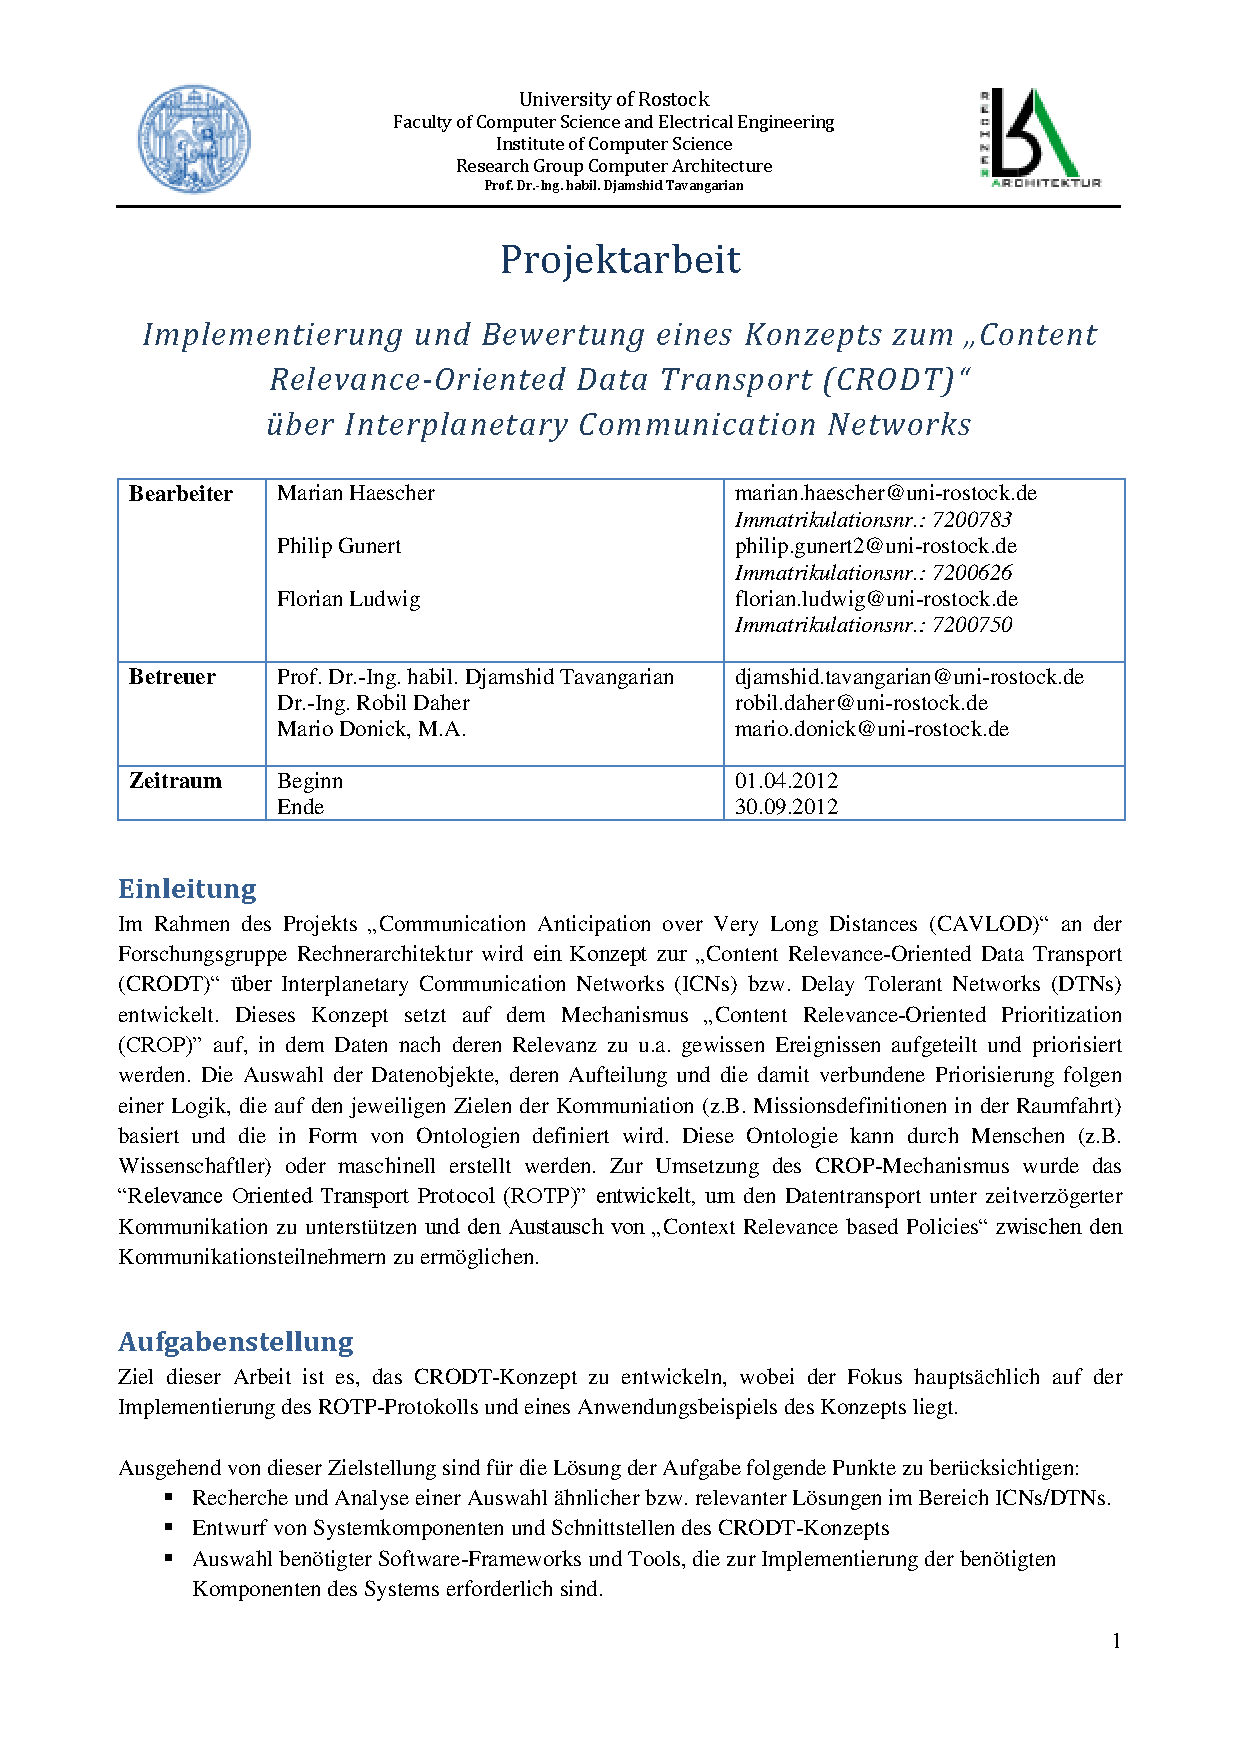
\includepdf[pages=-]{Aufgabenstellung.pdf}

% Seitennummerierung -----------------------------------------------------------
%   Vor dem Hauptteil werden die Seiten in großen römischen Ziffern 
%   nummeriert.
% ------------------------------------------------------------------------------


\pagenumbering{Roman}
\tableofcontents % Inhaltsverzeichnis

% Abkürzungsverzeichnis
% --------------------------------------------------------
% % für eine korrekte Überschrift in der Kopfzeile
\clearpage
 
%Glossar ausgeben
\printglossary[style=altlist,title=Glossar]

%Abkürzungen ausgeben
\deftranslation[to=German]{Acronyms}{Abkürzungsverzeichnis}
\printglossary[type=\acronymtype,style=long,title=Abkürzungsverzeichnis]

%Symbole ausgeben
\printglossary[type=symbolslist,style=long,title=Symbolverzeichnis]
 

\listoffigures % Abbildungsverzeichnis
\listoftables % Tabellenverzeichnis
\renewcommand{\lstlistlistingname}{Verzeichnis der Listings}
\lstlistoflistings % Listings-Verzeichnis

% arabische Seitenzahlen im Hauptteil ------------------------------------------
%\clearpage
\cleardoublepage
\pagenumbering{arabic}


% die Inhaltskapitel werden in "Inhalt.tex" inkludiert -------------------------

\chapter{Einleitung}
	\section{Motivation}

Seit {\"u}ber f{\"u}nfzig Jahren entwickeln Forscher Strategien
zur Erkundung des Weltraums. Dabei hat sich seit der Entsendung des ersten k{\"u}nstlichen
Satelliten namens Sputnik und der ersten Mondlandung viel getan.
Zahlreiche Sonden oder Landefahrzeuge wurden seither zu diversen Zielen unseres
Sonnensystems entsandt, um neue Erkenntnisse {\"u}ber unser Universum und dessen
Entstehung zu sammeln. Ein aktuelles Beispiel stellt der Mars Rover Curiosity
dar, welcher j{\"u}ngst im Gale Krater auf dem Mars landete. Der Rover
verf{\"u}gt {\"u}ber zahlreiche Messinstrumente, darunter Kameras, Sensoren zur
Messung kosmischer Strahlung, Spektrografen, meteorologische Messinstrumente und
vieles mehr. Der Rover selbst ist mit einem Gewicht von $900$ kg und der
Gr{\"o}{\ss}e eines kompakten Kleinwagens das bisher mit Abstand gr{\"o}{\ss}te
vom Menschen geschaffene Objekt, das je die Marsoberfl{\"a}che erreichte.
\textit{Curiosity} stellt ein mobiles Labor dar, das neben den Sensoren und
Messinstrumenten auch Greifarme und R{\"a}der zur Fortbewegung und Interaktion
aufweist. Alle Messinstrumente und s{\"a}mtliche Peripherie des Rovers werden dabei von der
Erde aus gesteuert. \newline
Mit steigender Komplexit{\"a}t der mobilen Labore
steigt nat{\"u}rlich auch die Menge an Daten, die es zu {\"u}bertragen gilt. Da
die komplette Steuerung und Auswertung auf der Erde stattfindet, gilt es, sowohl
Steuerdaten von der Erde an den Rover zu senden, als auch Messdaten, Bilder und
{\"a}hnliches vom Rover an die Erde zu {\"u}bermitteln. Dabei unterliegt die
Kommunikation einigen entscheidenden Restriktionen. Die wohl Wichtigste ist die
Lichtgeschwindigkeit, welche sich im Vakuum mit $299 792 458$ m/s ausbreitet.
Die Ausbreitung der entsandten Signale kann daher niemals schneller erfolgen. Da die
Entfernung zum Mars je nach Konstellation (Position der Planeten zueinander,
w{\"a}hrend ihrer Bewegung um die Sonne) variiert, ist es im Folgenden
hilfreich, von der mittleren minimalen Entfernung zur Erde auszugehen. Diese betr{\"a}gt $0,52$ AE oder aber ca. $77,8$ Millionen Kilometer (Schwankung des
$[Erde - Mars]$ Abstandes je nach Konstellation: $0,372 - 2,683$ AE, d.h. bei
Opposition $[Sonne - Erde - Mars]$ zwischen ca. $55 - 105$ Millionen Kilometern
und bei Konjunktion $[Mars - Sonne - Erde]$ ca. $400$ Millionen Kilometer).
Ausgehend von dieser Entfernung, bei einer Ausbreitungsgeschwindigkeit der
Signale von ca. $300.000$ km/s, erh{\"a}lt man eine Dauer von ca. $4,3$ Minuten
pro {\"U}bertragungsrichtung. Daraus folgt, dass die Antwort, auf eine an den
Mars gesandte Anfrage bei diesem Szenario im Idealfall nach $8,6$
Minuten, die Erde erreicht (im Fall der maximalen Entfernung zwischen Erde und
Mars erst nach $44$ Minuten, wobei in dieser Konstellation eine direkte
Funkverbindung nahezu unm{\"o}glich ist). Da der Mars jedoch genau wie die Erde
eine Rotation um seine eigene Achse ausf{\"u}hrt und die Kommunikation {\"u}ber eine den Mars
umkreisende Sendevorrichtung (Satellit) erfolgt, wird das Zeitfenster der
{\"U}bertragung weiter beschr{\"a}nkt (Zeitfenster betr{\"a}gt ca. 30 Minuten
pro Tag aufgeteilt in zwei Sendevorg{\"a}nge von je 15 Minuten, dies ist jeweils
die Zeit f{\"u}r den Vorbeiflug des Orbiters von Horizont zu Horizont bezogen
auf den Rover).\newline \newline
Diese physikalisch begr{\"u}ndeten Latenzen sind ein wichtiger Faktor, den es in
der interplanetaren Kommunikation zu ber{\"u}cksichtigen gilt. Die hieraus
abzuleitende Erkenntnis ist, dass eine Kommunikation beispielsweise zwischen
Erde und Mars nicht mit einer heutigen irdischen Kommunikation zu vergleichen
ist. Zwar ist das Modell der verz{\"o}gerten Kommunikation dem Menschen
keineswegs unbekannt.
Hier sei Exemplarisch auf den vor der Erfindung der Telegraphie
ausschlie{\ss}lich betriebenen Briefverkehr verwiesen. Jedoch ist dieses
Ph{\"a}nomen in der heutigen vernetzten Generation nahezu in Vergessenheit
geraten. Die irdische Kommunikation im $21$. Jahrhundert setzt auf geringe
Latenzen und kann somit idealisiert als verz{\"o}gerungsfrei betrachtet werden.
Doch eine interplanetare Kommunikation wird nicht allein durch die
unvermeidlichen Latenzen beeinflusst. Auch die Bandbreite unserer
{\"U}bertragung unterliegt der Erde abgewandten Seite einer Beschr{\"a}nkung. Am
Beispiel der Mars Rover sei hier auf die genutzten Solarpanele bzw. eingesetzten
Batterien (zumeist Radionuklidbatterien) verwiesen, welche nur eine begrenzte
Energieversorgung gew{\"a}hrleisten und somit keine nahezu unbegrenzte
Sendeleistung erm{\"o}glichen, wie es auf der Erde der Fall ist.\newline
Ein weiterer Punkt ist die f{\"u}r den Rover eingesetzte Technologie. Hierbei 
sind unter anderem Faktoren wie Gr{\"o}{\ss}e und Gewicht von Bedeutung, da 
diese die Kosten der Unternehmung stark beeinflussen. So kostet beispielsweise 
der Start einer Ariane $5$ Rakete zwischen $125$ und $155$ Millionen Euro bei 
einer Nutzlast von $23.000$ kg im LEO (Low Earth Orbit: $200-2.000$ km).
Hieraus ergibt sich f{\"u}r dieses Beispiel ein Preis von ca. $7.000$ Euro pro kg 
Nutzlast. An diesem Beispiel zeigt sich die Wichtigkeit einer genauen
Kalkulation des Gewichtes der Rover. Diese Restriktion wirkt sich direkt auf die
verbaute Hardware des Rovers aus und somit auch indirekt auf Ressourcen wie z.B.
die Gr{\"o}{\ss}e des verbauten Speichers zum Ablegen lokaler Daten.\newline
Zusammenfassend kann anhand der Beispiele festgestellt werden, dass Latenz, 
Bandbreite sowie lokaler Speicher wichtige Restriktionen sind, denen die 
interplanetare Kommunikation unterliegt. Diese Voraussetzungen verlangen 
eine besondere Kommunikationsstruktur die von den {\"u}blichen Protokollen 
abweicht. 

\section{Ziel der Arbeit}

Das \gls{CROP} soll bei den zuvor erw{\"a}hnten Sachverhalten f{\"u}r Abhilfe
sorgen. Der Gedanke des Protokolls ist ein gezielter Umgang mit den begrenzten 
Ressourcen. Hierbei wird einerseits eine Unterteilung der vorhandenen 
Daten in Datenbl{\"o}cke vorgenommen und andererseits eine Priorisierung der 
Daten erwirkt, welche {\"u}ber die Reihenfolge und den Zeitpunkt des 
Versendens entscheidet. Daraus resultiert, dass Daten von hoher Relevanz 
vor Daten niederer Relevanz verschickt werden. Somit k{\"o}nnen 
beispielsweise zeitkritische Daten das Kontrollzentrum auf der Erde 
schneller erreichen. Zudem hat das priorisierte Zerteilen der Daten
(priorisiertes Contentsplitting) den Vorteil, dass Daten gro{\ss}er
Speichermenge (z.B.
hochaufl{\"o}sende Bilder) bereits vor dem vollst{\"a}ndigen Empfang auf der
Erde partiell visualisiert und ausgewertet werden k{\"o}nnen. Das Ziel der
vorliegenden Arbeit ist die Implementation des \gls{CROP} und einer Anwendung
zur Nutzung dieses Protokolls (Chatanwendung). Zudem erfolgt eine Evaluierung
des implementierten Protokolls hinsichtlich der Performanz und Stabilit{\"a}t.
Au{\ss}erdem umfasst die Arbeit weiterf{\"u}hrende {\"U}berlegungen im Bezug auf
die zuk{\"u}nftige Weiterentwicklung des \gls{CROP}.

\section{Aufbau der Arbeit}

Im Folgenden wird ein kurzer {\"U}berblick zu den einzelnen
Kapiteln der Arbeit gew{\"a}hrt.

In \textbf{Kapitel zwei} werden die Grundlagen der Netzwerkkommunikation
aufgef{\"u}hrt, welche zum Verst{\"a}ndnis der Arbeit notwendig sind. Dabei wird
\zB das OSI-Referenzmodell aufgegriffen und erl{\"a}utert. Die im Weiteren
erl{\"a}uterten Modelle k{\"o}nnen alle vom OSI-Schichtenmodell abgeleitet
werden. Die weiteren Grundlagen betreffen die Zeitmessung auf dem Mars und
andere allgemeine Erl{\"a}uterungen.

Das \textbf{dritte Kapitel} befasst sich mit dem aktuellen Stand der Technik.
Hier werden aktuelle Technologien und Protokolle vorgestellt, welche in der
interplanetaren Kommunikation zum Einsatz kommen.

\textbf{Kapitel vier} umfasst das Konzept der Arbeit. Hier werden
Vor{\"u}berlegungen zur Entwicklung eines \gls{CROP} ausgef{\"u}hrt und
grundlegende Funktionen erl{\"a}utert, die dabei zum Einsatz kommen.
Zudem werden einige Ideen beleuchtet, welche in der weiteren
Protokollentwicklung zu ber{\"u}cksichtigen sind, die aber im derzeitigen Stand
nicht implementiert wurden.

\textbf{Kapitel f{\"u}nf} behandelt die Implementierung des Protokolls. Dabei
wird sowohl die Implementierung der betreffenden Module für das Protokoll
genauer er{\"o}rtert, als auch die Entwicklung der grafischen
Benutzeroberfläche f{\"u}r eine einfache Chat-Kommunikation.

Im \textbf{sechsten Kapitel} wird unsere Implementierung des Protokolls
hinsichtlich Overhead, Speicherverbrauch und Laufzeit analysiert und diskutiert.

Im \textbf{siebten und letzten Kapitel} werden eine Zusammenfassung und ein
Ausblick auf die zuk{\"u}nftige Entwicklung im bearbeiteten Themenbereich gegeben.



\chapter{Grundlagen}
	Diese Kapitel befasst sich mit den Grundlagen die zum Verst{\"a}ndnis der Arbeit
notwendig sind. Dies umfasst allgemeine Grundlagen im Bereich der
Netzwerktechnik sowie Themen von Wichtigkeit f{\"u}r eine Interplanetare Kommunikation.

	\section{Protokoll-Stack}
		Der Protocol Stack bzw. Protokollstapel bezeichnet die Verschachtelung der
einzelnen Schichten, die zur Erf{\"u}llung einer Protokollkommunikation
notwendig sind. Dabei werden die Daten der vorherigen Schicht zur
Weiterverarbeitung der nachfolgenden Schicht zugef{\"u}hrt. Dieses Stapelprinzip
gibt dem Protocol Stack seinen Namen. Der Stack {\"u}bernimmt dabei
s{\"a}mtliche Koordination und Verarbeitung der Datenstr{\"o}me (z.B.
Segmentierungen, Adressierung etc.).
Je nach Anforderung an die Kommunikation muss der Stack angepasst werden. Die
eingehenden Daten werden im Top-down Verfahren durch den Stack verpackt
und in einer FIFO (First-In-First-Out) gepuffert. Nach dem Versenden werden die
Daten auf der Empfangsseite durch das Bottom-up Verfahren wieder ausgepackt und k{\"o}nnen
ausgewertet werden.

	\section{OSI-Modell}
		Dieser Abschnitt befasst sich mit der Kommunikation zwischen dem Client
und dem Server (z.B. Station auf der Erde und Rover auf dem Mars). Die
Kommunikation erfolgt hierbei {\"u}ber UDP Sockets. Das im verlauf der Arbeit
Implementierte CROP Protokoll verpackt zuvor die Inhalte (Bilder, Sensordaten etc.) 
nach den Protokollvorgaben und reicht die Datenpakete aus der priorisierten Queue 
direkt an den zuvor ge{\"o}ffneten UDP Socket weiter. Durch eine Client/Server
basierte Socket-Kommunikation {\"u}ber UDP 
(verbindungslose Kommunikation im Gegensatz zu TCP) wird der Datenstrom an die
definierte Zieladresse und den definierten Zielport geleitet. Da es sich
hierbei um eine UDP Socket-Verbindung handelt, werden Paketverluste nicht
bemerkt (keine Sicherung der Daten{\"u}bertragung). Lediglich ein {\"u}bergreifendes
Protokoll wie CROP, welches dies erkennen k{\"o}nnte, kann dann eine erneute
Sendung anfordern (zum jetzigen Zeitpunkt ist CROP jedoch nicht f{\"a}hig einen
Verbindungsabbruch zu detektieren). Die dabei genutzte Adressierungsart wird im
CROP Protokoll festgelegt und dann f{\"u}r die Socket-Kommunikation {\"u}bernommen. Im
Testszenario der Projektarbeit kam dabei IPv4 zum Einsatz.

\begin{figure}[H]
\centering
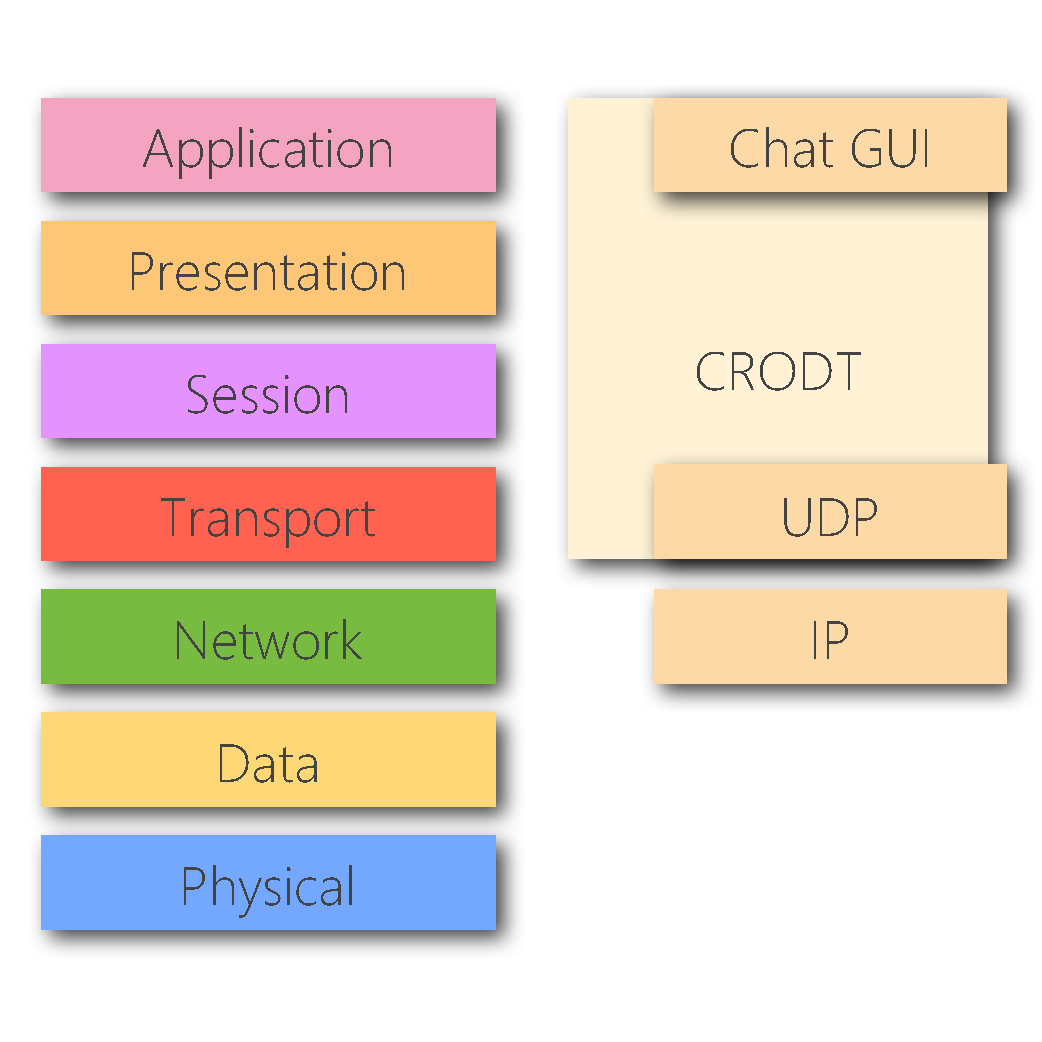
\includegraphics[scale=.38]{OSI.pdf}
\caption{{\"U}berblick des OSI-Schichtenmodells und der Zuordnung von CROP}
\label{fig:OSI}
\end{figure}
	\section{CROP}
		Das Content Relevance-Orientated Protocol (CROP) bezeichnet einen Protokollstack
der zur Relevanceabh{\"a}ngigen Daten{\"u}bertragung in Delay Tolerant Networks
eingesetzt wird.

	\section{Zeitmessung}
		Durch die unterschiedlichen Umlaufzeiten der Planeten um die Sonne wird eine
Umrechnung der Zeit auf der Erde zu der Zeit auf dem Mars ben{\"o}tigt.
Dadurch k{\"o}nnen die auf dem Mars aufgenommenen Daten zugeordnet werden.
F{\"u}r diese Berechnung wird das heliozentrische Weltbild (die Erde dreht sich
um die Sonne) genutzt.
Dabei bildet die Sonne den gemeinsamen Bezugspunkt f{\"u}r Erde und Mars.

Die Erde bewegt sich mit einer Geschwindigkeit von $27$ $\frac{km}{h}$ auf einer
elliptischen aber fast kreisf{\"o}rmigen Umlaufbahn um die Sonne (siehe Bild
\ref{fig:marsEarthOrbit}).

\begin{figure}[H]
	\centering
	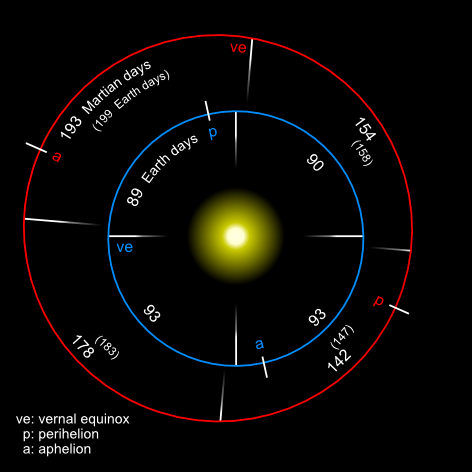
\includegraphics[scale=.5]{Mars_earth_orbit.png}
	\label{fig:marsEarthOrbit}
\end{figure}

Die Drehrichtung ist rechtl{\"a}ufig. Das hei{\ss}t die Bewegung erfolgt
entgegen dem Uhrzeigersinn um die Sonne. Mit gleichem Drehsinn erfolgt eine Eigenrotation
der Erde. Diese wird als sidierischer Tage bezeichnet und ist nach $23$ Stunden
und $56$ Minuten vollzogen. Die fehlenden $4$ Minuten, zu dem uns gel{\"a}ufigen
$24$ Stunden-Tag (Sonnentag), l{\"a}sst sich durch {\"a}u{\ss}ere Einwirkungen,
wie die Anziehungskraft der Sonne erkl{\"a}ren. Von dieser Betrachtung ausgehend, ben{\"o}tigt
die Erde f{\"u}r einen einmaligen Umlauf um die Sonne $365.2424$ Sonnentage, was
einem Erdenjahr (tropisches Jahr) oder einem terrianischen Jahr entspricht. 

Die selben Vorraussetzungen gelten ebenfalls f{\"u}r den Mars. Das Bild zeigt
\ref{fig:marsEarthOrbit} f{\"u}r den Mars eine viel elliptischere Bahn auf. Dies hat
eine Verschiebung der Tages und Jahreszeiten zur Folge. Somit ist auf dem Mars
ein Sonnentag exakt $24$ Stunden, $39$ Minuten und $35.24$ Sekunden lang und
wird "Sol" (Sol, engl. solar day) genannt. Nach $686.9710$ Erd-Sonnentagen bzw.
$669$ Sol hat der Mars die Sonne einmal vollst{\"a}ndig umkreist. Um eine Beziehung
und somit eine Umrechnung der Zeiten zwischen Planeten vorzunehmen, muss die
Einteilung der Monate und Jahreszeiten aus Sicht der Sonne, wie eingangs
erw{\"a}hnt, vorgenommen werden.

Im Weiteren soll eine M{\"o}glichkeit zur Umrechnung der Erdzeit auf Marszeit, nach
Robert Zubrin\todo{QUELLE},  welcher auch den Begriff "Sol" f{\"u}r einen
Marstag pr{\"a}gte, vorgestellt werden. Die nachfolgende Abbildung zeigt den von Zubrin entwickelten
Marskalender (Bild \ref{fig:marsEarthCalendar} links) im Vergleich zu dem uns
bekannten gregorianischen Kalender. Die Monate sind hierbei zur einheitlichen
Bestimmung in Form der lat. Namen der Tierkreiszeichen welche sie zu jener Zeit
von der Sonne aus gesehen durchziehen.

\begin{figure}[H]
	\centering
	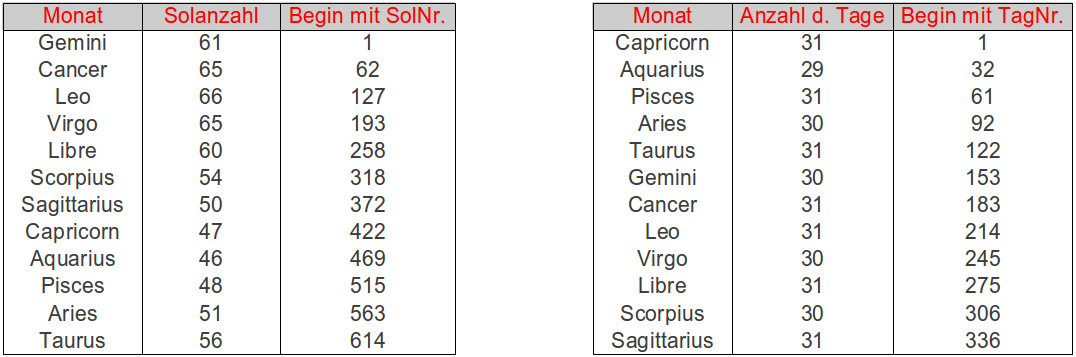
\includegraphics[width=\textwidth]{marsEarthCalendar.png}
	\label{fig:marsEarthCalendar}
\end{figure}

Bei der Umrechnung zwischen diesen beiden Kalendern, bezog sich Zubrin auf das
Jahr $1965$. Dort fielen der Beginn des Erdenjahres ($1.$ Januar), sowie der
Beginn des Marsjahres ($1.$ Gemini) aufeinander. Daraus ergab sich der
nachfolgende Ansatz:

\begin{equation}
	Marsjahr \quad = \quad (\frac{8}{15}) \quad * \quad (Erdjahr - 1961) \quad + \quad 1
	\label{eq:marsYear}
\end{equation}

Das Erdenjahr folgt einer dezimalen Darstellung und setzt sich wie in Formel
\ref{eq:earthYear} zusammen. Zum Tragen kommen hierbei das aktuelle Jahr, sowie
die numerischen Angaben von Tag ($numAktTag$) und Monat ($numAktMonat$) des zu
umrechnenden Datums. Dies wird ins Verh{\"a}ltnis zur Gesamtanzahl der Tage in einem
Jahr gesetzt.

\begin{equation}
	Erdjahr \quad = \quad aktuelleJahr + \frac{ (numAktMonat - 1) * 30.4 + (numAktTag - 1) }{365}
	\label{eq:earthYear}
\end{equation}

Diese soll am Beispiel der Marslandung der Sonde "Curiosity", am $6.$ August
$2012$, verdeutlicht werden.

Aus Gleichung \ref{eq:earthYear} wird zun{\"a}chst das dezimale Erdjahr berechnet.
Es ergibt sich:

\begin{eqnarray}
	Erdjahr \quad & = & \quad 2012 + \frac{ (8-1) * 30.4 + (6-1) }{365} \notag\\
	Erdjahr \quad & = & \quad 2012 + 0.59 \notag\\
	Erdjahr \quad & = & \quad 2012.59
\end{eqnarray}

In die Gleichung \ref{eq:marsYear} eingesetzt

\begin{eqnarray}
	Marsjahr \quad & = & \quad (\frac{8}{15}) * (2012.59 - 1961) + 1 \notag\\
	Marsjahr \quad & = & \quad 28.51
\end{eqnarray}

ergibt das Marsjahr $28$. Der jeweilige Tag und Monat des Jahres wird
schlussendlich durch die Gleichung \ref{eq:MarsMonthSol} und die Tabelle
\ref{fig:marsEarthCalendar} bestimmt.

\begin{eqnarray}
	Marstag \quad & = & \quad \#MarstageImJahr * restMarsjahr \\
	Marstag \quad & = & \quad 666 * 0.51 \notag\\
	Marstag \quad & = & \quad 340 Sol \notag
	\label{eq:MarsMonthSol}
\end{eqnarray}

Damit ist die Marssonde "Curiosity"' am $22.$ Sol im Sternbild Scorpius des 
Marsjahres $28$ auf dem Mars gelandet.

Zubrin's Ansatz weist einige Fehler auf, die auf den ersten Blick nichtig
erscheinen, aber auf weite Sicht starke Verschiebungen der Zeiten zur Folge
haben. Die Annahme, ein Erdenjahr sei immer $365$ Tage lang (siehe Formel
\ref{eq:earthYear}), kann nicht verallgemeinert werden. Vielmehr muss von einem
Mittel ausgegangen werden, da die L{\"a}nge eines Erdjahres aufgrund der sich
wechselnden Abst{\"a}nde zur Sonne variiert. Hier wird das sogenannte Tropische Jahr
herangezogen, welches $365.2424$ Tage lang ist. Davon ausgehend, ist eine
Korrektur des in der Formel \ref{eq:earthYear} angenommenen Verh{\"a}ltnisses von
Mars- zu Erdjahr (erster Term) auf $\frac{7.97}{15}$ notwendig (Nachweis ab
Formel \ref{eq:errorKorrektur}).

\begin{eqnarray}
	\frac{MarsJahr}{ErdJahr} \quad & = & \quad \frac{686.9710 \ Tage}{365.2424 \ Tage}
	\\
	\label{eq:errorKorrektur}  
	\frac{MarsJahr}{ErdJahr} \quad & = & \quad 1.88 \notag\\
	\notag\\
	x \quad & = & \quad \frac{15}{1.88} \notag\\
	x \quad & = & \quad 7.97 \notag
\end{eqnarray}

Damit w{\"u}rde sich das Landungsdatum der Marssonde auf den $16.$ Sol im Sternbild
Libre verschieben. Nach nur knapp $50$ Jahres der Zeitrechnung Mars stellt sich
schon eine Verschiebung von $66$ Sol ein. Dies zeigt dass eine exakte Umrechnung
der Daten von n{\"o}ten ist, um eine langfristige Aussage {\"u}ber das Datum und die
Zeit auf dem Mars zu machen.

\chapter{Stand der Technik}
  \label{cap:standDerTechnik}
Dieses Kapitel befasst sich mit dem aktuellen Stand der Technik. Dies
umfasst sowohl die gegenw{\"a}rtig eingesetzte Hardware, als auch bereits
entwickelte Protokolle zur interplanetaren Kommunikation.

\textbf{Mars Rover Curiosity} 

Der Mars Rover \textit{Curiosity} (Abbildung \ref{fig:Curiosity}) verf{\"u}gt
{\"u}ber einen RAD750 Prozessor von BAE-Systems.
Dieser hat eine Taktfrequenz von bis zu 200 MHz und kann 266 MIPS
verarbeiten. Desweiteren verf{\"u}gt \textit{Curiosity} {\"u}ber einen
Arbeitsspeicher von 256 MB und einen Flash-Speicher von 2 GB. Zus{\"a}tzlich hat
\textit{Curiosity} einen EPROM von 256 KB. Alle Bauteile sind dabei besonders
strahlungsresistent und unempfindlich gegen{\"u}ber gro{\ss}en
Temperaturschwankungen. Das genutzte Betriebssystem ist VxWorks (Ref.
\cite{WR}).
Zur Kommunikation nutzt der Rover einerseits das X-Band (7 - 8 GHz), welches zur
{\"U}bertragung von Statusdaten und zum Empfang von Steuerdaten genutzt wird.
Desweiteren verf{\"u}gt der Rover {\"u}ber ein Kommunikationssystem im UHF-Band
(0,4 GHz), welches f{\"u}r wissenschaftliche Daten mit hohem Datenvolumen
genutzt wird (bis zu 250 Mbit pro Tag, somit ca. 30 MB/Tag). Die Ausstattung an
wissenschaftlichen Instrumenten umfasst zehn Ger{\"a}te. Darunter z.B. zwei
Mastkameras welche je eine Aufl{\"o}sung von 1200 x 1200 Pixeln haben (1,44
Megapixel). Diese Kameras sind ebenfalls in der Lage 720p-Videos mit einer
Framerate von 10 Bildern pro Sekunde aufzunehmen. Hinzu kommen Spektrografen,
weitere Kameras, Sensoren etc., welche weitere Analysedaten beisteuern (Ref.
\cite{web5}).

\begin{figure}[H]
\centering
\includegraphics[scale=.12]{Curiosity.png}
\caption{Mars Rover Curiosity (Ref. \cite{imgCuriosity})}
\label{fig:Curiosity}
\end{figure}

\textbf{Deep Space Network}

Das Deep Space Network bezeichnet ein Netz von Parabolantennen, welche zur
Kommunikation mit Raumsonden, Satelliten sowie zu radio-
und radarastronomischen Zwecken dienen. F{\"u}r die NASA werden derzeit die
folgenden drei gro{\ss}en Stationen betrieben:

\begin{compactenum}[a)]
\item \textit{Goldstone Deep Space Communication Complex, Kalifornien, USA
(Abbildung} \ref{fig:Goldstone}\textit{)}
\item \textit{Madrid Deep Space Communication Complex, Madrid, Spanien}
\item \textit{Canberra Deep Space Communication Complex, Canberra, Australien}
\end{compactenum}

Das Deep Space Network wird auch f{\"u}r die Kommunikation zwischen dem Mars
Rover \textit{Curiosity} und der Erde genutzt. Die Anlagen liegen an exponierter Position
(zumeist h{\"u}geliges schalenf{\"o}rmiges Gel{\"a}nde). Dies soll den
Einfluss von St{\"o}rungen z.B. durch Radiofrequenzen reduzieren. Die Stationen
befinden sich je in einem Abstand von einem drittel Erd{\"a}quator um eine
fortw{\"a}hrende Kommunikation mit Raumfahrzeugen trotz Erdrotation zu
erm{\"o}glichen (Ref. \cite{web6}).

\begin{figure}[H]
\centering
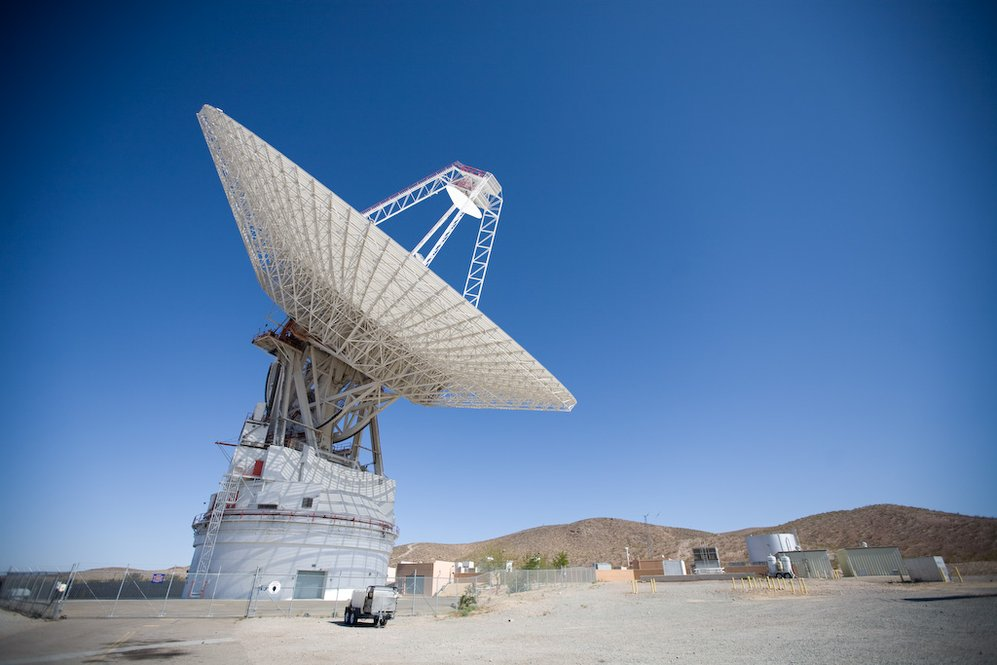
\includegraphics[scale=.3]{Goldstone.jpg}
\caption{Antenne der NASA Deep Space Network Einrichtung in Goldstone,
Kalifornien, USA (Ref. \cite{imgGoldstone})}
\label{fig:Goldstone}
\end{figure}

\textbf{Interplanitary Internet}

Das \gls{IPN} bezeichnet die Erweiterung des Internets
auf einen au{\ss}erirdischen Bereich. Die damit verbundenen {\"A}nderungen im
Vergleich zum irdischen Internet umfassen z.B. einen gesonderten Umgang mit
Latenzen, da diese beim \gls{IPN} im Minuten- bis Stundenbereich liegen. Die
Entwicklung von Protokollen f{\"u}r das \gls{IPN} obliegt dabei dem \gls{CCSDS}.

\textbf{Delay Tolerant Networking}

Das \gls{DTN} bezeichnet eine Protokollarchitektur f{\"u}r
Ende-zu-Ende Netzwerkverbindungen mit geringer Stabilit{\"a}t. Die Basis der
\gls{DTN} Netzwerkarchitektur stellt das von der NASA entwickelte \gls{IPN} dar. Ein wichtiger
Bestandteil dieser Netzwerke ist der Umgang mit gro{\ss}en Latenzen. Zudem
m{\"u}ssen die an der Kommunikation beteiligten Knoten (Teilnehmer)
Daten solange zwischenspeichern, bis der Empf{\"a}nger den Erhalt quittiert hat
(store-and-forward) (Ref. \cite{web3}).

\textbf{Bundle-Protokoll}

Die in den RFCs 4838 und 5050 festgelegten Anforderungen f{\"u}r \gls{DTN} sind
weitgehend unter der Bezeichnung Bundle-Protokoll bekannt. In diesem werden
Folgen von Datenbl{\"o}cken als B{\"u}ndel zusammengefasst. Jedes B{\"u}ndel enth{\"a}lt
dabei ausreichende semantische Informationen um eine etwaige Applikation
fortzusetzen. Exemplarisch sei hier ein Webbrowser angef{\"u}hrt, welcher ein
Bundle-Paket erh{\"a}lt und dadurch eine komplette Webseite anzeigt. Auch hier
erfolgt die {\"U}bertragung per \textit{store-and-forward}. Die eingesetzten
Transportprotokolle k{\"o}nnen dabei variieren (\gls{IP} basierend o.a.). Das
Bundle-Protokoll z{\"a}hlt zu den Overlay-Netzwerken, welche
auf einer bereits bestehenden Netzwerkstruktur aufsetzen (Ref. \cite{web1}).

\textbf{Licklider Transmission Protocol}

Das \gls{LTP} kann direkt auf dem Data Link Layer
aufsetzen oder aber auch unter \gls{UDP} laufen (siehe Abb. \ref{fig:LTP}). Das \gls{LTP}
wird zudem als Standard \textit{convergence layer protocol} (Zusammenfassung von
Transport- und Network-Layer) f{\"u}r das Bundle Protokoll genutzt. Das \gls{LTP}
wurde zur sicheren {\"U}bertragung von Daten zwischen einem Sender und einem
Empf{\"a}nger (Punkt-zu-Punkt) unter \gls{DTN} Bedingungen entwickelt. Das \gls{LTP}
entscheidet dabei zwischen wichtigen (red data) und unwichtigen Daten (green
data) und gew{\"a}hrleistet somit eine effiziente {\"U}bermittlung. Eine
{\"U}bertragung beginnt, sobald ein Link zwischen Sender und Empf{\"a}nger
besteht. Die zu sendenden Datenbl{\"o}cke werden beim \gls{LTP} in Segmente geteilt.
Handelt es sich um wichtige Daten werden w{\"a}hrend des Sendevorgangs
innerhalb der im \gls{LTP} verwendeten Segmente spezielle Flags gesetzt.
Diese einfach als Checkpoints bezeichneten Signale erfordern eine Quittierung
durch den Empf{\"a}nger, um so bei einem eventuellen Verbindungsabbruch ein
erneutes Senden des jeweiligen Datenpakets auszul{\"o}sen. Die Daten werden
solange beim Sender in einer \gls{FIFO} vorgehalten, bis der zugeh{\"o}rige
Checkpoint quittiert wurde. Wenn ein Checkpoint nicht quittiert wird, kann durch
einen ablaufenden Timer auf der Seite des Senders ein erneutes Senden
durchgeführt werden. Sowohl das Senden als auch Empfangen eines Blocks kann per
Signal abgebrochen werden. Zudem ist die Gr{\"o}{\ss}e der Segmente einstellbar um
diese an den jeweiligen Zweck anzupassen. Handelt es sich bei den zu sendenden
Daten um Daten mit geringerer Relevanz so ist keine
Best{\"a}tigung durch den Empf{\"a}nger notwendig.
Diese Daten werden direkt nach dem Versenden gel{\"o}scht (Ref. \cite{web4}).

\begin{figure}[H]
\centering
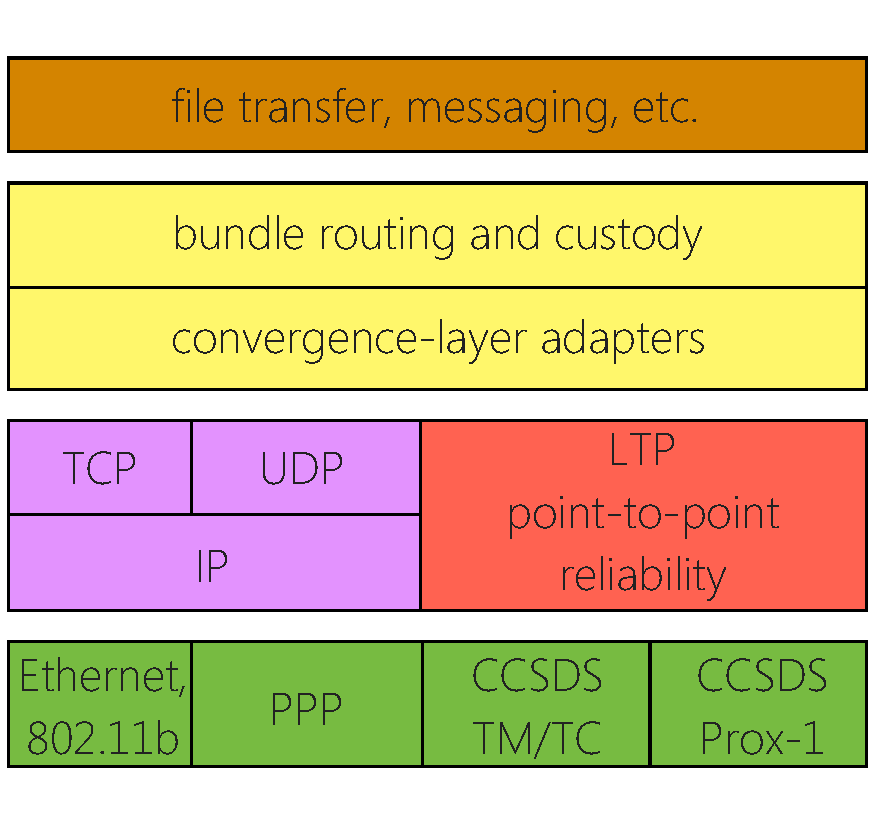
\includegraphics[scale=.4]{LTP.pdf}
\caption{Einordnung des LTP in das Kommunikationsmodell}
\label{fig:LTP}
\end{figure}

\textbf{Proximity-1}

Das \textit{Proximity-1 Space Link Protocol} ist das typischerweise genutzte
Data Link Layer/Physical Layer Protokoll in einem \gls{DTN} Stack. Damit komplettiert
dies zusammen mit dem Bundle Protokoll und dem \gls{LTP} die notwendigen
Protokollschichten eines \gls{DTN} Stack in einer interplanetaren Kommunikation.

\textbf{Stack einer interplanetaren Kommunikation}

Das \gls{DTN} Bundle Protokoll agiert als ein Overlay auf dem Transport Layer. Die
Abbildung \ref{fig:PSSBN} zeigt den Einsatz des Bundle Protokolls in einem
interplanetaren Kommunikationsansatz.
Dabei repr{\"a}sentiert der linke Teil des Stacks das Landefahrzeug auf der
Marsoberfl{\"a}che, welches das \gls{CFDP} {\"u}ber das Bundle Protokoll in
Verbindung mit dem \gls{LTP} nutzt.
Das Landefahrzeug wird schlie{\ss}lich {\"u}ber das Proximity-1 Space Link
Protokoll mit dem Orbiter (zweiter Stack von links) verbunden. Der dritte Stack
von links repr{\"a}sentiert z.B. eine \gls{DSN} Bodenstation. Der
Orbiter kommuniziert mit der \gls{DSN} Bodenstation {\"u}ber einen
\textit{deep-space-link} via Bundle Protokoll unter Nutzung des \gls{LTP}. Das
\gls{LTP} gew{\"a}hrleistet dabei eine verl{\"a}ssliche Verbindung. Der Stack auf der rechten {\"a}u{\ss}eren Seite
symbolisiert eine Missionskontrollstation, welche mit der \gls{DSN} Bodenstation
{\"u}ber einen klassische \gls{TCP}/\gls{IP} Stack kommuniziert. Das Bundle Protokoll
sichert dabei eine Ende-zu-Ende Kommunikation (Ref. \cite{DTNBundle}).

\begin{figure}[H]
\centering
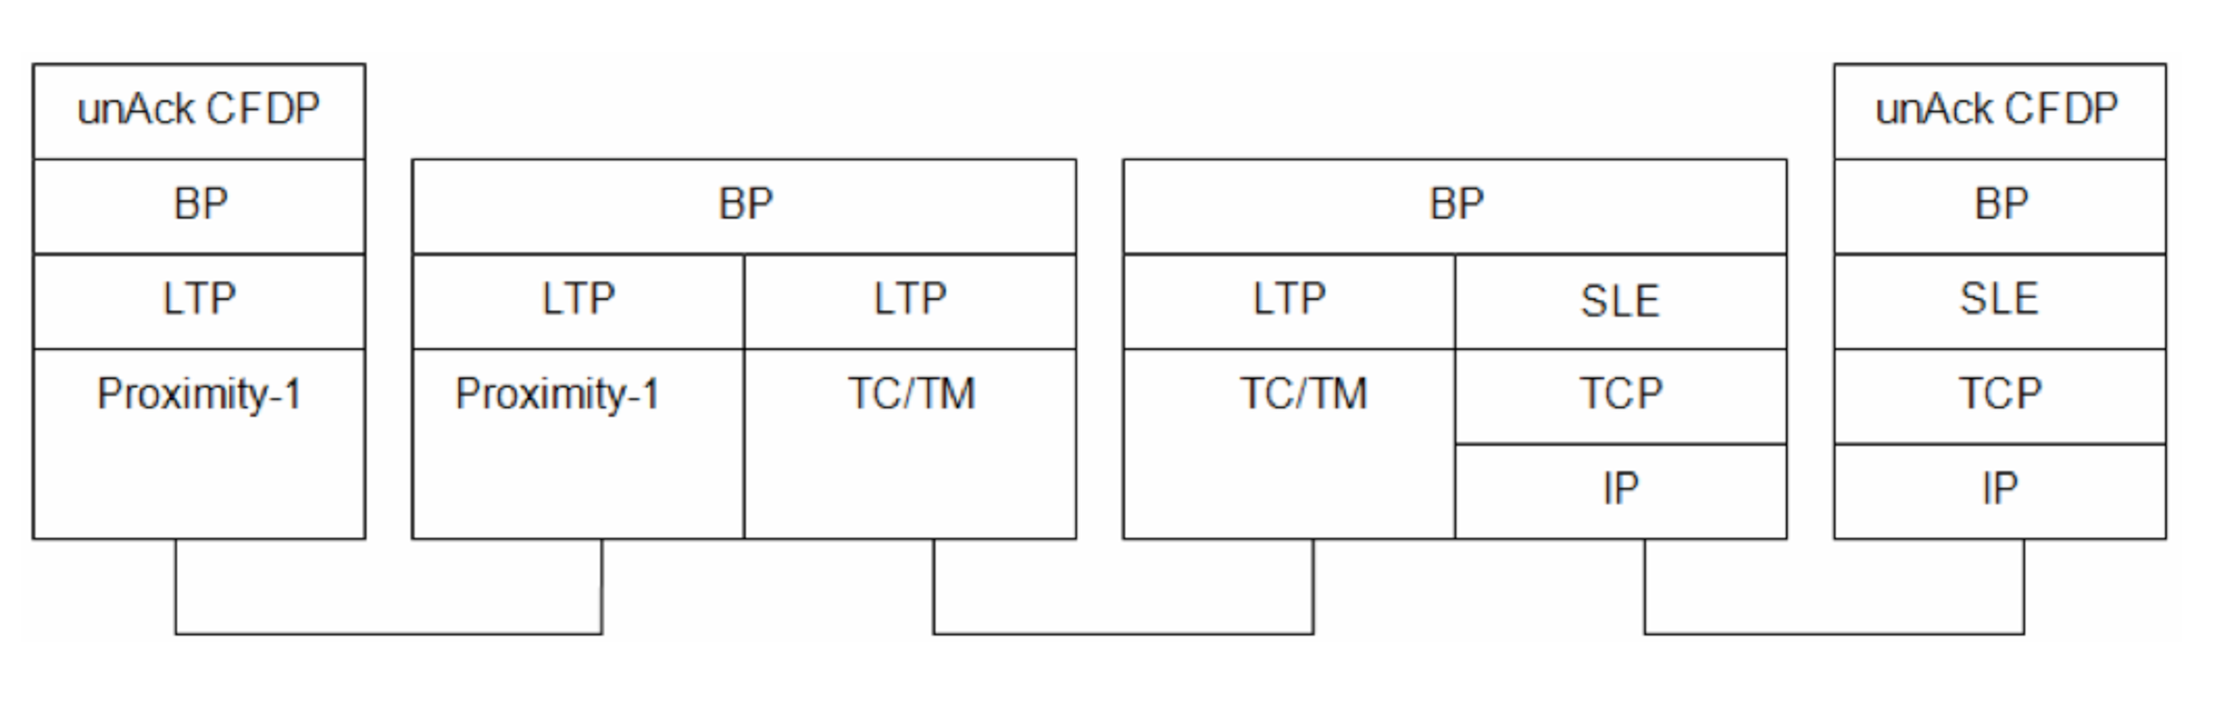
\includegraphics[scale=.35]{PSSBN.pdf}
\caption{Protokoll Stack eines interplanetaren Netzwerks (Ref.
\cite{DTNBundle})}
\label{fig:PSSBN}
\end{figure}

\textbf{\gls{QoS} vs. \gls{QoI}}

Die G{\"u}te eines Kommunikationsdienstes wird in irdischen Netzwerken
{\"u}blicherweise als Quality of Service (QoS) bezeichnet. Hierbei gibt es eine
Auswahl von Qualit{\"a}tsmerkmalen, mit Hilfe derer die Qualit{\"a}t eines
Service bewertet werden kann. Im Beispiel eines IP-Netzwerks w{\"a}ren dies
Parameter wie Jitter \footnote{zeitl. Schwankung (Taktzittern) in der
{\"U}bertragung von Digitalsignalen}, Latenzzeit, die Paketverlustrate sowie der Datendurchsatz.
Das QoS-Modell ist zwar theoretisch auch auf eine interplanetare Kommunikation
anwendbar (z.B. DTN/IPN), jedoch gleicht dieses aufgrund der hohen Latenzzeiten
in der {\"U}bertragung eher einer postalischen Kommunikation. Aus diesem Grund
wurde mit dem QoI (Quality of Interaction) ein speziell f{\"u}r diesen
Anwendungsfall konzipiertes Verfahren entwickelt (Ref. \cite{Daher2}). Dabei
werden, neben klassischen QoS-Merkmalen, welche ebenfalls genutzt werden
k{\"o}nnen, neue Verbindungsmerkmale betrachetet. Diese sind z.B. die
Dauer der Verbindung, {\"u}bertragene Daten pro Verbindung und andere Merkmale. 

\textbf{Ontologien}

Ontologien sind Sammlungen aus Inferenz- und Integrit{\"a}tsregeln um
Schlussfolgerungen auf komplexe Probleme zu beziehen. Ontologien werden zum
Austausch von Wissen in digitaler Form genutzt.

Bestandteile einer Ontologie:

 \begin{compactenum}[I]
     \item \textit{Begriffe}
     \item \textit{Typen}
     \item \textit{Instanzen}
     \item \textit{Relationen}
     \item \textit{Vererbung}
     \item \textit{Axiome}
   \end{compactenum}
\newpage   
\textbf{Vergleich der aktuellen Technologien mit CRODT}

Das CRODT-Framework stellt eine umfangreiche Sammlung an Funktionalit{\"a}ten
zur verf{\"u}gung. Diese {\"a}hneln in ihrem Einsatz zum Teil denen der
vorgestellten Protokolle (LTP/Bundle Protokoll). So unterscheidet das LTP
beispielsweise nach wichtigen und unwichtigen Daten (red/green data). Diese
Funktionalit{\"a}t gleicht in ihrer Intension der Relevanzevaluierung im
CRODT-Framework. Zudem sollen die Datenbl{\"o}cke aus den Messages, die durch
CROP verschickt werden, aufseiten des Empf{\"a}ngers direkt lesbar sein. Diese
Funktionalit{\"a}t gleicht der Bundle Strategie des Bundle Protokolls. Der
Einsatzgedanke der Ontologien innerhalb des CRODT-Frameworks hingegen
unterscheidet sich deutlich von den anderen angef{\"u}hrten Protokollen. Hierbei
sollen wichtige Daten automatisch erkannt und bewertet werden. Zudem ist das
Contentsplitting und die Relevanzevaluierung innerhalb von CRODT wesentlich
differenzierter (Werte zwischen 0 und 100). Die eigentliche {\"U}bertragung
erfolgt beim CRODT-Framework bisher Paketorientiert und ungesichert. Eine LTP
{\"a}hnliche Ende-zu-Ende Verbindung mit einer Empfangsquittierung w{\"a}re
jedoch auch denkbar. Zusammenfassend bietet das CRODT-Framework eine Sammlung an
Funktionalit{\"a}ten, welche im Vergleich zu den anderen Protokollen
differenzierter und umfangreicher ist. Der allgemine Grundgedanke ist jedoch
{\"a}hnlich.


\chapter{Konzept}
	\label{cap:konzept}

In diesem Kapitel werden vorrangig {\"U}berlegungen zur Fehlererkennung
und der Handhabung von Verbindungsabbr{\"u}chen bzw. fehlerhaften
{\"U}bertragungen dargelegt. In diesem Kontext werden die Notwendigkeiten einer
\gls{TTL} sowie die unterschiedlichen Optionen zur
Realisierung einer Datenkonsistenzpr{\"u}fung via CRC-Checksumme erl{\"a}utert.
Des Weiteren werden {\"U}berlegungen bez{\"u}glich der Entwicklung des
\gls{ROTP}-Stack aufgezeigt und analysiert. Dafür wird ein Protokoll
entwickelt, welches unterschiedliche Datenformate verpackt. Für die anstehende
Implementierung werden ausgehend von verschiedenen Anwendungsszenarien die
Schnittstellen der notwendigen Module bestimmt. Als Grundlage aller
{\"U}berlegungen diente das CRODT-Framework \cite{Daher}.

	\section{Vorüberlegung}
		\label{sec:Vorueberlegung}

\textbf{Ontologien}

Die bereits im Grundlagenkapitel erw{\"a}hnten Ontologien sind aufgrund ihrer
Komplexit{\"a}t und umfangreichen Einbindungszeit nicht Bestandteil des im
Verlaufe dieser Arbeit entwickelten Protokolls. Jedoch ist eine Einbindung
selbiger im weiteren Entwicklungsverlauf des Protokolls unabdingbar. Das
zuk{\"u}nftige Ziel ist es einerseits, mit Hilfe der Ontologien eine
automatisierte Priorisierung von Daten vorzunehmen, als auch eine manuelle
Priorisierungsm{\"o}glichkeit anzubieten (GUI). Somit kann ein auf dem Mars
befindliches System (z.B. ein Rover) selbstst{\"a}ndig entscheiden, welche
Informationen eine hohe Priorit{\"a}t zugewiesen bekommen. F{\"u}r einen
Einstieg in das Thema der Ontologieerstellung und deren Entwicklung im Bezug
auf die vorliegende Arbeit, sei auf die Paper von \cite{Noy2000} und \cite{Daher} verwiesen.

\textbf{Datenkompression}

Die Komprimierung von Daten gewinnt ein gro{\ss}es Ma{\ss} an Wichtigkeit, da
die zur Verf{\"u}gung stehende Bandbreite stark begrenzt ist. In Abh{\"a}ngigkeit der zu
verschickenden Daten (Bilder, Audio, Sensordaten etc.), sind hierbei
unterschiedliche Ans{\"a}tze denkbar. Einige dieser Ans{\"a}tze werden in
\cite{Kiely2006} und \cite{Kiely2007} vorgestellt. Im Rahmen der angefertigten
Arbeit wurde die Kompression allerdings nicht ber{\"u}cksichtigt.

\textbf{Time To Live}

Die \gls{TTL} bezeichnet die Lebensdauer eines Datenpakets und ist
dabei von unterschiedlichen Aspekten abh{\"a}ngig. So kann ein Paket einerseits nach
Ablauf eines Zeitraums oder nach einer bestimmten Anzahl
von Hops verworfen werden. Das Ablaufen durch den Hop\footnote{Ein Hop
bezeichnet eine Station einer Route auf dem Weg zum Ziel (Knoten)}-Zähler
ist dabei in einem Szenario der interplanetaren Kommunikation derzeit eher
unrealistisch, da zumeist eine Punkt-zu-Punkt Verbindung anvisiert wird (kein
intensives Routing {\"u}ber eine Vielzahl an Stationen). Somit w{\"a}re unter
Ber{\"u}cksichtigung einer interplanetaren Kommunikation eine
\gls{TTL}-Realisierung per Zeitstempel sinnvoller, da hier{\"u}ber, unter Ber{\"u}cksichtigung des
{\"U}bertragungskontextes, unrealistische {\"U}bertragungszeiten einfach erkannt
werden k{\"o}nnen.
Aufgrund der beschr{\"a}nkten Ressourcen unter interplanetaren
Kommunikationsumgebungen ist die Frage nach der Vorhaltedauer von
entscheidender Bedeutung. Damit wird die Speicherung der
Daten aufseiten des extraterrestrischen Senders bezeichnet. 
Eine m{\"o}gliche Entscheidungsgrundlage daf{\"u}r, wann Daten aus einer
\gls{FIFO} verworfen werden sollen, w{\"a}re die Wichtigkeit selbiger. So
k{\"o}nnen Daten geringer Relevanz direkt nach dem Senden gel{\"o}scht werden.
Wohingegen Daten hoher Relevanz erst nach Empfangsquittierung bzw. Ablauf des
\gls{TTL} Timers verworfen werden.

\textbf{Protokoll-Stack} \label{sec:Konzept_Protocolstack}

Die von der jeweiligen Anwendung an den \gls{CROP} Stack {\"u}bergebenen Daten
werden zun{\"a}chst in kleinere Datenbl{\"o}cke gesplittet. Diese Datenbl{\"o}cke
werden der Relevanz nach evaluiert und anschlie{\ss}end priorisiert.
Im Anschlu{\ss} daran werden die priorisierten Datenbl{\"o}cke der jeweiligen
Wertigkeit in einer \gls{FIFO} gespeichert. Danach werden im
Packetizer die Datenbl{\"o}cke h{\"o}chster Priorit{\"a}t zu einer
Nachricht zusammengefasst, die daraufhin an den \gls{UDP} Stack {\"u}bergeben
werden kann. Dieser grundlegende Ablauf ist in Abbildung \ref{fig:CRODT} schematisch
dargestellt.

\begin{figure}[H]
\centering
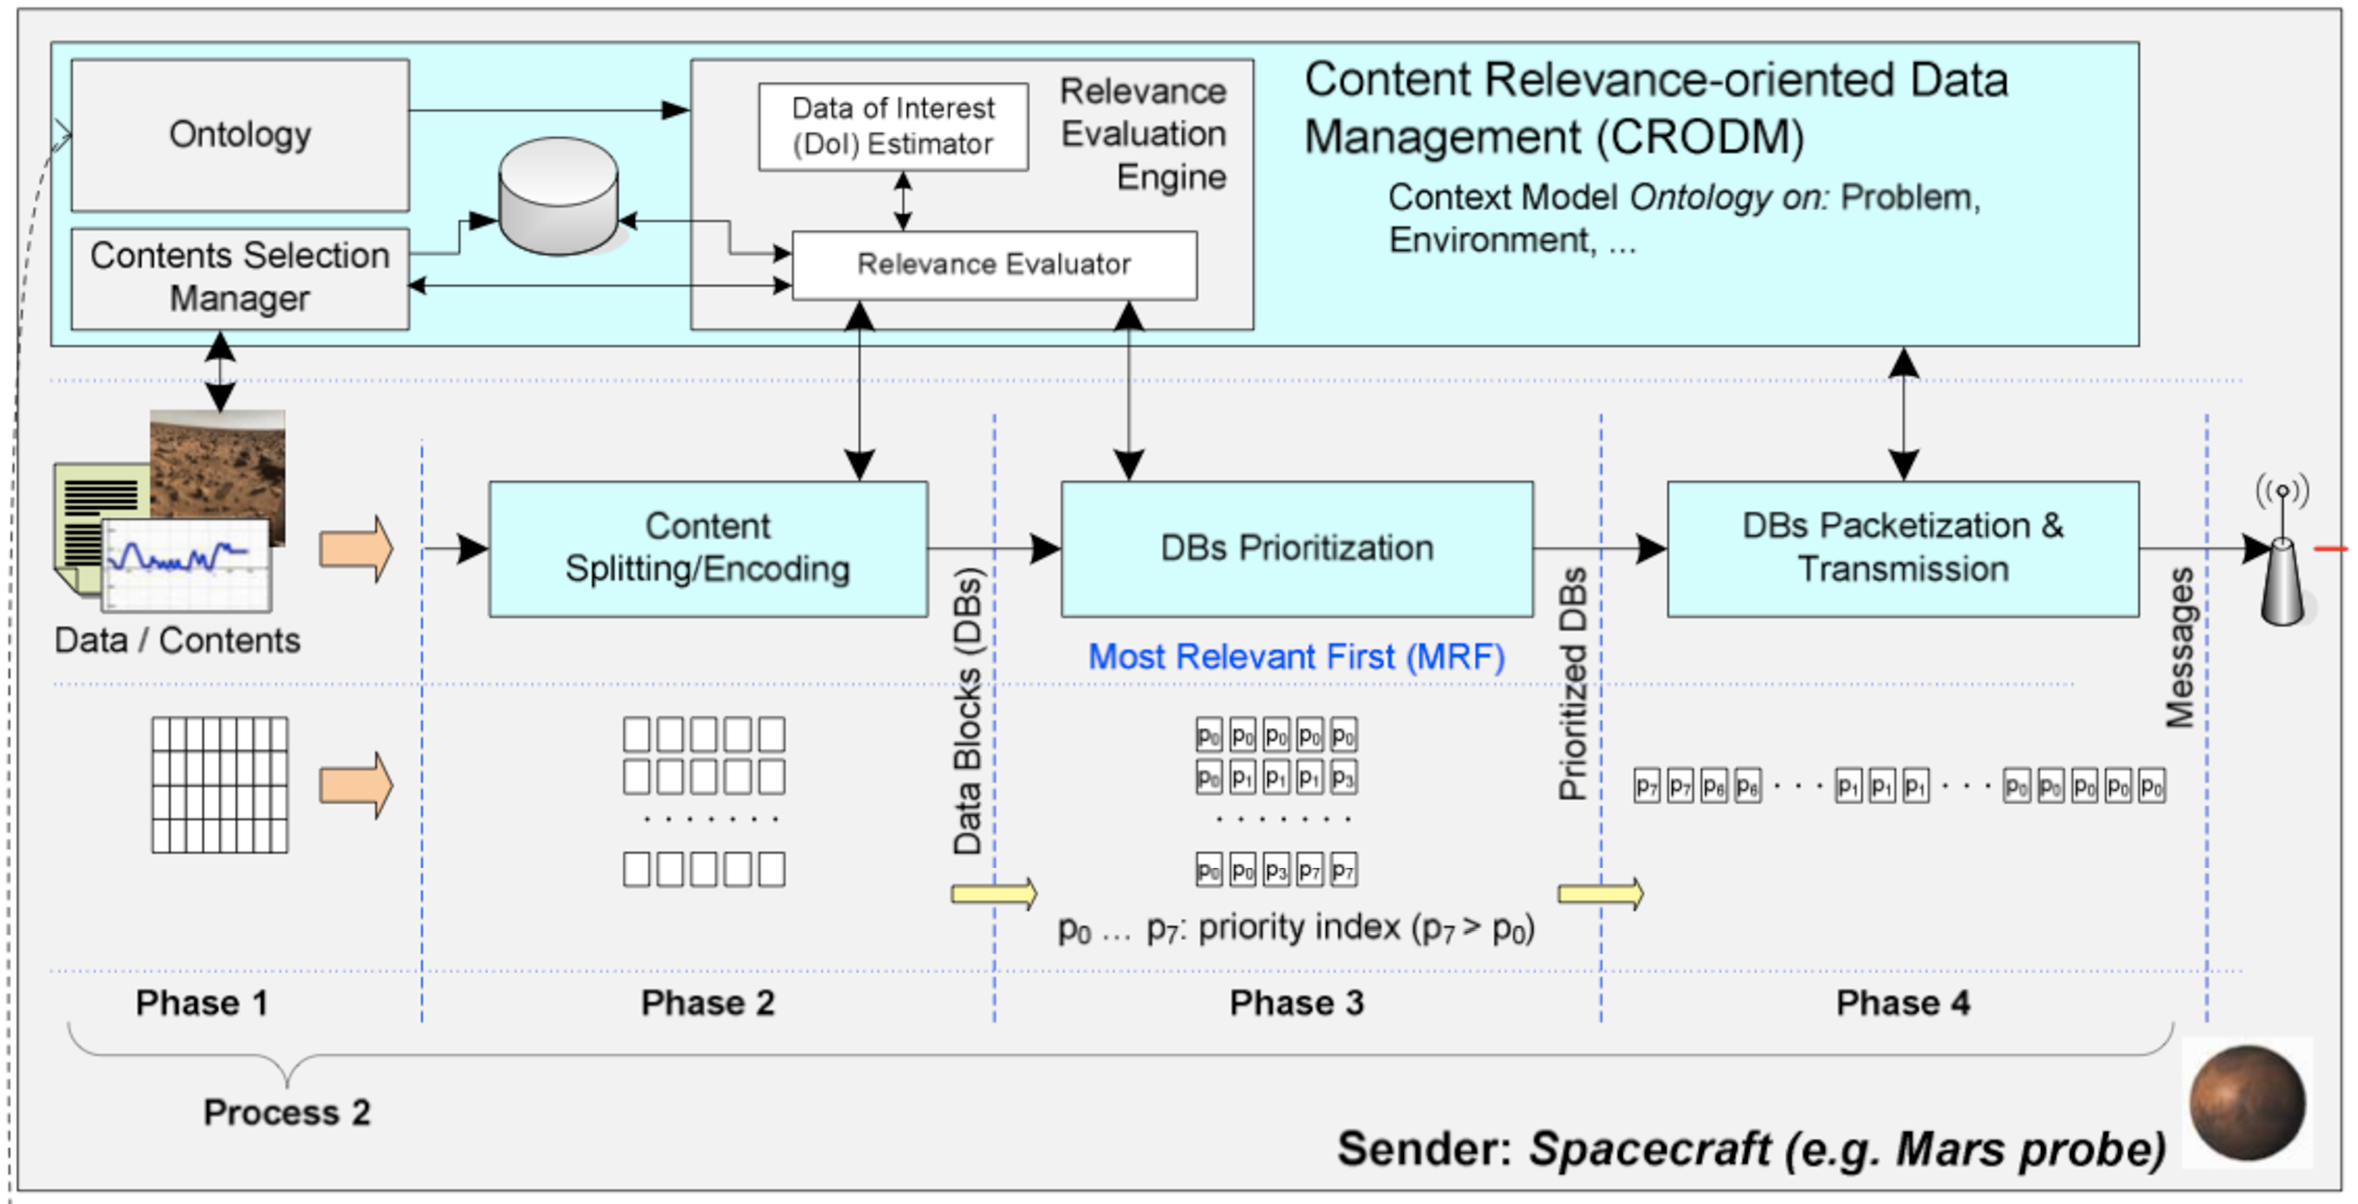
\includegraphics[scale=.3]{CRODT.pdf}
\caption[Das CRODT Framework]{Das CRODT Framework \cite{Daher}}
\label{fig:CRODT}
\end{figure}

In Abbildung \ref{fig:OSI_Stack} wird die Schachtelung der Daten
innerhalb des OSI-Stacks aufgezeigt. Dabei wird das Weiterreichen der Daten an
die jeweils n{\"a}chste Schicht des Stacks verdeutlicht. In jedem dieser Schritte wird dem neuen
Datenpaket der Header der aktuellen Schicht angeh{\"a}ngt und somit das
weitergereichte Datenpaket um notwendige {\"U}bersetzungsinformationen f{\"u}r
den Empf{\"a}nger erweitert. Auf der Empf{\"a}ngerseite erfolgt eine Invertierung dieses
Vorganges. 

\begin{figure}[H]
\centering
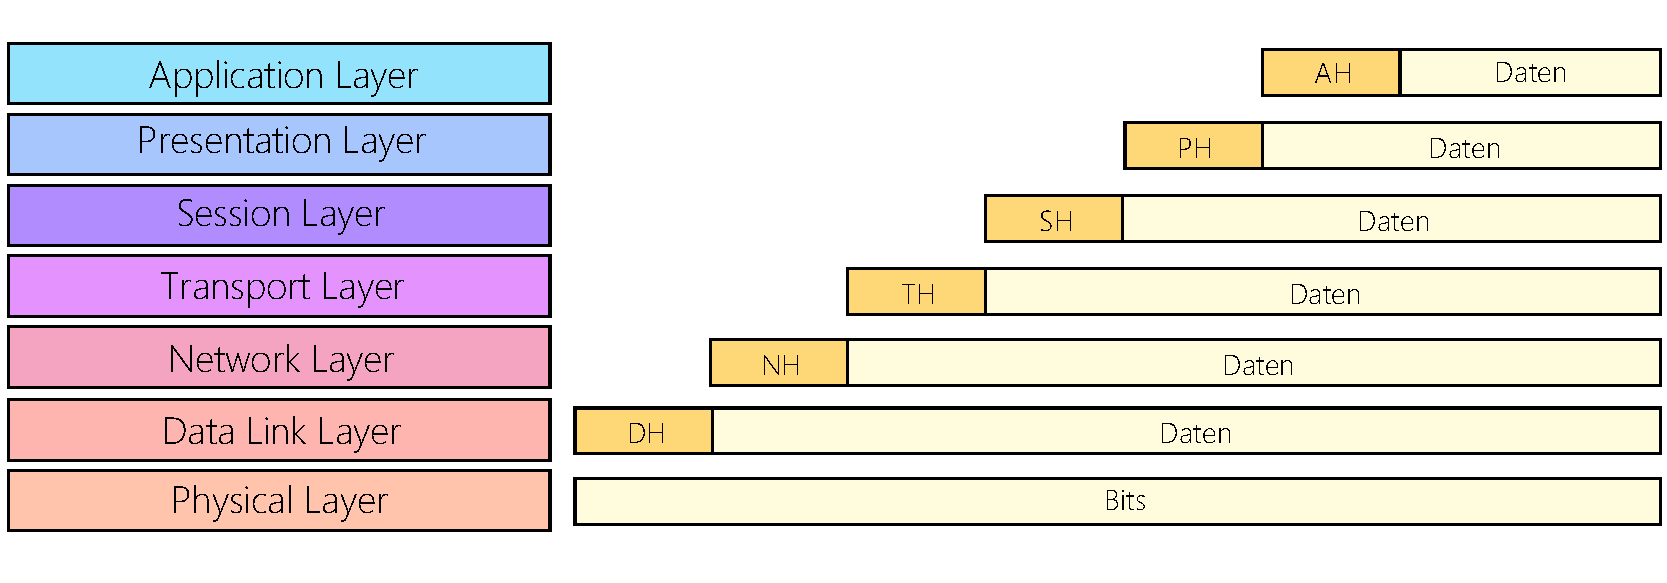
\includegraphics[scale=.5]{OSI_Stack.pdf}
\caption{Der OSI Stack}
\label{fig:OSI_Stack}
\end{figure}
 
Die Abbildung \ref{fig:CROP_Stack} zeigt die Handhabung im CROP-Stack
unter Nutzung des \gls{UDP}-Protokolls f{\"u}r die finale Daten{\"u}bertragung. Der
Application, Presentation und Session Layer des OSI-Modells
werden hierbei vereinfacht als Anwendungsschicht zusammengefasst.
Der Transport Layer des OSI-Modells entspricht der Transportschicht des
vereinfachten Modells. Die Internetschicht repr{\"a}sentiert den Network
Layer.
Der Data Link Layer und der Physical Layer des OSI-Modells werden zur
Netzzugangsschicht zusammengefasst. Dem OSI-Modell entsprechend wird eine
equivalente Darstellung der Paketerweiterung um den jeweiligen Header
hinzugef{\"u}gt. Der Protokollablauf sieht dabei nach Aufteilung der Daten in
Bl{\"o}cke und Zuweisung einer Priorit{\"a}t eine Zusammenfassung zu einer
Nachricht mit ausschließlich höher priorisierten Daten vor. Dieses Datenpaket
wird nun z.B. an den \gls{UDP}-Stack weitergegeben, anschlie{\ss}end um den
\gls{IP}-Header erweitert und dann entsprechend der
{\"U}bertragungsschnittstelle und deren Protokoll versandt. Die Nutzung von UDP
ist dabei beispielhaft zu betrachten, da andere Layer-4 Protokolle ebenso
infrage kommen.

\begin{figure}[H]
\centering
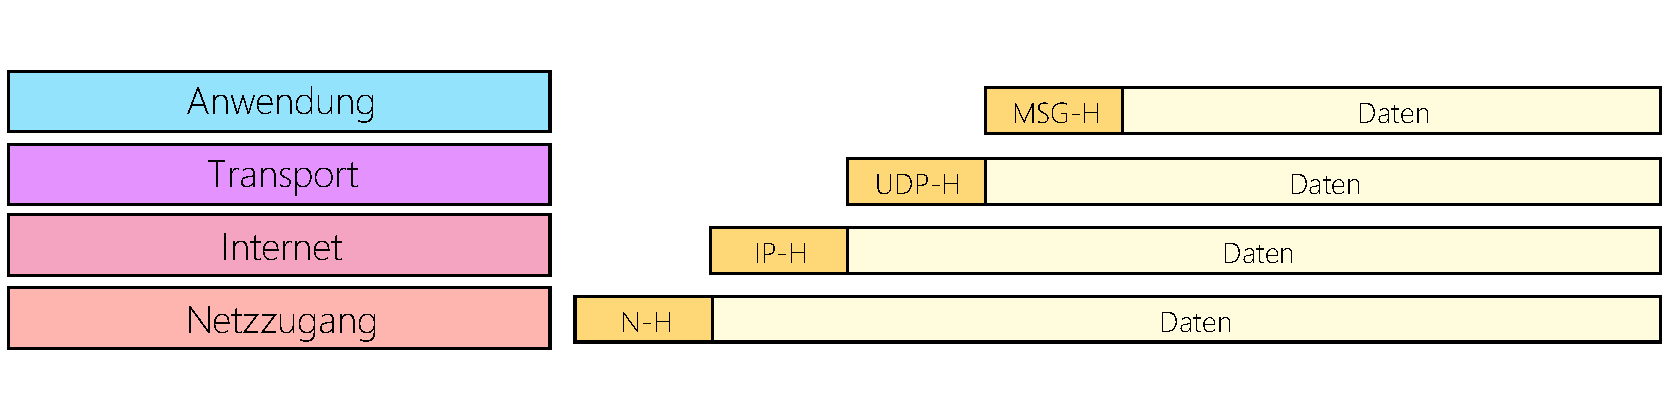
\includegraphics[scale=.5]{CROP_Stack.pdf}
\caption{Der CROP Stack}
\label{fig:CROP_Stack}
\end{figure}

\textbf{Error Correction Code}

Zur Fehlererkennung bzw. -korrektur wird ein CRC-Code verwendet. Dieser wird
innerhalb des Protokolls abhängig von der Paketgr{\"o}{\ss}e auf CRC 16 Bit oder
CRC 32 Bit eingestellt. Die Pr{\"u}fsumme wird durch einen mathematischen
Algorithmus ermittelt und dann mit dem Paket {\"u}bertragen. Wenn der
Empf{\"a}nger die R{\"u}ckrechnung unter Einbeziehnung der Pr{\"u}fsumme
vornimmt, kann anhand des Ergebnisses ermittelt werden, ob das Paket
verf{\"a}lscht wurde. Die Berechnung einer Checksumme funktioniert dabei wie
folgt:

Das zu {\"u}bertragende Datenframe sei exemplarisch gegeben als: 11 0101 1011.
Des Weiteren wird ein CRC-Generatorpolynom ben{\"o}tigt, welches im Beispiel als
$G(x) = x^4 + x + 1$ gegeben sei. Die daraus resultierende Schreibweise in Generatorbits lautet: 10011
($1*x^4+0*x^3+0*x^2+1*x^1+1*x^0$).
Anschließend wird eine erweiterte Darstellung des zu {\"u}bertragenden Frames
erzeugt, woraus der folgende Ausdruck hervorgeht: 11 0101 1011 0000
(Frame-0-Bits; Erweiterung des Datenframes um die Ordnung des Generatorpolynoms
in Nullen). Danach erfolgt eine Division des erweiterten Frames durch das
Generatorpolynom, welche nachfolgend dargestellt ist.

\makeatletter
\def\cline#1{\noalign{\vskip-2ex}\@cline#1\@nil}
\makeatother

\begin{figure}[H]
\jot-0.6mm
\begin{alignat*}{14}
1&1&0&1&0&1&1&0&1&1&0&0&0&0& : 10011=1100001010 \\
1&0&0&1&1\\ \cline{1-5}
&1&0&0&1&1& \\ 
&1&0&0&1&1& \\ \cline{2-6}
&&0&0&0&0&1& \\ 
&&1&0&0&1&1& \\ \cline{3-7}
&&&0&0&0&1&0& \\                                                 
&&&1&0&0&1&1& \\ \cline{4-8}
&&&&0&0&1&0&1& \\                                               
&&&&1&0&0&1&1& \\ \cline{5-9}
&&&&&0&1&0&1&1& \\                                           
&&&&&1&0&0&1&1&  \\ \cline{6-10}                                                                                  
&&&&&&1&0&1&1&0& \\                                           
&&&&&&1&0&0&1&1& \\   \cline{7-11}                                                                                      
&&&&&&&0&1&0&1&0& \\                                         
&&&&&&&1&0&0&1&1& \\ \cline{8-12}                                                                                     
&&&&&&&&1&0&1&0&0& \\                                       
&&&&&&&&1&0&0&1&1& \\ \cline{9-13}                                                                               
&&&&&&&&&0&1&1&1&0& \\                                     
&&&&&&&&&1&0&0&1&1& \\ \cline{10-14}    
&&&&&&&&&&1&1&1&0& 
\end{alignat*}
\caption{Modulo-2-Division} 
\end{figure}

Der Rest $1110$ dieser Modulo-$2$-Division wird an das
urspr{\"u}nglich zu {\"u}bertragende Frame $11 0101 1011$ angeh{\"a}ngt. Somit
ergibt sich das Frame inklusive Pr{\"u}fsumme: $11 0101 1011 1110$. Der
Empf{\"a}nger kann damit {\"u}berpr{\"u}fen, ob das Frame korrekt {\"u}bertragen
wurde. Dazu wird dieses durch das Generatorpolynom (Generatorbits) geteilt.
Das Ergebnis muss dabei null sein. Das im Beispiel genutzte Polynom kann mit der
Ordnung $4$ ($2^4=16$) auf Daten von $16$ Bit Länge angewendet werden. Das
Polynom $x16+x12+x5+1$ wird hingegen beispielsweise beim CRC-CCITT $16$ Bit-Verfahren
genutzt und kann auf Datenframes bis zu einer Gr{\"o}{\ss}e von $2^{16}=65536$
Bit angewendet werden \cite{web2}.


	\newpage
	\section{Protokoll-Design}
		\label{sec:ProtokolDesign}

\textbf{Message Header}

Eine zentrale Rolle bei der Entwicklung des Aufbaus und der Strukturierung
spielte der Nachrichtenheader.
Dieser beinhaltet Informationen, die zum eindeutigen Versenden und Identifizieren der
mitgelieferten Daten notwendig sind. Dazu gehören die Versionsnummer,
die Konfiguration, die Länge der Nachricht und die genauen Adressen
des Senders und Empfängers. Neben dem Header sind die verpackten Daten, der
sogenannte Payload, und ein CRC-Code zur Fehlerüberprüfung der Nachricht
vorhanden. In Abbildung \ref{fig:DatenaufschluesselungMessage} ist der Header
einer Nachricht im Detail dargestellt.

\begin{figure}[H]
	\centering
	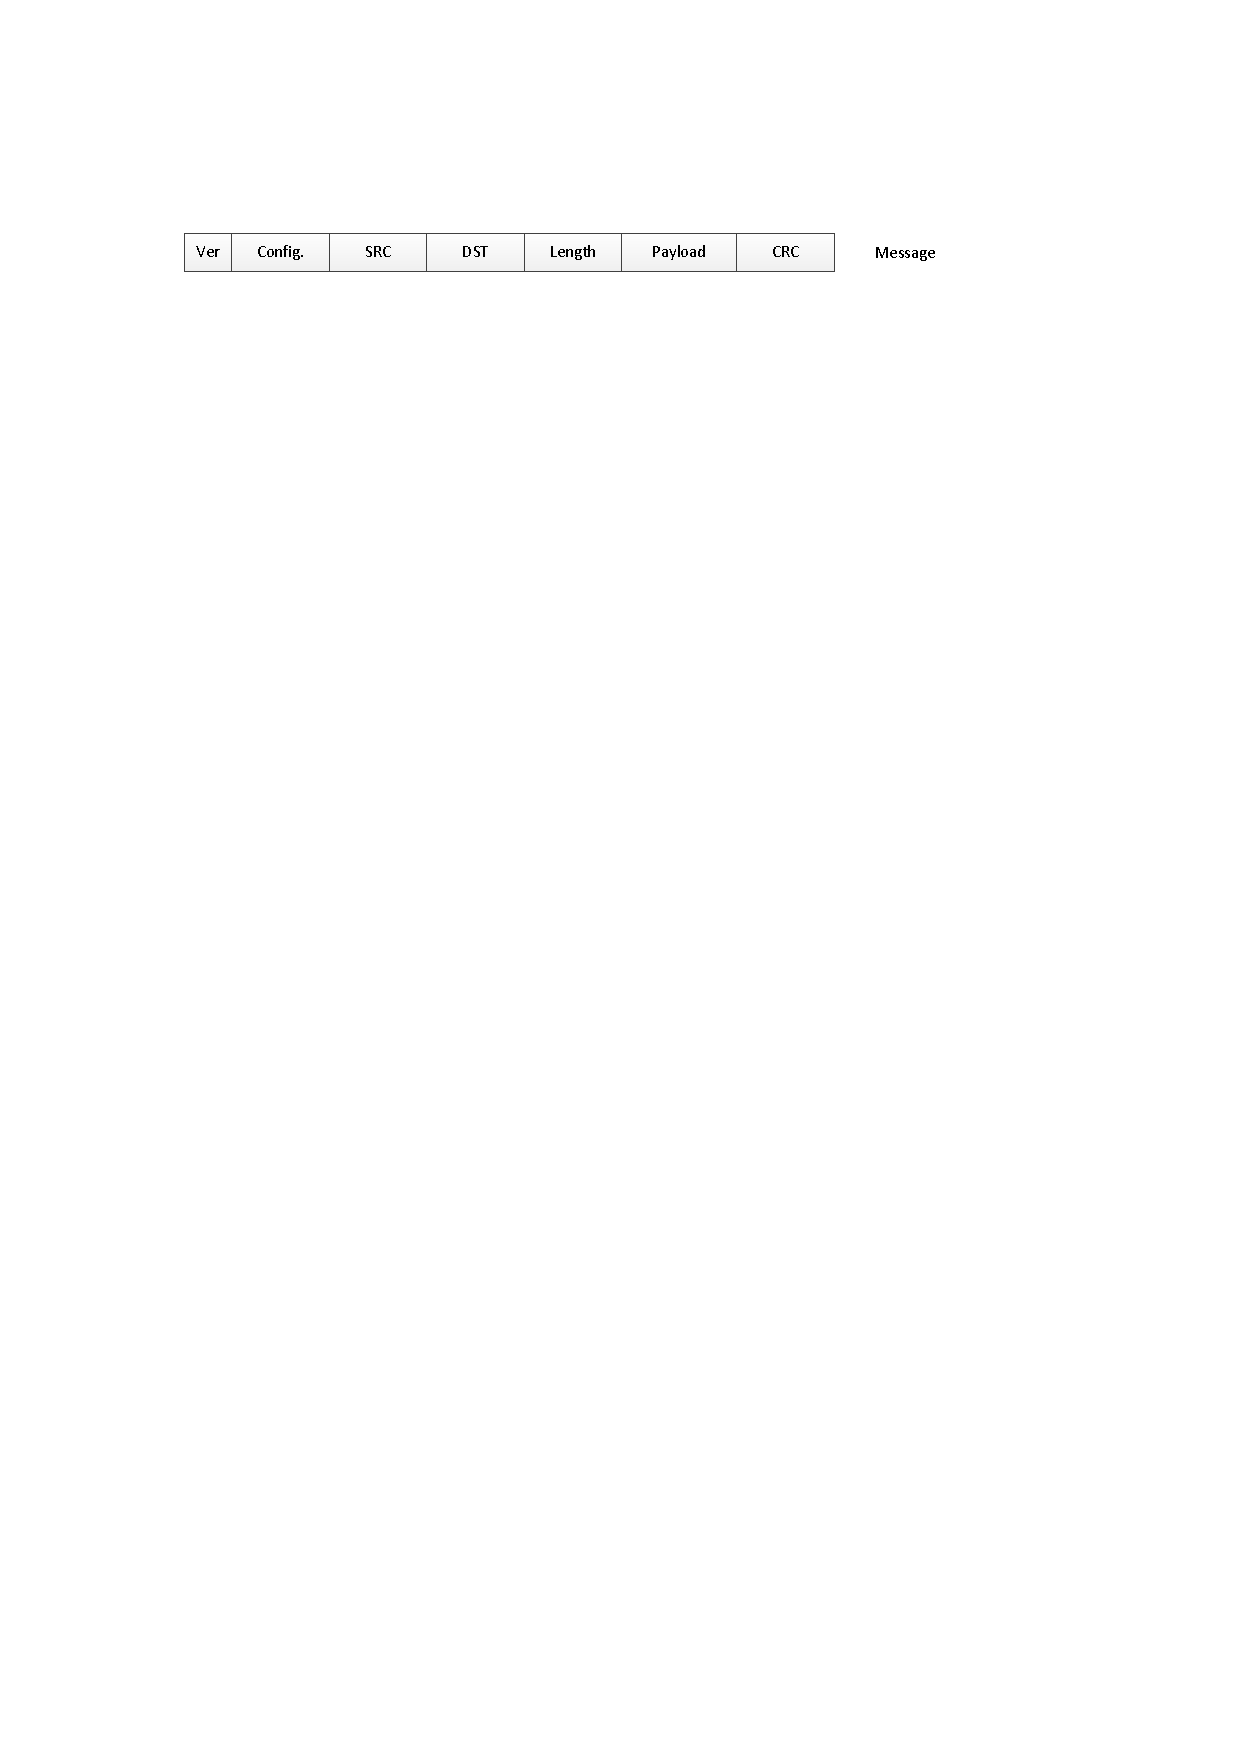
\includegraphics[width=\textwidth]{DatenaufschluesselungMessage.pdf}
	\caption{Datenaufschlüsselung der Nachricht}
	\label{fig:DatenaufschluesselungMessage}
\end{figure}

Die Versionsnummer belegt die ersten vier Bits des Headers. Diese
signalisiert dem Empfänger mit welcher Version des Protokolls die Nachricht
verpackt und versandt wurde. Danach folgt die Konfiguration. Mit Hilfe dieser,
können Einstellungen vorgenommen werden, welche die Größe der gesamten Nachricht
beeinflussen. Somit ist in speziellen Fällen eine bandbreitenschonende
Übertragung der Nachricht möglich, da keine ungenutzten Informationen oder Bits
vorhanden sind. Für die Konfiguration wurden $12$ Bits reserviert. Die ersten drei Bits
bestimmen das Adressformat. Dieses ermöglicht das Aufsetzen des Protokolls auf
bereits bestehenden Standards, wie IPv6 oder das Bundle-Protokoll.
Die verbleibenden neun Bits sind für zusätzliche Einstellungsmöglichkeiten zur Erweiterung des
Protokolls reserviert. Die Bitvergabe der Adressen von Sender und Empfänger
erfolgt dynamisch und in Abhängigkeit von der Konfiguration.
Dies ist für die Nutzung unterschiedlicher Übertragungsprotkolle notwendig.
Für IPv6 werden $256$ Bit bereitgestellt. Dies sind jeweils $128$ Bit für
die Sender- und Empfängeradresse. Die Länge repräsentiert die Größe der gesamten
Nachricht in Bytes und belegt die nächsten $24$ Bits.
Der vorletzte Bestandteil der Nachricht, der sogenannte Payload, beinhaltet die
eigentlichen Daten und besteht aus mehreren Datenblöcken. Zusätzlich werden am
Ende die Prüfsummenbits zur Fehlererkennung hinzugefügt. Diese sind $16$ Bits lang,
wenn die Gesamtlänge der Nachricht kleiner gleich $2^{16}$ Bytes ist.
Andernfalls beträgt die Länge $32$ Bits. Durch diese Unterteilung kann
Overhead vermieden werden wobei eine {\"U}bertragung gr{\"o}{\ss}erer
Nachrichten dennoch gew{\"a}rleistet bleibt.

\begin{figure}[H]
	\centering
	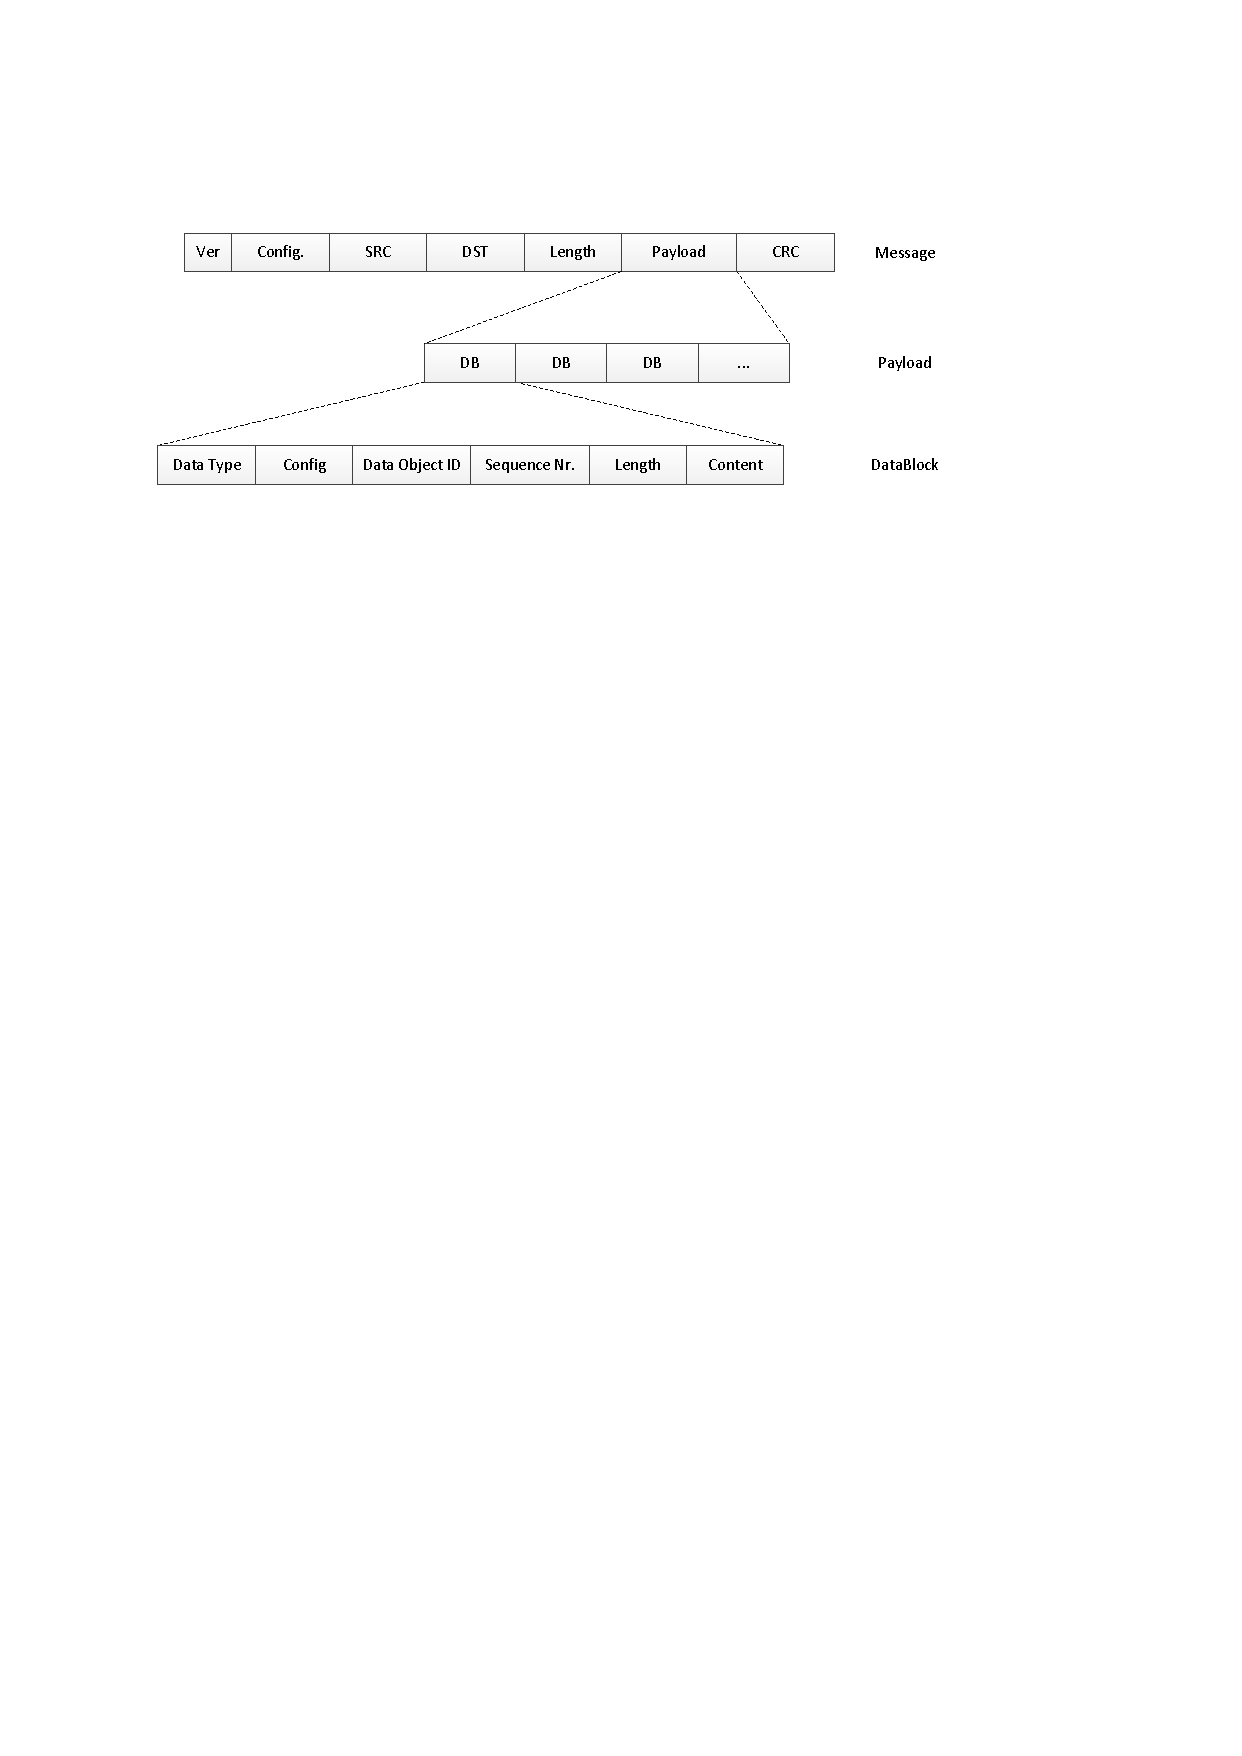
\includegraphics[width=\textwidth]{DatenaufschluesselungDB.pdf}
	\caption{Aufschlüsselung der Datenblöcke}
  \label{fig:DatenaufschluesselungDB}
\end{figure}

\textbf{Datenblockheader}

Eine schnelle und eindeutige Zuordnung eines einzelnen Datenblocks auf der
Empfängerseite, stand bei der Entwicklung des Headers im Mittelpunkt.
Dies bedeutet, dass neben der Bitvergabe eine genaue Überlegung über die
richtige Reihenfolge notwendig ist. Hierzu gibt es drei Ansätze, welche in
Abbildung \ref{fig:DatenblockVarianten} dargestellt sind.

\begin{figure}[H]
	\centering
	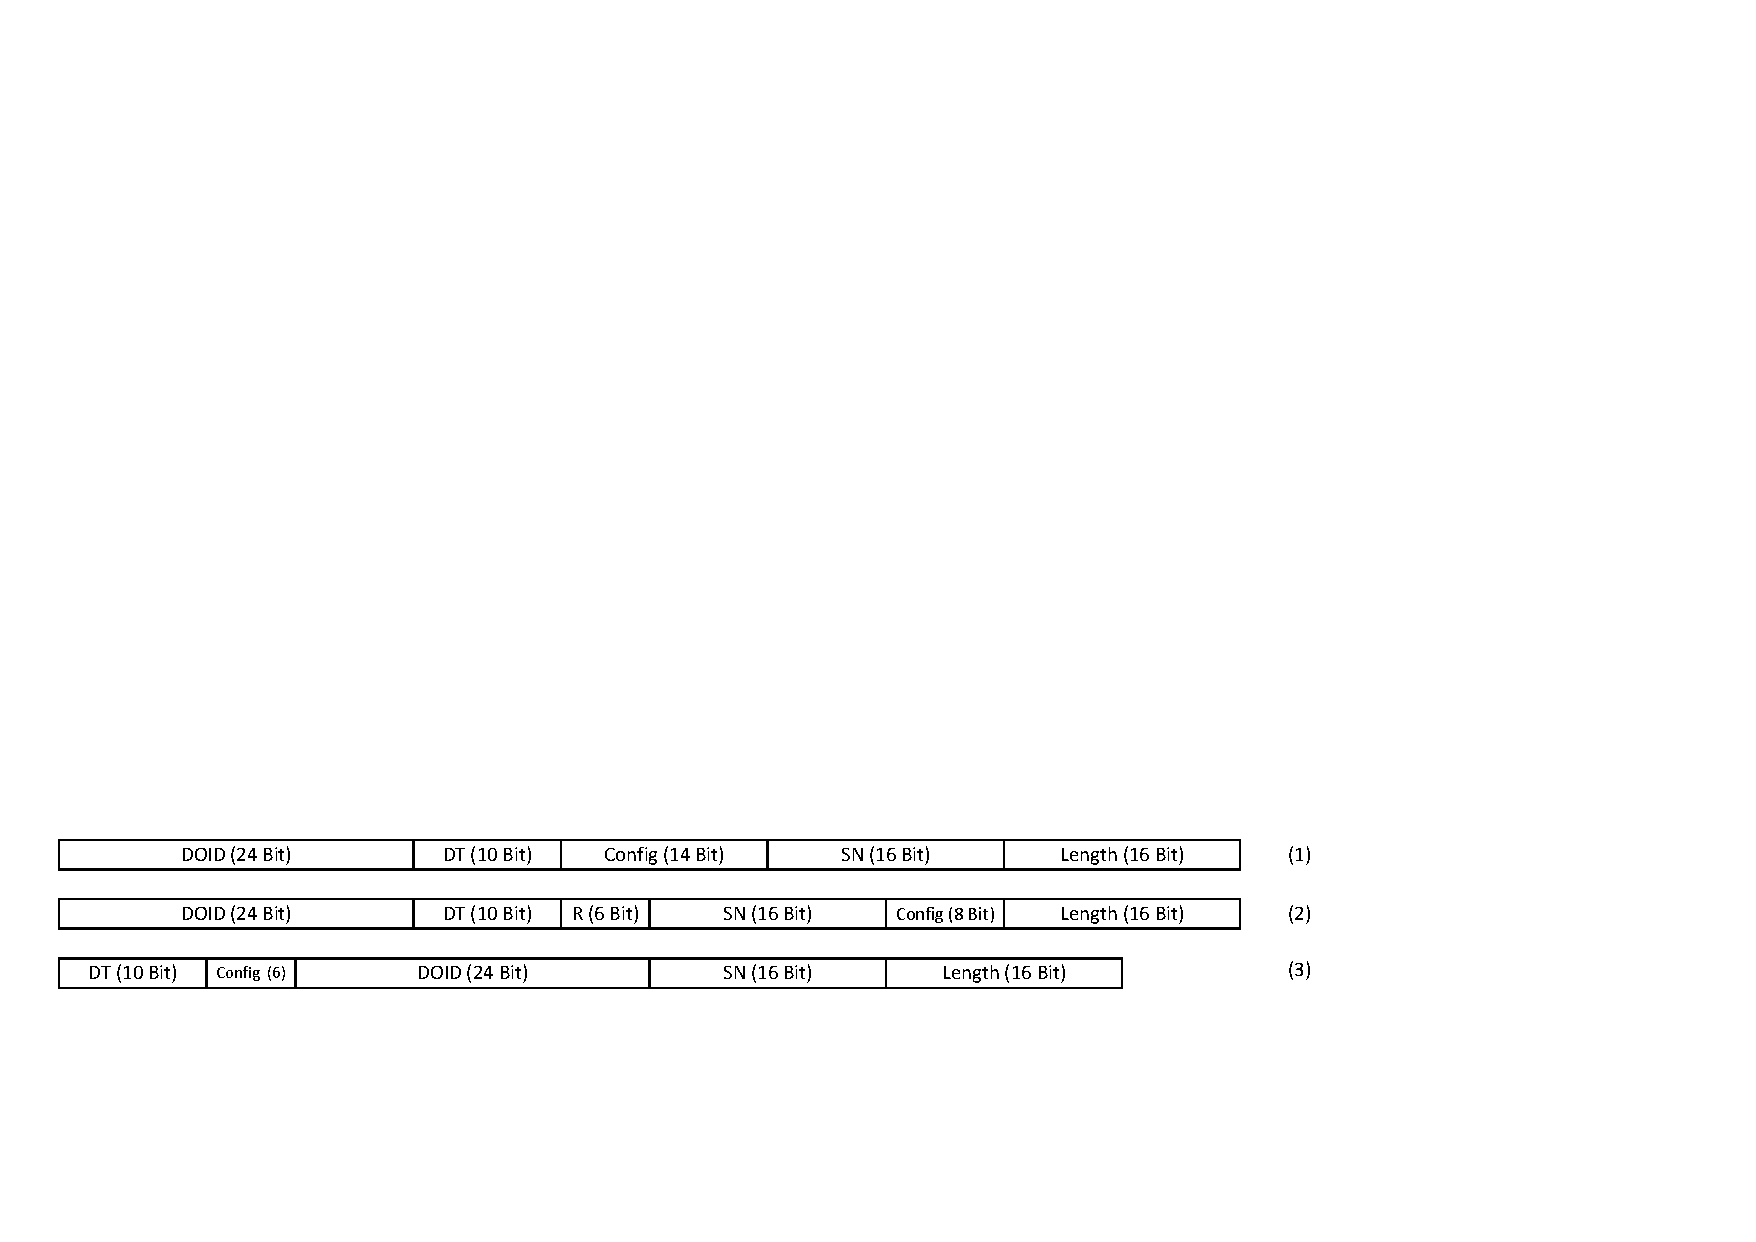
\includegraphics[width=\textwidth]{DatenblockVarianten.pdf}
	\caption{Ansätze des Datenblockheaders}
  \label{fig:DatenblockVarianten}
\end{figure}

Ein Datenblock besteht aus den folgenden Teilen: \gls{DOID}, Datentyp,
Konfiguration, Sequenznummer und der Länge des Datenblocks. Die \gls{DOID}
repräsentiert die Datei (Bild, Text, Sensorwerte,\etc) dem der Datenblock
angehört. Das Differenzieren der einzelnen Datenblöcke untereinander erfolgt
mittels der Sequenznummer. Durch die Einführung eines Datentyps im Header wird
der Bereich der \gls{DOID} indirekt vergrößert. Dies ist aufgrund der
eindeutigen Zuordnung einer \gls{DOID} zu einem Datentyp möglich.
\newline
Ausgegangen wurde anfangs von je acht Bit für den Datentyp und
die Konfiguration.
In diesem Zusammenhang wurde hinterfragt, ob die Bitvergabe ausreicht,
da sehr viele verschiedene Datentypen und Formate existieren. Infolgedessen
wurde, wie in Variante $1$ zu sehen, ein zusätzliches Byte zur Verfügung
gestellt. Dieses ist aufgeteilt in zwei Bit für den Datentyp und sechs Bit für
die Konfiguration. Die Idee hinter dieser Variante war, dass der Datenblock als
erstes über die \gls{DOID} und im Folgenden dem zugeordneten Datentyp identifiziert
wird. Anschließend sollten die Konfiguration und die Sequenznummer folgen.
Ein ähnlicher Aufbau gilt ebenfalls für Möglichkeit $2$, bei der die restlichen
sechs Bit zur Vorreservierung größerer Datentypen genutzt wurden. Dies war
bezüglich des Datentyps und der Menge unterschiedlicher Datenblöcke die bessere
Variante. Eine effektivere Maßnahme ergab sich am Ende nicht aus dem
Spendieren eines zusätzlichen Bytes, sondern aus einer anderen Reihenfolge in
der die Bestandteile im Header angeordnet sind. Wie in Variante $3$ ersichtlich,
wurden sechs Bit gespart. Dadurch wird zuerst jeder Datenblock anhand
seines Datentypes identifiziert und anschliessend durch die \gls{DOID} und die
Sequenznummer spezifiziert. Danach folgt die Konfiguration mit $6$ Bits.
Dabei sind die vordersten drei Bits die Kompression des Datenblockheaders, damit
kann die Länge der \gls{DOID}, der Sequenznummer und die Länge des gesamten
Datenblockes varrieren. Dadurch können auch kompakte Blöcke effizient
verschickt werden.
Das vierte Bit gibt an, ob ein Zeitstempel nach dem Header und vor einem
Datenpaket mit einer Länge von $8$ Byte gesetzt wird.
Dieses Bit wurde in der Konfiguration eingeführt, weil bei einigen Datentypen
nicht zwingend eine Zeitangabe benötigt wird und somit Overhead vermieden
werden kann. Für Daten mit konstanter aber geringer Größe können mehrere Werte
gleichzeitig in einem Datenblock platziert werden. Diese besitzen bei
gesetztem Zeitbit eine eigene Zeitangabe. Die Abbildung
\ref{fig:uebersichtdatenaufschluesselung} stellt diese Sachverhalte noch einmal
übersichtlich dar, diese werden im Anhang \ref{sec:messtabellen} noch
einmal in einer geb{\"u}hrenden Ausführung dargestellt.

\begin{figure}[H]
  \centering
  \subfigure[Sensor]{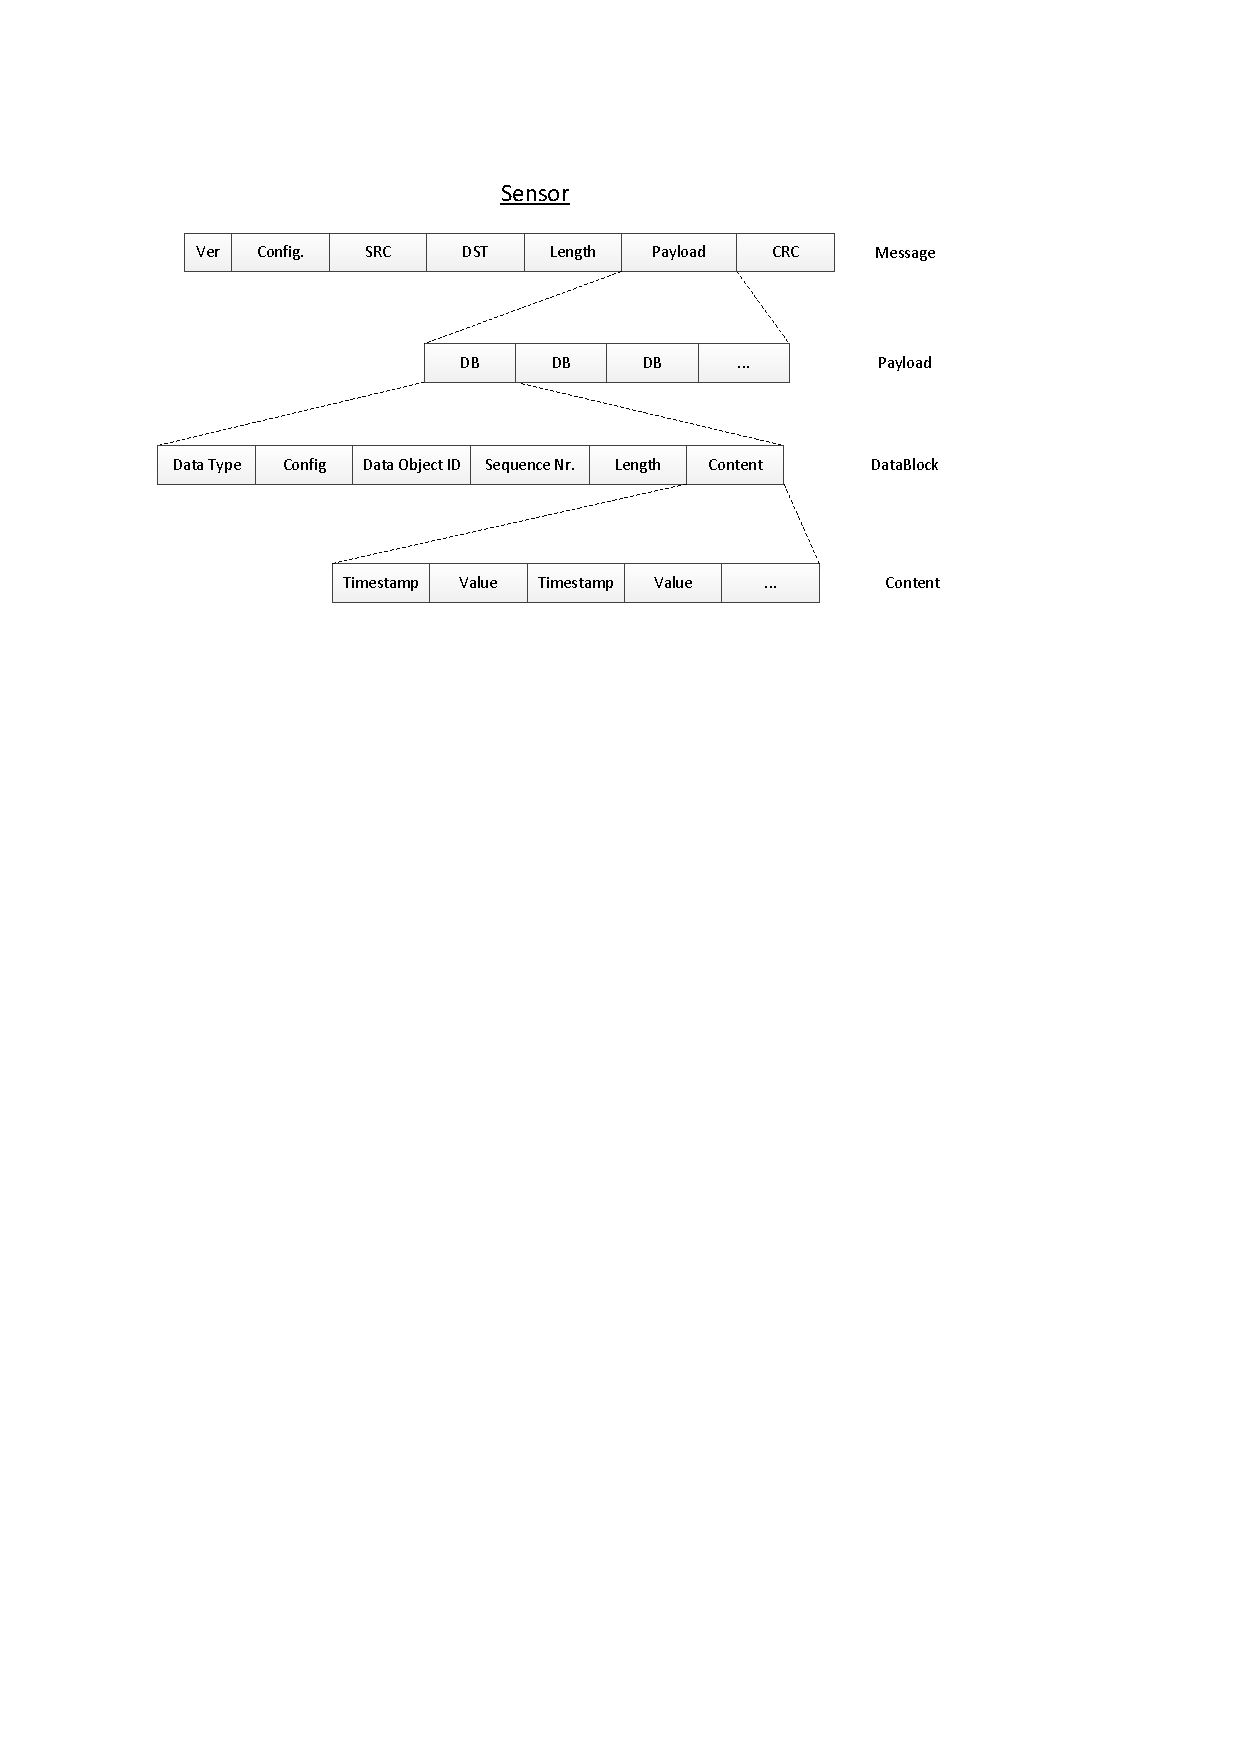
\includegraphics[width=\textwidth/2]{DatenaufschluesselungSensor.pdf}}\hfill
  \subfigure[Text]{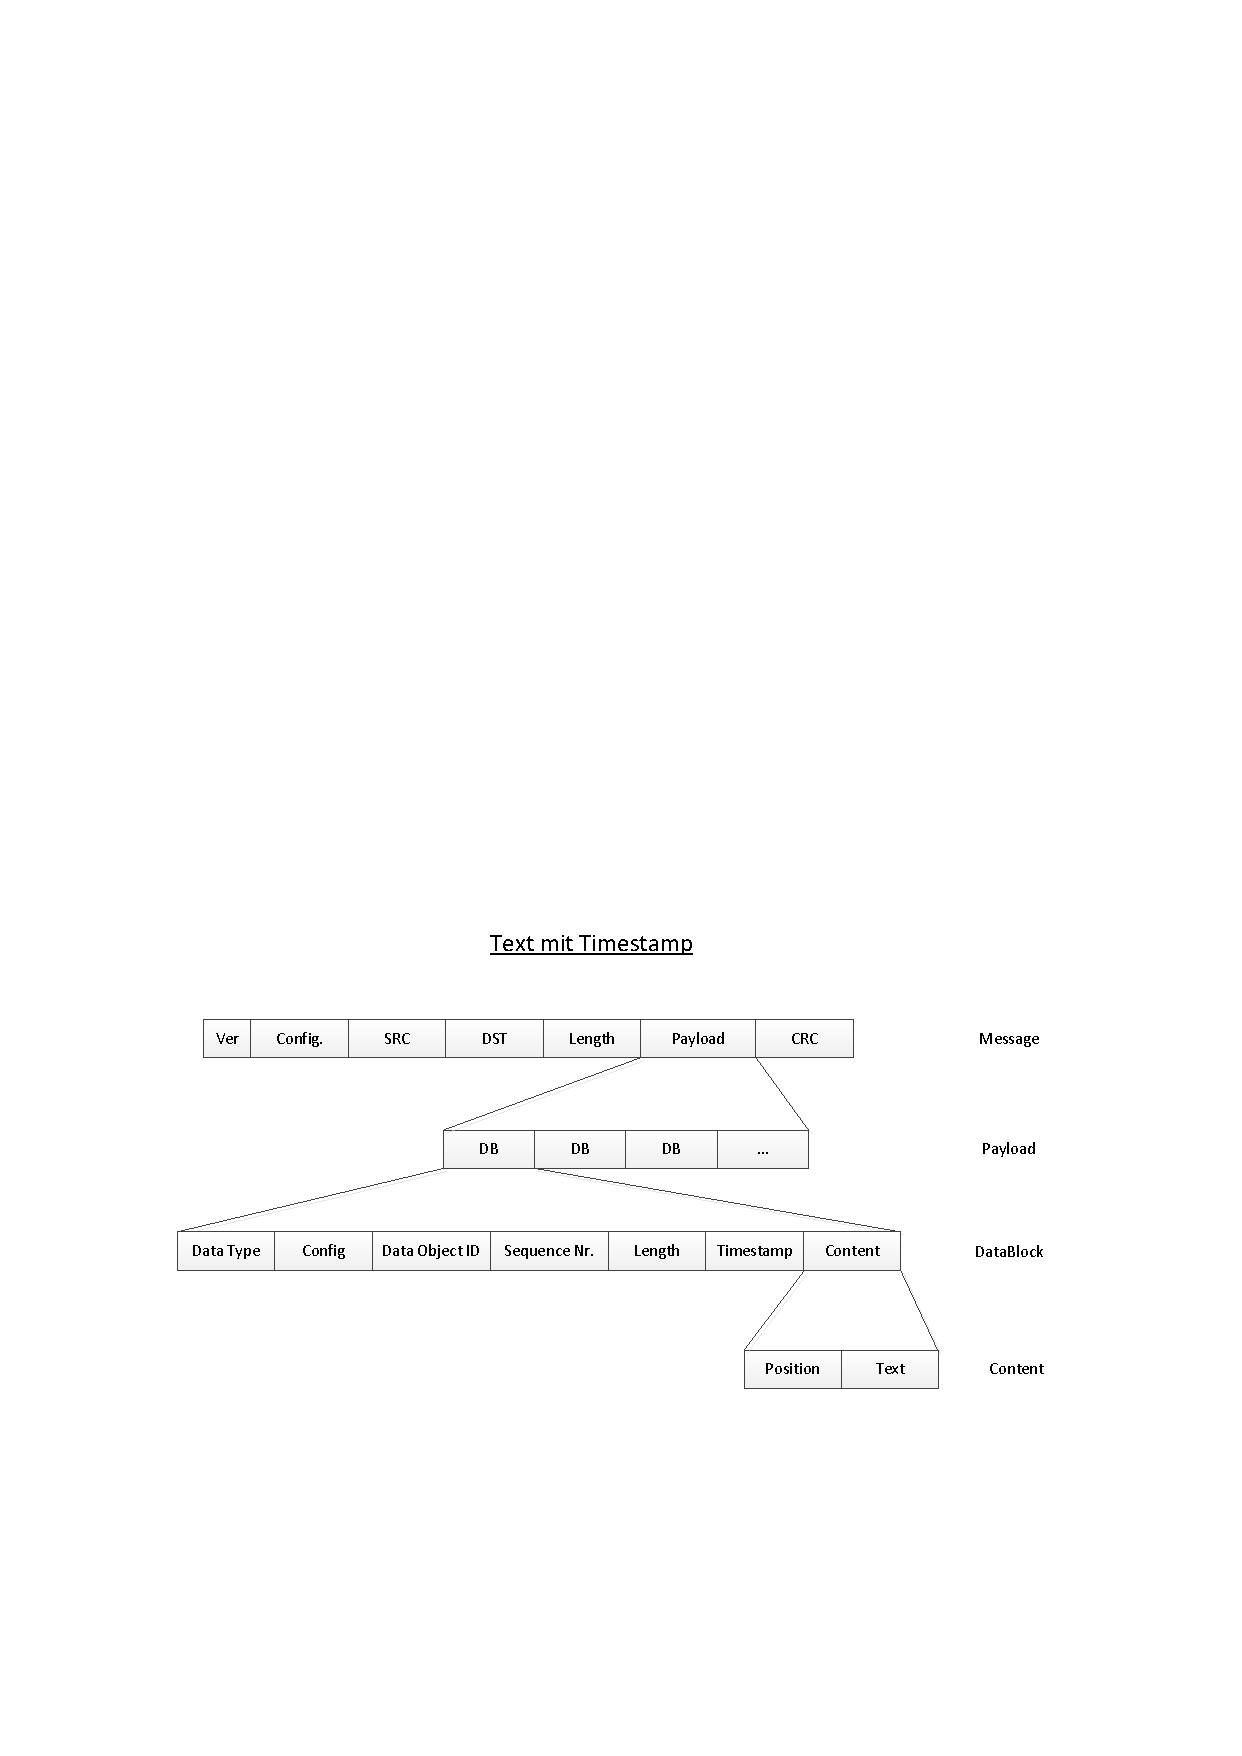
\includegraphics[width=\textwidth/2]{DatenaufschluesselungText.pdf}} 
  \caption{Übersicht der Datenaufschlüsselung}
  \label{fig:uebersichtdatenaufschluesselung}
\end{figure}

Durch den oben beschriebenen Aufbau wird eine flexible Handhabung
zahlreicher Datentypen ermöglicht. In Abbildung \ref{fig:beispielJPG} ist
dieser Vorgang anhand eines Bildes im Format JPEG dargestellt. Das Bild wird in mehrere
Datenblöcke zerlegt, welche die Bildinformationen (Content) beinhalten.
Diese wiederum bestehen aus einer Vielzahl an Pixeln.
Die Bildaten und der JPEG-Header bilden den Content. Ein Datenblock besteht
somit aus dem oben beschriebenen Content und dem dazugehörigen
Datenblockheader.

\begin{figure}[H]
	\centering
	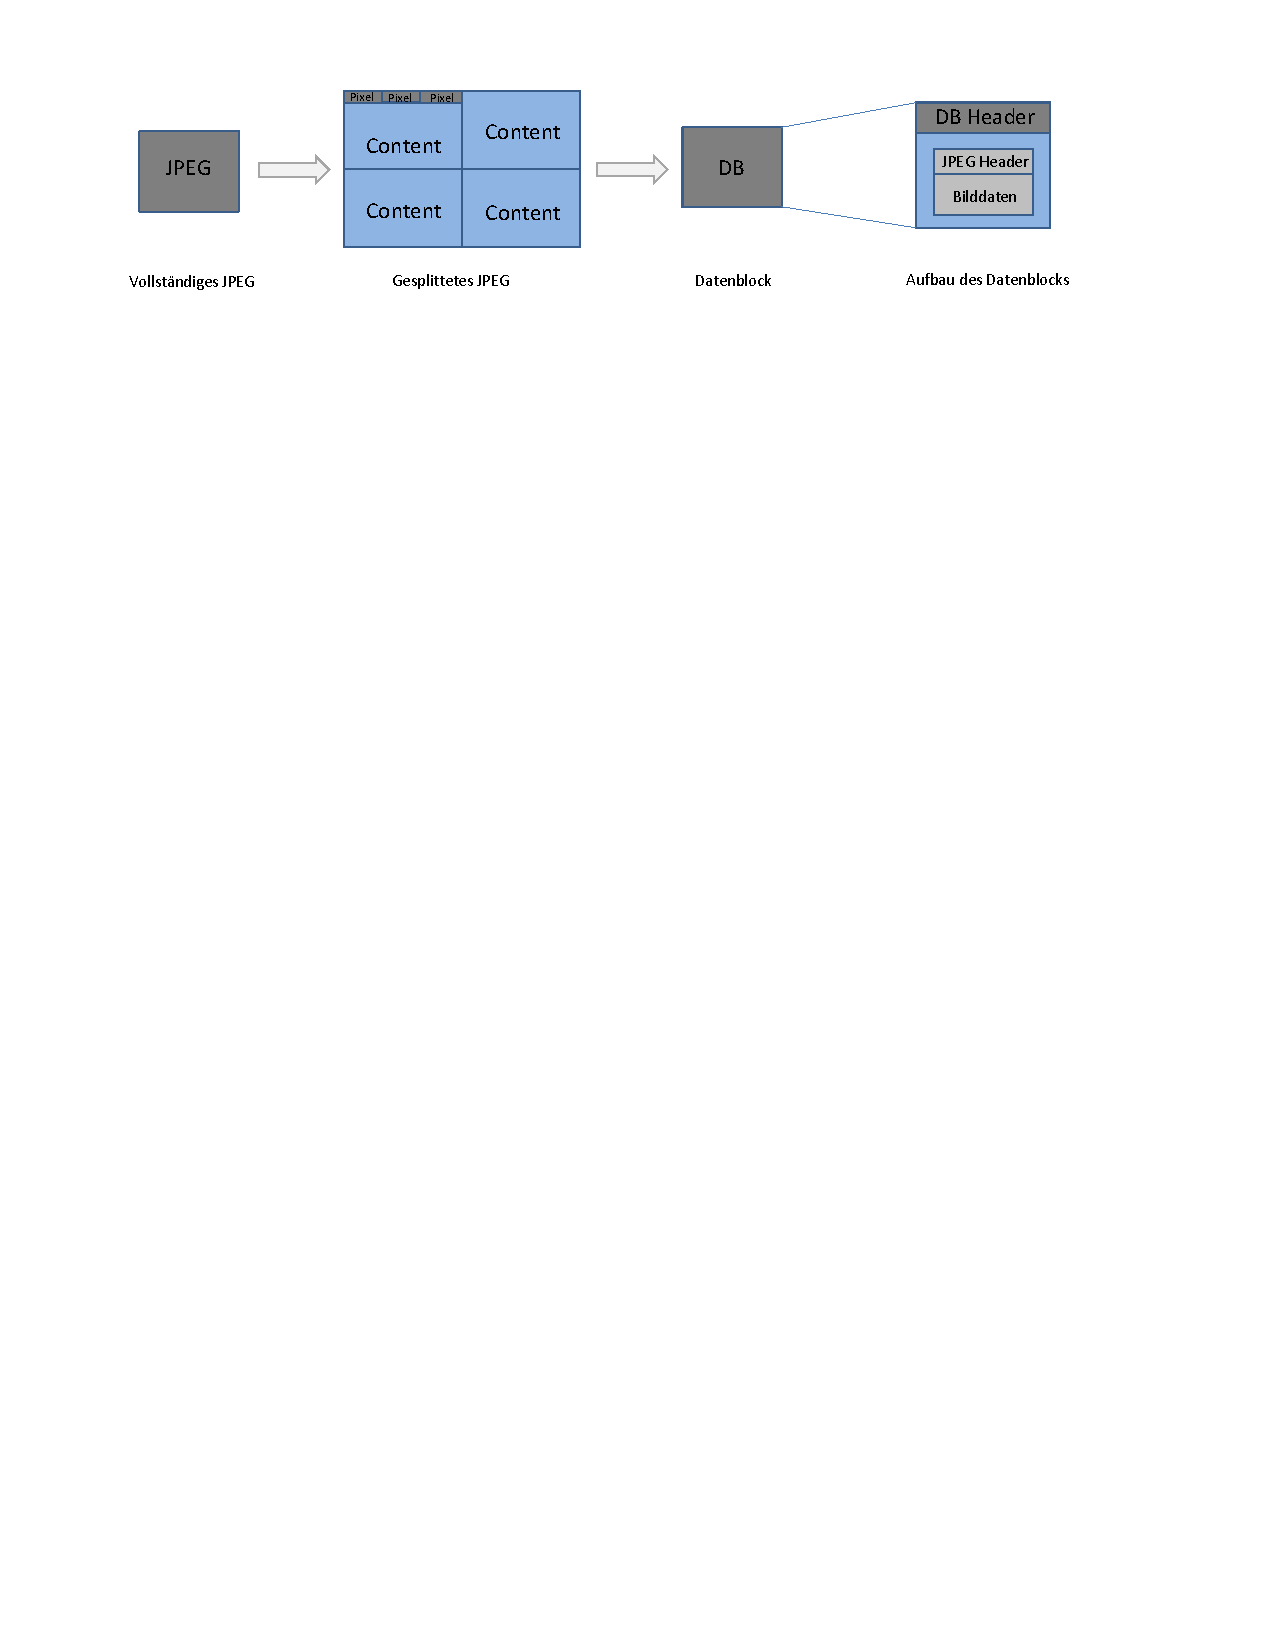
\includegraphics[width=\textwidth]{VerarbeitungJPEG-Bild.pdf}
	\caption{Verarbeitung eines JPEG-Bildes}
	\label{fig:beispielJPG}
\end{figure}

\textbf{Relevanz und Priorisierung}

Neben der Strukturierung und dem Aufbau der Nachricht selbst ist die
Wahl der Reihenfolge einzelner Datenblöcke sehr wichtig. Die Sortierung erfolgt
hierbei grundlegend in zwei Schritten, wie die Abbildung \ref{fig:priorisierungen}
zeigt.
Zunächst erfolgt eine Vorpriorisierung. Dabei werden relevante Bereiche
selektiert und mit einem Relevanzwert eingestuft. Die
Daten werden daraufhin in einzelne Blöcke zerlegt (siehe Abbildung
\ref{fig:priorisierungen} rechts) und erhalten abhängig ihrer Wichtigkeit einen
Prioritätswert. Danach erfolgt die Einsortierung der Datenblöcke unter
Berücksichtigung des Prioritätswertes in eine \gls{FIFO}.

\begin{figure}[H]
	\centering
	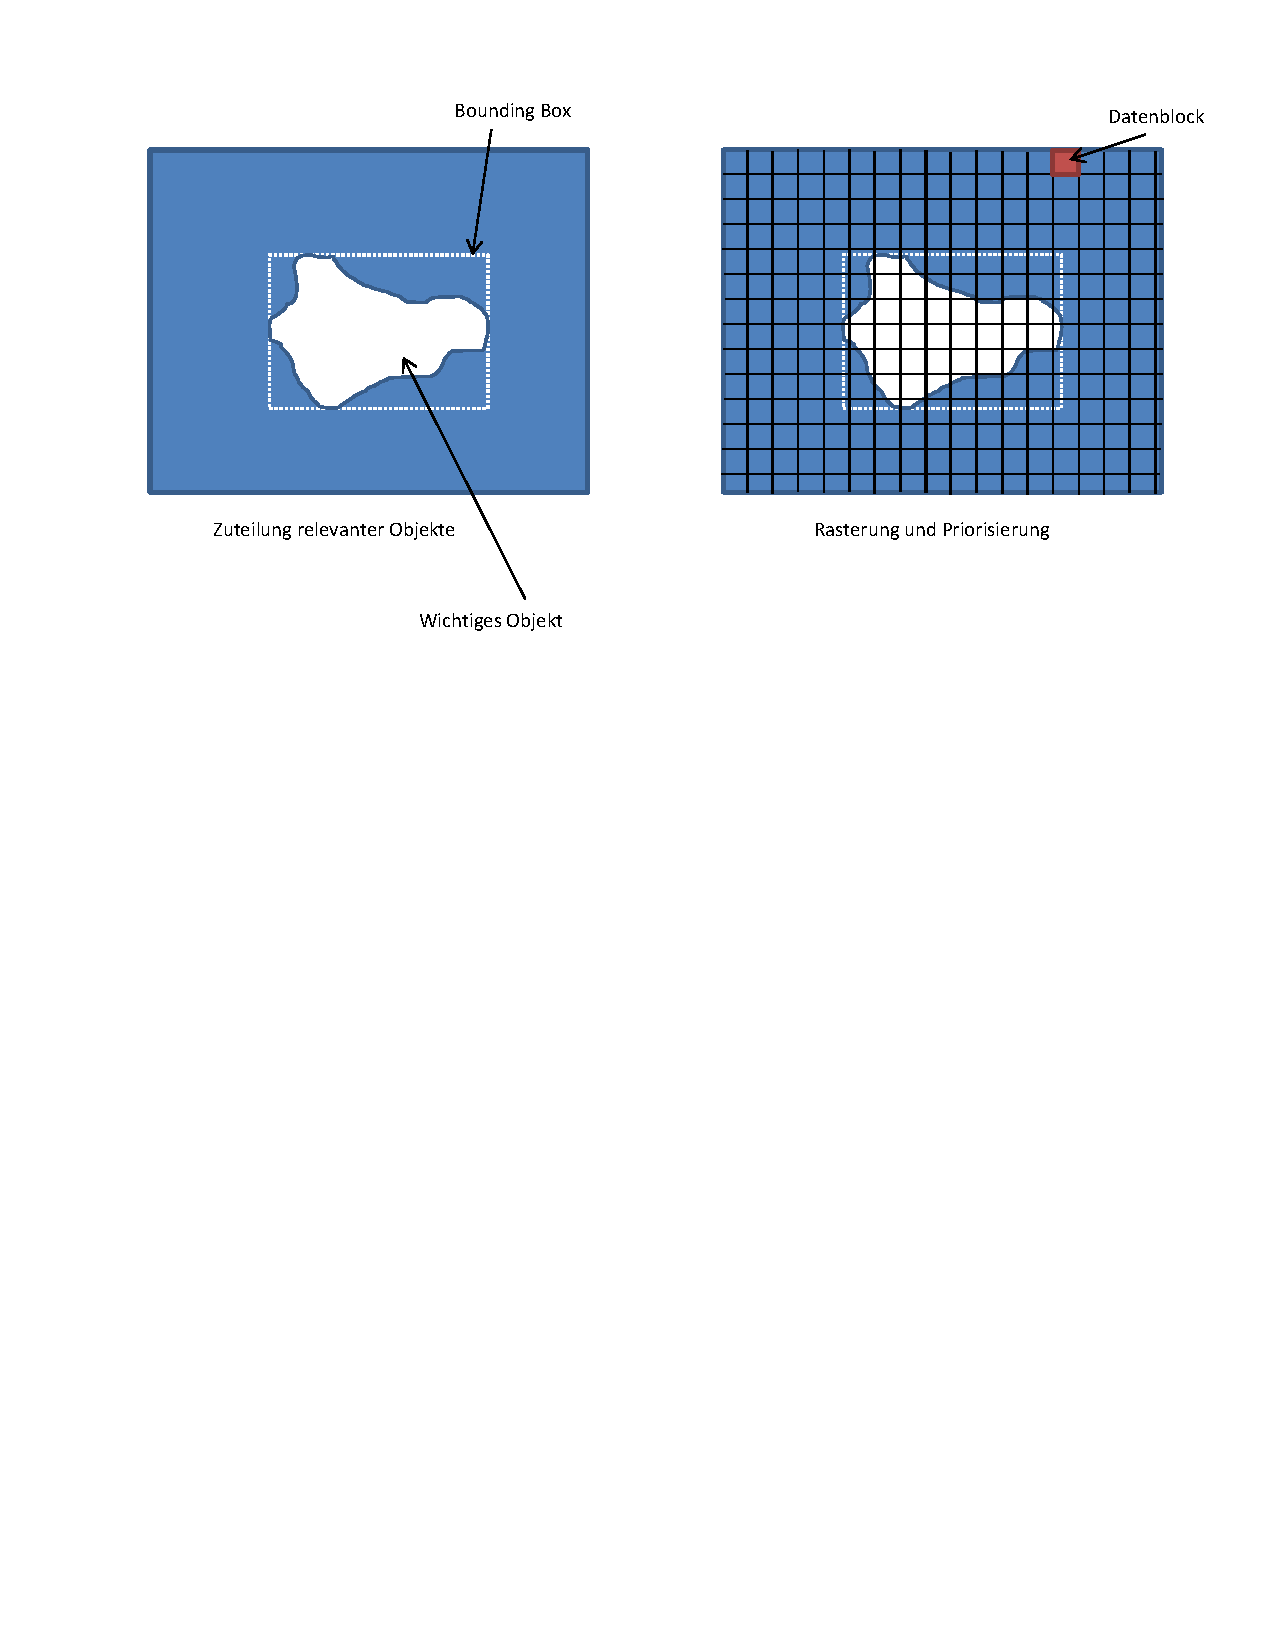
\includegraphics[width=\textwidth]{Priorisierung.pdf}
	\caption{Datenaufschlüsselung der Nachricht}
	\label{fig:priorisierungen}
\end{figure}

	\section{Anwendungsszenarien}
		\label{sec:Anwendungsszenarien}

Im Folgenden werden Anwendungsszenarien für das \gls{CROP} dargestellt. Dabei
wird die Funktionsweise sowohl anhand eines Textes als auch eines Bildes beschrieben und
verglichen. Dies erfolgt von der Eingabe über die Splittung bis hin zum Versand
der Nachricht.

Die Art und Weise wie ein Bild oder ein Text untersucht und bearbeitet wird
unterscheidet sich. Im Rahmen dieser Arbeit wird ein Text als
Anwendungsszenario herangezogen. Grundlage bildet hierbei eine Nachricht,
welche der Nutzer über eine grafische Benutzeroberfläche eingibt.
Dabei ist zusätzlich ein manuelles Hervorheben der wichtigen Textpassagen
notwendig. Zur näheren Erläuterung soll folgendes fiktives Testszenario zur
Betrachtung herangezogen werden:

\textit{\glqq Gestern um 8 Uhr Marszeit wurden Hinweise auf mögliches Leben auf
dem Mars entdeckt, wobei ein Mann schwer verletzt wurde! \grqq}

Die höchste Aufmerksamkeit gilt der Tatsache, dass mögliches Leben entdeckt und
dabei ein Mann schwer verletzt wurde. Demnach bekommen diese beiden Abschnitte
die höchste Priorität. Folgen könnte die Uhrzeit, damit der Empfänger zuordnen
kann, wie lange die Verletzung bereits vorliegt. Alle weiteren Wörter stellen
zusätzliche Informationen dar, die für die Vollständigkeit des Textes, aber
nicht zum Verständnis der Situation notwendig sind. Die Abbildung
\ref{fig:prioChatWindow} zeigt die Prioritäten in der ChatGui, auf die im
Kapitel \ref{cap:chatGui} noch näher eingegangen wird.

\begin{figure}[H]
	\centering
	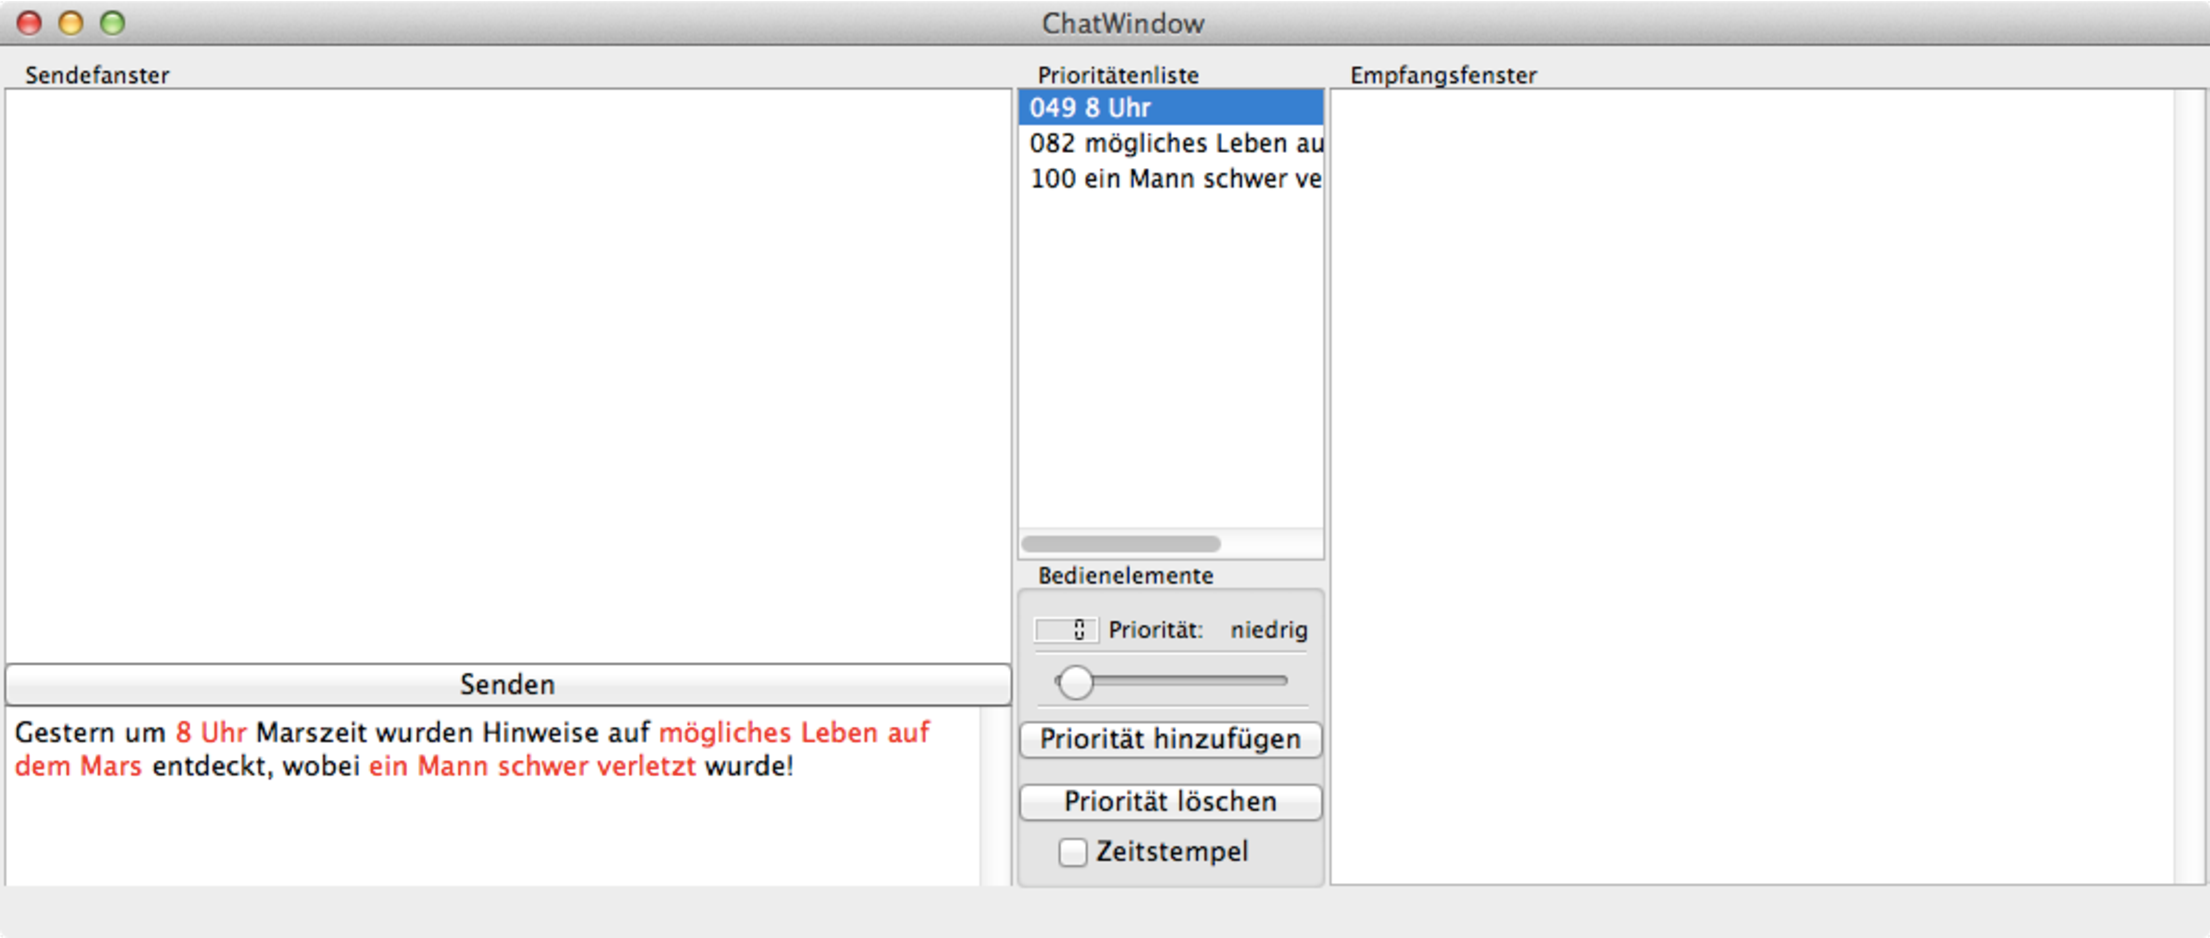
\includegraphics[width=\textwidth]{prioChatWindow.pdf}
	\label{fig:prioChatWindow}
	\caption{Chat-Fenster mit priorisierter Eingabe}
\end{figure}

Der Text wird jetzt Wort für Wort untersucht und anhand der Priorität sortiert.
Dabei bilden Wortgruppen mit gleicher Relevanz einen Datenblock, dem eine
Sequenznummer zugeordnet wird, wodurch eine eindeutige Identifizierung möglich
ist. Die \gls{DOID} beugt einer Verwechslung anderer Datenblöcke gleicher
Sequenznummer vor. Weiterhin werden die Position und die Länge der Wortgruppe im
Text abgespeichert. Anhand dieser Informationen ist der Empfänger in der Lage
die ankommenden Datenblöcke korrekt zuzuordnen und so den Text
wiederherzustellen.
In Abbildung \ref{fig:chatguiexample} ist dargestellt, wie einzelne Fragmente
zuerst ankommen und der Text mit jedem weiteren Datenpaket vervollständigt wird.

\begin{figure}[H]
	\centering
	\subfigure{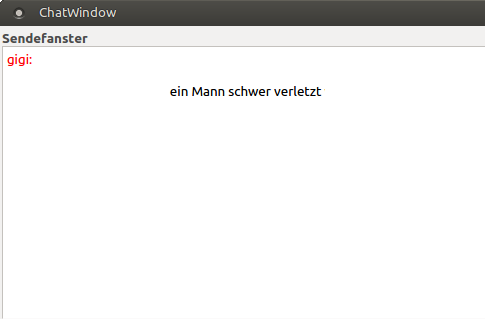
\includegraphics[scale=.6]{chatGuiWindow_empfaenger_prio.png}}\\
	\subfigure{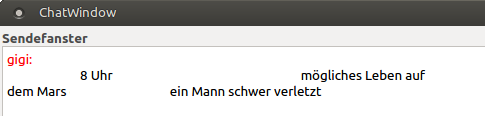
\includegraphics[scale=.6]{chatGuiWindow_empfaenger_halfPrio.png}}\\
	\subfigure{
\includegraphics[scale=.6]{chatGuiWindow_empfaenger_all.png}}
	\label{fig:chatguiexample}
	\caption{Wiederherstellung der Nachricht beim Empfänger}
\end{figure}

Der Ablauf eines Bildes gestaltet sich ähnlich. Die Abbildung
\ref{fig:marsWaterResidue} (a) zeigt das vom Marsrover \textit{Curiosity}
am $28.$ September aufgenommene ausgetrocknete Wasserbett. Der im
linken Bild markierte Bereich zeigt, Wissenschaftlern zufolge, einen vom Wasser
verformten Kiesel \cite{web11}. Wie beim Szenario zuvor erfolgt zunächst
eine Markierung der wichtigen Bereiche. Diese sind der Kiesel und der Maßstab, welche in der
Abbildung \ref{fig:marsWaterResidue} (b) dargestellt werden. Bevor das Bild
Schritt für Schritt analysiert wird, muss dieses in Abschnitte eingeteilt
werden, welche später die einzelnen Datenblöcke darstellen.
 
\begin{figure}[H]
	\centering
	\subfigure[Originalbild]{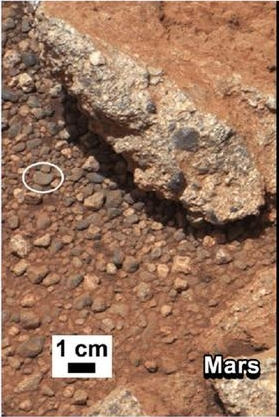
\includegraphics[scale=.4]{marsWaterResidue_links.jpg}}\hfill
	\subfigure[Markierung der Relevanz]
	 {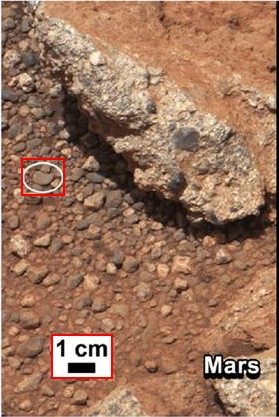
\includegraphics[scale=.4]{marsWaterResidue_mitte.jpg}}\hfill
	\subfigure[Zerlegung des Bildes]
	 {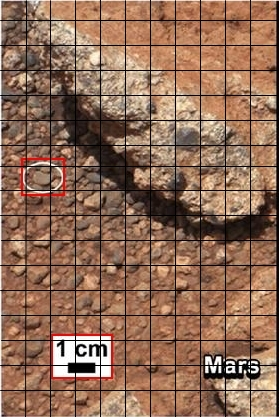
\includegraphics[scale=.4]{marsWaterResidue_rechts.jpg}}
	\label{fig:marsWaterResidue}
	\caption[Priorisierung des Bildes]{Priorisierung des Bildes \cite{img3}}
\end{figure}

Die weiteren Schritte sind equivalent zu denen des Textes. Die beiden wichtigen
und damit höher priorisierten Bereiche erreichen den Empfänger zuerst.
Das Zusammensetzen des Bildes wird in seiner prinzipiellen Form in
Abbildung \ref{fig:marsWaterResidueEmpfaenger} dargestellt.

\begin{figure}[H]
	\centering
	\subfigure[leeres Bild]
	 {
\includegraphics[scale=.4]{marsWaterResidue_empfaenger_links.jpg}}\hfill
	\subfigure[empfangene wichtige Bereiche]
	 {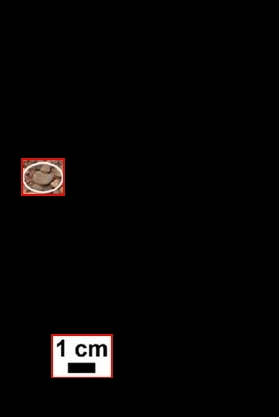
\includegraphics[scale=.4]{marsWaterResidue_empfaenger_mitte.jpg}}\hfill
	\subfigure[wieder zusammengesetztes Bild]
	 {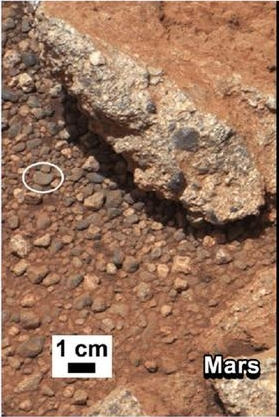
\includegraphics[scale=.4]{marsWaterResidue_empfaenger_rechts.jpg}}
	\label{fig:marsWaterResidueEmpfaenger}
	\caption{Wiederherstellung des Bildes}
\end{figure}
	\section{Schnittstellen}
		Anhand der im vorherigen Kapitel \ref{sec:Anwendungsszenarien} genannten Anwendungsszenarien lassen
sich die einzelnen Schnittstellen zwischen den Modulen ableiten. In
\abbildung{Schnittstellen} ist ein schematischer Aufbau der Module
dargestellt. Die Schnittstellen zwischen diesen sind nummerisch gekennzeichnet.

\begin{figure}[H]
\centering
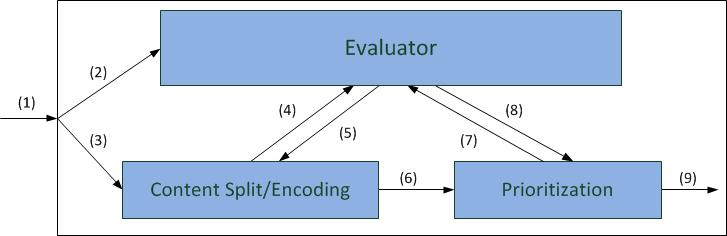
\includegraphics[scale=.7]{Schnittstellen.jpg}
\caption{Schnittstellen der Module}
\label{fig:Schnittstellen}
\end{figure}

Daraus ergeben sich die folgenden Verallgemeinerungen:

\textbf{Schnittstelle (1)}\newline
Die Schnittstelle (1) ist die Gesamtschnittstelle. Hier wird der
Content an das Modul übergeben. Weiterhin erfolgt die Übergabe der DOID, des
Datentypes und eines Flags, welches angibt, ob ein Zeitangabe berücksichtigt
werden soll.
Optional sind ein oder mehrere Positionsangaben mit einem Relevanzwert
anzugeben. Als Relevanzwert wurde festgelegt, dass dieser eine prozentuale
Angabe im Bereich von 0 bis 100 ist. Dabei wird 0 als unwichtig und 100 als
sehr wichtig eingestuft. Die Positionsangaben beinhalten zum einen den
Startpunkt des relevanten Bereiches mit einer x- und y-Koordinate. Weiterhin
wird das Volumen des Bereiches mit einer Länge in x- und y-Richtung angegeben.
Die Angabe der Positionen und des Relevanzwertes ist \zB notwendig, wenn diese
Daten nicht selbst berechnet werden sollen, sondern der Benutzer diese über eine
grafische Benutzeroberfläche vorgibt.

\textbf{Schnittstelle (2)} \newline
An den Evaluator wird von den Eingangsdaten der Schnittstelle (1)
der Content übergeben. Zusätzlich werden die Relevanzwerte mit den
Positionsangaben übermittelt, wenn diese vorgegeben wurden.

\textbf{Schnittstelle (3)} \newline
Aus Schnittstelle (1) wird an die Partitonierung
die DOID, der Datentyp, der Content und das Zeitflag weitergegeben.

\textbf{Schnittstelle (4)} \newline
Damit der Evaluator nachvollziehen kann, welches Datenpacket gerade bearbeitet
wird, erfolgt die Übergabe der DOID und des Datentyps.  

\textbf{Schnittstelle (5)} \newline
Als Antwort auf die einkommenden Daten der Schnittstelle (4)
erfolgt die Rückgabe der relevanten Bereiche mit den Positionen und den
dazugehörigen Relevanzwerten durch den Evaluator.

\textbf{Schnittstelle (6)} \newline
Nach der Zerlegung der Blöcke werden die einzelnen
Datenblöcke mit den dazugehörigen Datenblockheadern an die
Priorisierung übergeben.

\textbf{Schnittstelle (7)} \newline
Durch Übergabe der DOID, des Datentypes und der Positionsangaben kann der
Content identifiziert werden.

\textbf{Schnittstelle (8)} \newline
Durch erhalt der Daten in Schnittstelle (7) kann für
den Datenblock eine Priorität berechnet werden, welche an die Priorisierung übergeben
wird. Die Priorität wird als reelle Zahl aufgefasst und ist ähnlich des
Relevanzwertes eine prozentuale Größe zwischen 0 und 100.

\textbf{Schnittstelle (9)} \newline
Nach der Priorisierung werden die priorisierten Datenblöcke mit den
Datenblockheadern und der Priorität an die Packetization übergeben.

Bei den Schnittstellen ist zu beachten, dass manche Angaben abhängig von den
jeweiligen Datentypen sind und für den Fall nicht benutzt oder
standardmässig auf einen bestimmten Wert gesetzt werden. Beispielsweise benötigt
ein Text als Positionsangaben keine Länge in y-Richtung. Dieser ist bei einem
Bild jedoch zwingend notwendig.


\chapter{Implementierung}
	\label{cap:implementierung}
F{\"u}r die Umsetzung der im Kapitel \ref{cap:konzept} angesprochenen Ideen und
Eigenschaften wurde die Programmiersprache C++ verwendet, welche eine
Erweiterung der Programmiersprache C ist. Das Betriebsystem VxWorks ist in der
Programmiersprache C geschrieben, dass beispielsweise auf dem Mars Rover
\textit{Curiosity} eingesetzt wird \cite{WR}.
Als Entwicklungsumgebung kam Eclipse zum Einsatz.
Zur Verbesserung der Teamarbeit und des Austausches von Quellcode wurde ein
Github Repository \footnote{www.github.com} angelegt, welches {\"u}ber das
Eclipse-Plugin EGit genutzt wurde. \newline
Im Folgenden wird im Detail auf die Art und Weise der Realisierung der beiden
Top-Level-Module \Code{Sender} und \Code{Receiver} eingegangen. Hierf{\"u}r
wurde eine flexible und modulare Softwarearchitektur entwickelt, damit auf
sp{\"a}tere {\"A}nderungen, neue Anforderungen und erforderliche Optimierungen
reagiert werden kann. Dies ist durch das einfache Austauschen kompletter Module
m{\"o}glich.
Daf{\"u}r wird ein objektorientiertes Design genutzt, womit Quellcoderedundanzen und damit
zahlreiche potentielle Programmierfehler vermieden werden konnten.
Weiterhin ist die Wiederverwendung einzelner Quellcodepassagen m{\"o}glich.\newline
Damit die beiden Module in anderen Projekten einfach genutzt werden k{\"o}nnen,
wurde eine statische Bibliothek erstellt, welche {\"u}ber eine Schnittstelle die
Funktionen der beiden Module bereitstellt. In dieser Arbeit wurden nur die beiden
Datentypen Text und Sensorwerte integriert.

\section{Modulaufbau Sender}
 
Die Aufgabe des Moduls \Code{Sender} besteht darin, die aus vier Phasen
bestehende Verarbeitung der Daten umzusetzen \cite{Daher}.
In Abbildung \ref{fig:BlockdiagrammSender} ist das Blockdiagramm und im Anhang
\ref{fig:KlassendiagrammSender} das dazugehörige Klassendiagramm des Moduls
\Code{Sender} dargestellt.
Dies bietet eine {\"U}bersicht zu den Modulen und zeigt wie diese untereinander 
kommunizieren. In der Grafik ist jedes Submodul durch ein M in der linken
oberen Ecke des Blockes gekennzeichnet. Ebenso ist die Schnittstellenklasse
angegeben und durch die Abk{\"u}rzung \gls{IF} gekennzeichnet. Dadurch ist der
geforderte modulare Aufbau sichergestellt.

\begin{figure}[H]
\centering
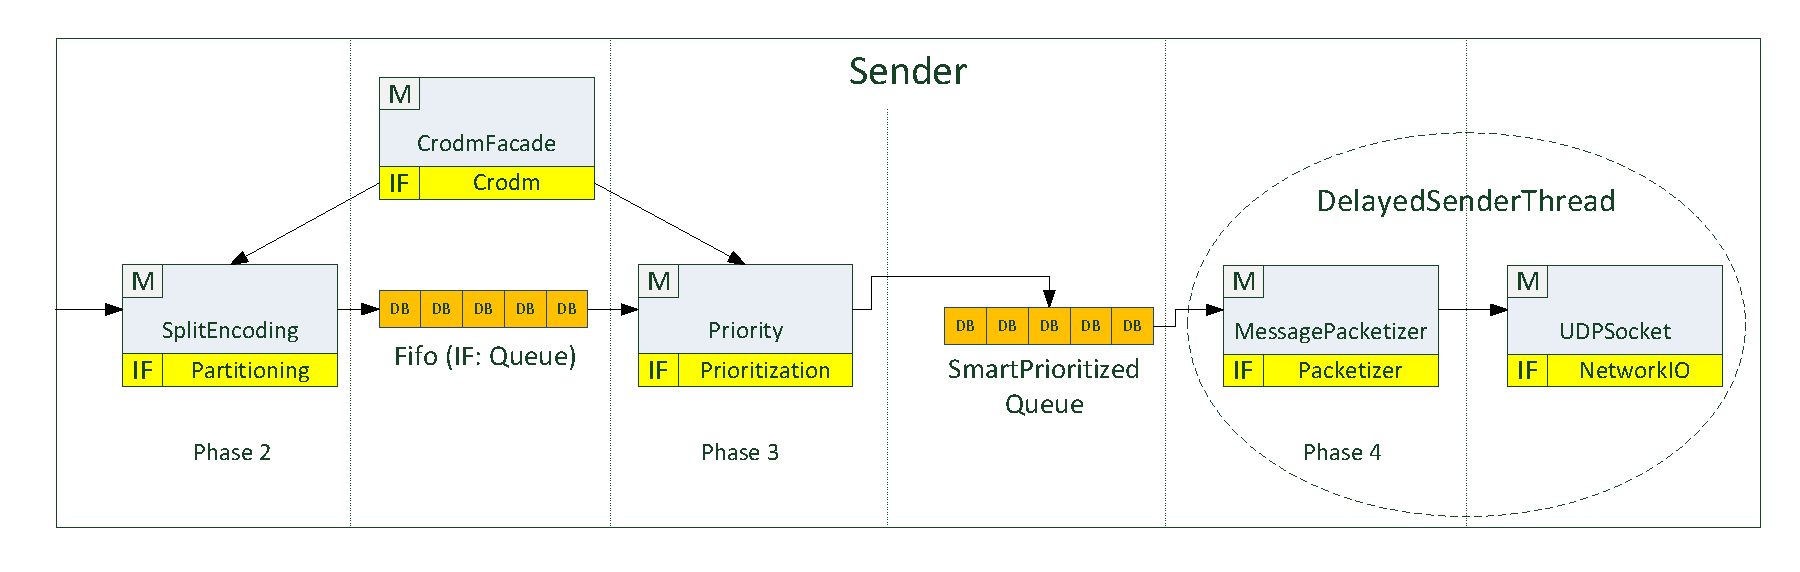
\includegraphics[scale=.49]{BlockdiagrammSender.pdf} % skalieren
\caption{Blockdiagramm des Senders}
\label{fig:BlockdiagrammSender}
\end{figure}

Die Daten werden {\"u}ber die Schnittstelle des Topmoduls \Code{Sender}
{\"u}bergeben und an die Klasse \Code{Partitionierung} weitergegeben. Dort
werden diese, abh{\"a}ngig von ihrer Relevanz, in Datenbl{\"o}cke zerlegt.
Zus{\"a}tzlich werden in diesem Schritt die Datenblockheader (siehe Kapitel
\ref{sec:ProtokolDesign}) erstellt und der Content in bin{\"a}re Daten
umgewandelt. Am Ende werden die Datenbl{\"o}cke mit den Headerinformationen in
einer \gls{FIFO} gepuffert.
Anschließend wird jedem einzelnen Datenblock im n{\"a}chsten Modul eine
Priorit{\"a}t zugewiesen. Die angesprochene Relevanz und die Priorit{\"a}t der
Datenbl{\"o}cke werden in einem extra Modul namens \gls{CRODM} berechnet oder
manuell durch den Nutzer zugewiesen und anschließend dem Modul \Code{Priority}
{\"u}bergeben.
Anhand dieser wird der Datenblock in die Datenstruktur
\Code{SmartPrioritizedQueue} einsortiert. Dadurch wird gew{\"a}hrleistet, dass
die wichtigen Daten zuerst gesendet werden. F{\"u}r diese Aufgabe wird eine
einfache Liste aus der \gls{STL} verwendet. Durch diese kann iteriert werden und
es besteht ein schneller zufälliger Zugriff auf jedes Element, welches nun
ebenso effektiv eingefügt und gelöscht werden kann.
Weiterhin exsistiert die notwendige Sortierfunktion. Diese hat f{\"u}r den durch sie
ausgef{\"u}hrten Zweck eine vergleichsweise gute Laufzeit.
Damit die Verz{\"o}gerung, die durch gro{\ss}e Entfernungen auftritt, besser
ber{\"u}cksichtigt werden kann, wird das Submodul \Code{Packetizer} als Thread
gestartet.
Dieser holt sich die Pakete mit der h{\"o}chsten Priorit{\"a}t aus der
\Code{SmartPrioritizedQueue} und verpackt diese in eine Nachricht, welche
anschlie{\ss}end an die Netzwerkschnittstelle {\"u}bergeben und versandt wird.
\newline Die Umsetzung der Submodule wird im Folgenden genauer
erl{\"a}utert.

\subsection{Splitten und Encoden}

Die Aufgabe des Submoduls \Code{SplitEncoding} ist es, die einkommenden Daten
anhand ihrer Relevanz in kleine Datenbl{\"o}cke zu unterteilen. F{\"u}r die Entwicklung
des daf{\"u}r erforderlichen Algorithmus wurde der in
Abbildung \ref{fig:Beispieltext} dargestellte Beispieltext erstellt.

\begin{figure}[H]
	\centering
	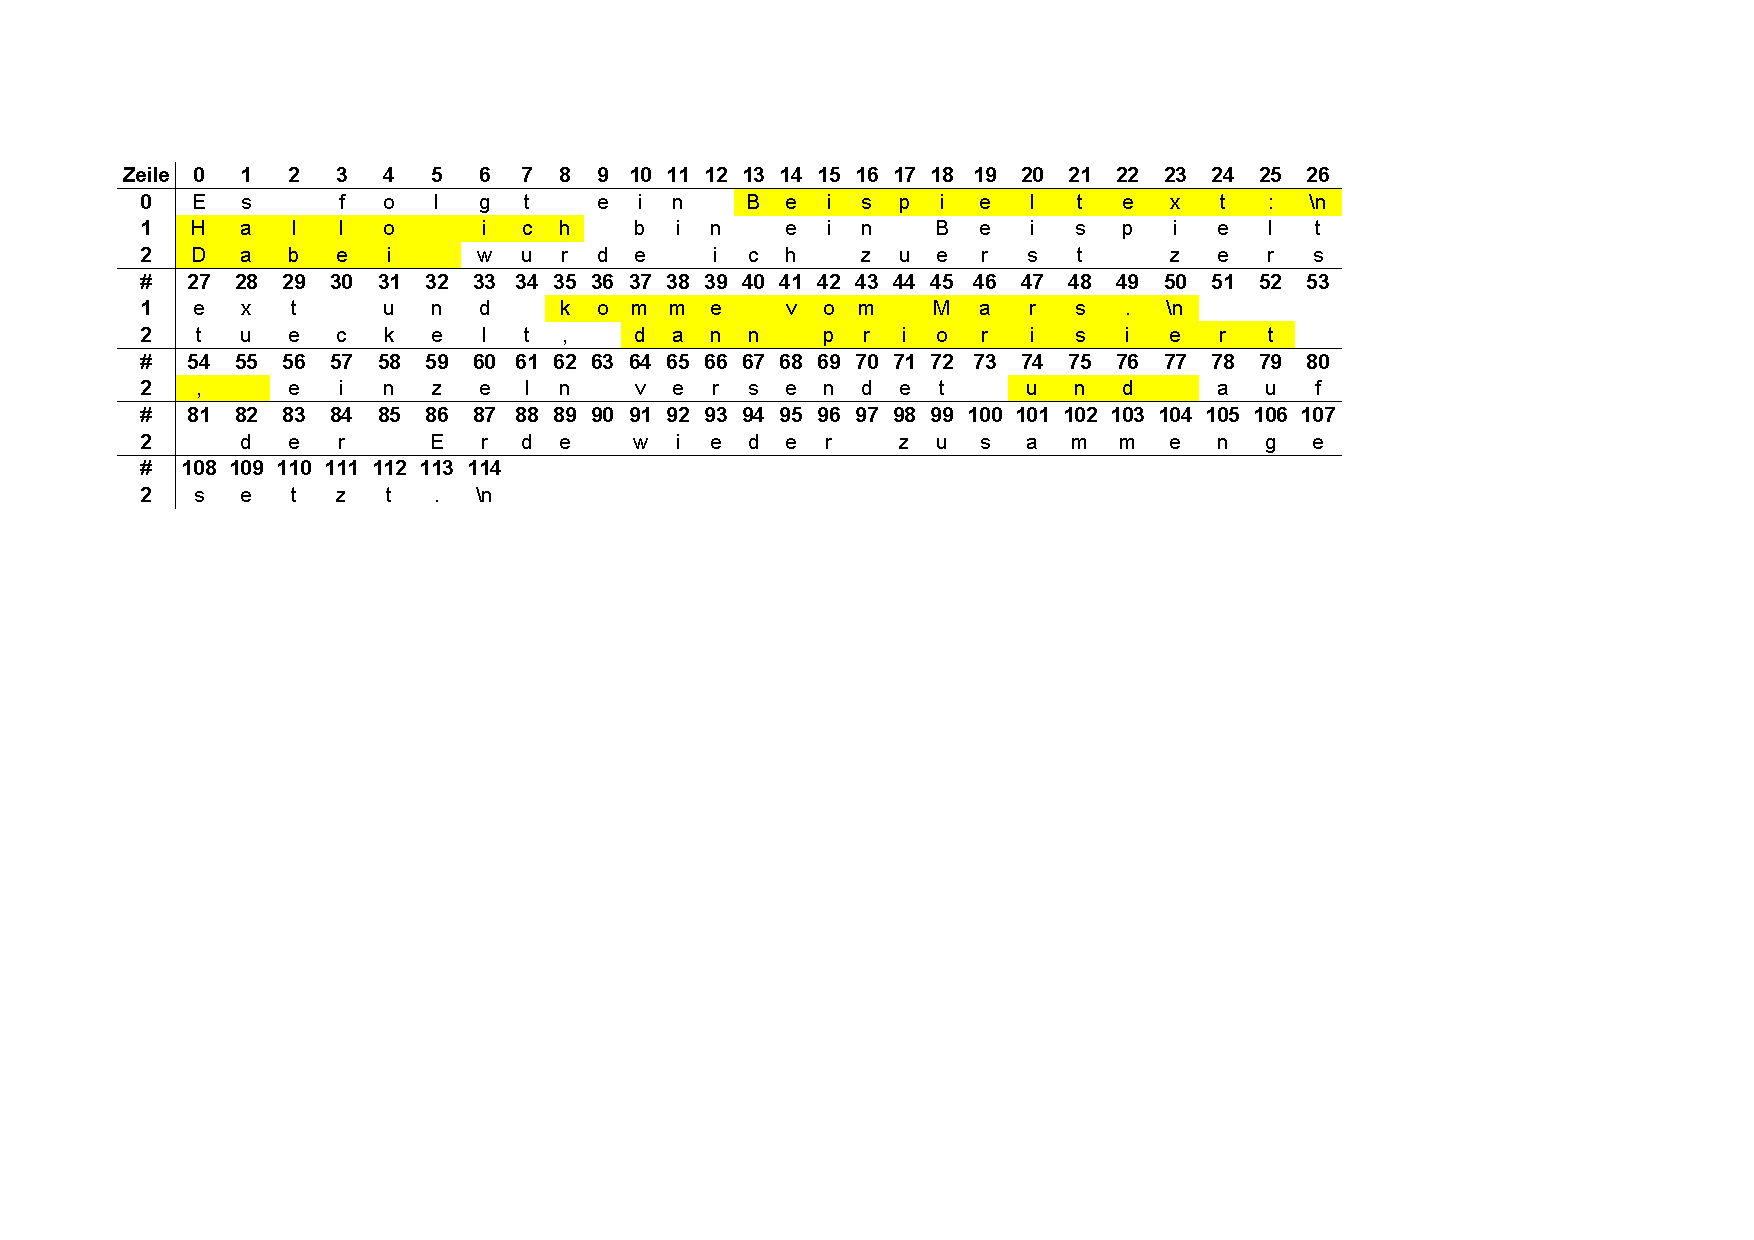
\includegraphics[scale=.6]{Beispieltext.pdf}
	\caption{Beispieltext}
	\label{fig:Beispieltext}
\end{figure}

In diesem Testfall wurden die relevanten Bereiche willk{\"u}rlich festgelegt, mit
dem Augenmerk m{\"o}gliche Randf{\"a}lle abzudecken. Die relevanten Bereiche sind in
der Abbildung \ref{fig:Beispieltext} gelb markiert.\newline
Daraus ergeben sich folgende Positionen der relevanten Bereiche:

\begin{longtable}{|cccl|}
	\caption{{\"U}bersicht der relevanten 2D-Bereiche} \\
	\hline
	\label{tab:UebersichtDerRelevantenBereiche}
	\textbf{x-Position} & \textbf{y-Position} & \textbf{x-L{\"a}nge} &
	\textbf{relevanter Text}\\
	\hline
	  13 &  0 & 14 & "`Beispieltext:\ensuremath{\backslash}n"' \\
	   0 &  1 &  9 & "`Hallo ich"' \\
	  35 &  1 & 22 & "`komme vom Mars.\ensuremath{\backslash}nDabei"' \\
	  37 &  2 & 18 & "`dann priorisiert,"' \\
	  73 &  2 &  4 & "`und "' \\
	\hline
\end{longtable}

F{\"u}r den Algorithmus ist es wichtig, dass die relevanten Bereiche den
Positionen nach sortiert sind. Das bedeutet, je niedriger die Zeile und Spalte,
desto weiter vorn ist diese Position in der Datenstruktur gespeichert.
Deshalb werden alle Angaben, die von dem Submodul \Code{CRODM}
{\"u}bergeben werden, zuerst sortiert.
Im n{\"a}chsten Schritt werden die zweidimensionalen Koordinaten zu einer
eindimensionalen umgerechnet, dadurch konnte das Herausschneiden der
Textfragmente, welche Zeilenspr{\"u}nge beinhalten k{\"o}nnen oder {\"u}ber eine
Zeile hinaus gehen k{\"o}nnen, vereinfacht werden. Daf{\"u}r
werden zuerst die akkumulierten Gesamtl{\"a}ngen der einzelnen Zeilen berechnet.
Vorhandene Umlaute und andere Zeichen, die nicht im
\gls{ASCII}\footnote{\gls{ASCII} ist eine 7-Bit Zeichencodierung.}-Zeichensatz
enthalten sind, ben{\"o}tigen die doppelte L{\"a}nge. Die Gesamtl{\"a}ngen der
Zeilen sind in der Tabelle \ref{tab:UebersichtDerAkkumuliertenZeilenlaengen}
angegeben.

\begin{longtable}{|cc|}
\caption{{\"U}bersicht der akkumulierten Zeilenl{\"a}ngen} \\
\hline
\label{tab:UebersichtDerAkkumuliertenZeilenlaengen}
\textbf{Zeile} & \textbf{L{\"a}nge}\\
\hline
  0 &    0 \\
  1 &   27 \\
  2 &   78 \\
  3 &  192 \\
\hline
\end{longtable}

Daraus ergeben sich die folgenden eindimensionalen Positionsangaben:

\begin{longtable}{|ccl|}
\caption{{\"U}bersicht der relevanten 1D-Bereiche} \\
\hline
\label{tab:UebersichtDerEindimensionalenBereiche}
\textbf{x-Position} & \textbf{x-L{\"a}nge} &
\textbf{relevanter Text}\\
\hline
   13 & 14 & "`Beispieltext:\ensuremath{\backslash}n"' \\
   27 &  9 & "`Hallo ich"' \\
   62 & 22 & "`komme vom Mars.\ensuremath{\backslash}nDabei"' \\
  115 & 18 & "`dann priorisiert,"' \\
  151 &  4 & "`und "' \\
\hline
\end{longtable}

Die Bl{\"o}cke f{\"u}r die relevanten Bereiche k{\"o}nnen genutzt werden,
um die dazwischenliegenden irrelevanten Fragmente zu berechnen. Die Differenz
zwischen der Endposition des ersten Blockes und der Anfangsposition des
darauf Folgenden ergibt die L{\"a}nge des neuen Blockes. Die Anfangspositon des
neuen Blockes ist die Endposition des Vorhergehenden. Die Relevanz ist Null.
Zusammengefasst ergibt die Berechnung die in Tabelle
\ref{tab:UebersichtDerUNRelevantenBereiche} aufgef{\"u}hrten Bereiche.

\begin{longtable}{|ccl|}
\caption{{\"U}bersicht der irrelevanten Bereiche} \\
\hline
\label{tab:UebersichtDerUNRelevantenBereiche}
\textbf{x-Position} & \textbf{x-L{\"a}nge} &
\textbf{unrelevanter Text}\\
\hline
   0 & 13 & "`Es folgt ein "' \\
  36 & 26 & "` bin ein Beispieltext und "' \\
  84 & 31 & "`wurde ich zerst{\"u}ckelt, "' \\
 133 & 18 & "`einzeln versendet "' \\
 155 & 37 & "` auf der Erde wieder zusammengesetzt.\ensuremath{\backslash}n"' \\
\hline
\end{longtable}

Zum Schluss muss noch der letzte Block berechnet werden, der nach dem letzten
relevanten Bereich {\"u}brig ist, falls dieser nicht mit dem Ende abschließt. Mit
diesen Daten kann der Teiltext f{\"u}r jeden Block aus dem Content
herrausgeschnitten werden. An dieser Stelle wird noch {\"u}berpr{\"u}ft, ob der
Datenblock des Teiltextes gr{\"o}{\ss}er ist als die maximale
Datenbl{\"o}ckgr{\"o}{\ss}e und ob dieser gegebenenfalls in mehrere kleinere
Teile zerlegt werden muss. Dieser wird danach zusammen mit den Informationen des Datenblockheaders in der Klasse \Code{Datablock}
gespeichert und in einer einfachen \gls{FIFO} hinterlegt. F{\"u}r die Sensorwerte
ist kein Zerlegen der Daten in Teilbl{\"o}cke notwendig.
Hier werden lediglich mehrere Daten einer Quelle mit dem passenden
Zeitstempel gebuffert, damit diese platzsparender in dem Datenblock als
Content eingef{\"u}gt werden k{\"o}nnen. \newline
Der Algorithmus ist noch einmal im nachfolgenden Pseudocode dargestellt.

\lstdefinelanguage{pseudo}{
morekeywords={if, else, for, in, remove, from, case, do, forever, to, false,
function, then, end, true, while}, sensitive=true,%
morecomment=[l]\#,%
morestring=[b]',%
}
\lstset{language=pseudo}
\lstset{commentstyle=\textit}
\lstset{literate=
 {<=} {$\le$}{2} {!=} {$\neq$}{2} {=} {$\leftarrow$}{2} {==} {=}{2} {&&}
{$\cap$}{2} {||} {$\cup$}{2} }
\lstinputlisting[label=PseudocodeSplitEncoding,
caption=Pseudocode des Moduls SplitEncoding] {Listings/PseudocodeSplitEncoding.txt}

\subsection{Verpacken}

Die priorisierten Datenbl{\"o}cke werden in diesem Schritt zu einer Nachricht
verpackt. Hierbei ist darauf zu achten, dass die maximale Paketgr{\"o}{\ss}e
nicht {\"u}berschritten wird. Weiterhin soll kein Platz verschwendet werden,
\dahe die Nachricht soll die maximale Nachrichtenl{\"a}nge so genau wie
m{\"o}glich erreichen.
Um die Nachricht auf der Empf{\"a}ngerseite wieder korrekt darstellen zu k{\"o}nnen, ist
die Einhaltung der Reihenfolge von gro{\ss}er Wichtigkeit. \newline
Das Submodul ist, wie bereits angesprochen, nebenl{\"a}ufig zum Programmablauf
integriert, um die Verz{\"o}gerungen simulieren zu k{\"o}nnen. Damit die
dadurch auftretenden Probleme der Gleichzeitigkeit vermieden werden k{\"o}nnen,
wurden Semaphore in die Klasse \Code{SmartPrioritizedQueue}
eingef{\"u}gt, welche sicherstellen, dass nicht zwei Programmteile gleichzeitig auf
die gleichen Daten zugreifen. Da erst am Ende bekannt ist, wie lang die
Nachricht sein wird, werden alle Daten zuerst tempor{\"a}r angelegt, die
L{\"a}nge addiert und zum Schlu{\ss} zur Nachricht zusammengef{\"u}gt.
Um die Nachricht m{\"o}glichst effizient zu verpacken, wird in der
Datenstruktur \Code{SmartPrioritizedQueue} zuerst das vorderste Paket
(\^= h{\"o}chste Priorit{\"a}t) herausgenommen. Deshalb wurde der
\Code{SmartPrioritizedQueue} eine gewisse Intelligenz integriert.
Diese ist in der Lage den Block mit der h{\"o}chsten Priorit{\"a}t zu finden, welcher
noch in den vorhandenen freien Raum der Nachricht passt. Dies stellt die
optimale L{\"o}sung dar, um den Platz sinnvoll aufzuf{\"u}llen. \newline 
Ist das erste Paket gr{\"o}{\ss}er als die maximale Nachrichtengr{\"o}{\ss}e,
f{\"u}r die ein CRC-16 genutzt werden kann, wird ein CRC-32 verwendet und die
Nachricht mit weiteren Datenbl{\"o}cken aufgef{\"u}llt, bis die maximale
Paketgr{\"o}ße erreicht ist. Dabei wird die Datenstruktur
\Code{SmartPrioritizedQueue} solange durchlaufen, bis kein Paket mehr vorhanden
ist, welches den noch freien Raum ausf{\"u}llen k{\"o}nnte. \newline 
Der Algorithmus ist in Abbildung \ref{fig:AlgorithmusPacketizer} graphisch
dargestellt.

\begin{figure}[H]
\centering
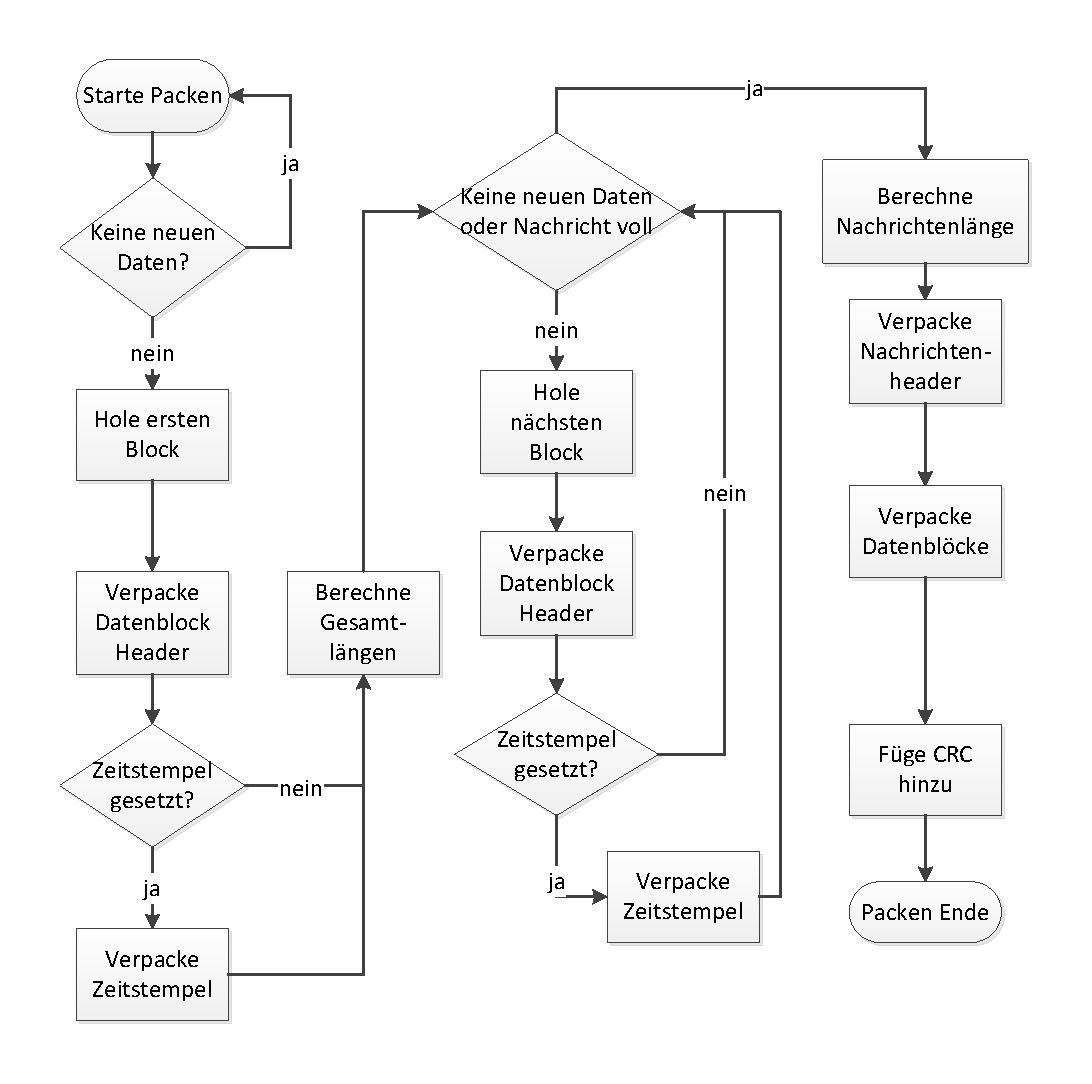
\includegraphics[scale=.6]{AlgorithmusPacketizer.pdf}
\caption{Algorithmus Packetizer}
\label{fig:AlgorithmusPacketizer}
\end{figure}

\subsection{Netzwerk}

Als Netzwerkschnittstelle wird ein \gls{UDP} Socket verwendet. Dieser erh{\"a}lt die
erstellte Nachricht vom Submodul \Code{Packetizer} und leitet diese an einen
zuvor ge{\"o}ffneten \gls{UDP} Socket weiter. Durch eine Client/Server basierte
Socket-Kommunikation {\"u}ber \gls{UDP} (verbindungslose Kommunikation im Gegensatz
zu \gls{TCP}) wird der Datenstrom an die definierte Zieladresse und den
definierten Zielport geleitet. Da es sich hierbei um eine \gls{UDP} Socket-Verbindung handelt,
werden Paketverluste nicht bemerkt (keine Sicherung der Daten{\"u}bertragung).
Lediglich ein {\"u}bergreifendes Protokoll wie \gls{ROTP}, welches dies erkennen
k{\"o}nnte, kann dann eine erneute Sendung anfordern (zum jetzigen Zeitpunkt
ist \gls{ROTP} jedoch nicht f{\"a}hig, einen Verbindungsabbruch zu detektieren).
Die f{\"u}r den Vorgang genutzte Adressierungsart wird im \gls{ROTP} festgelegt
und somit f{\"u}r die Socket-Kommunikation {\"u}bernommen. Im Testszenario
dieser Arbeit kommt dabei IPv4 zum Einsatz.

\begin{figure}[H]
\centering
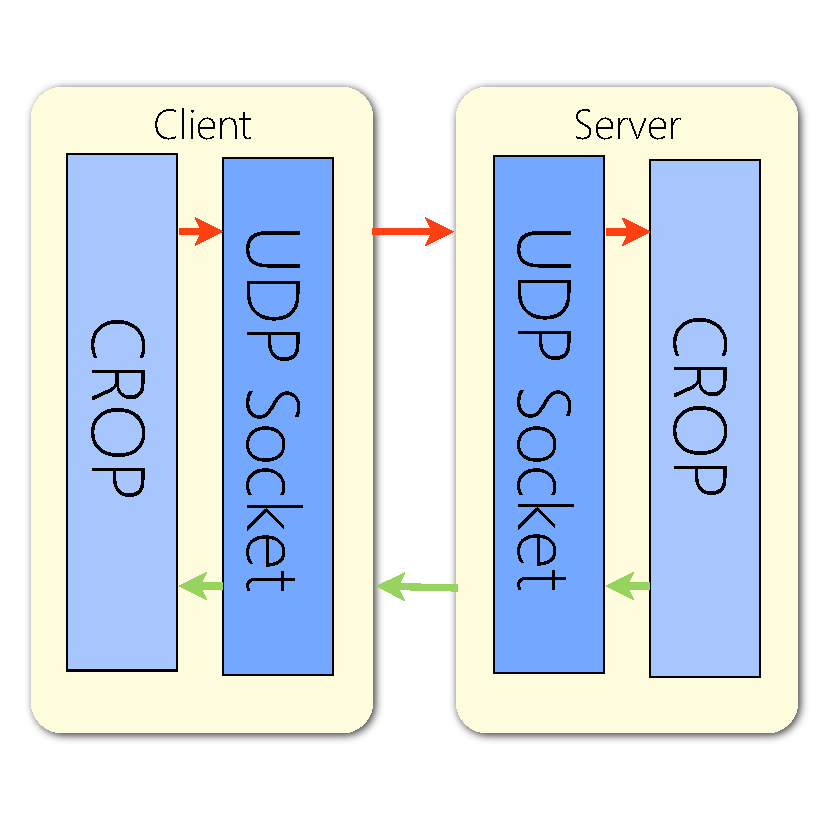
\includegraphics[scale=.5]{UDP_CROP.pdf}
\caption{Client/Server Kommunikation {\"u}ber UDP-Socket}
\label{fig:Socket-Kommunikation}
\end{figure}

Die Abbildung \ref{fig:Socket-Kommunikation} zeigt eine vereinfachte Darstellung
der Socket Kommunikation zwischen Client und Server mit aufsetzender Content
Relevance-Oriented Priorization bzw. aufsetzendem \gls{ROTP}. In Abbildung
\ref{fig:OSI} erfolgt eine Einordnung des \gls{CROP}/\gls{ROTP} in das OSI-Referenzmodell.

\begin{figure}[H]
\centering
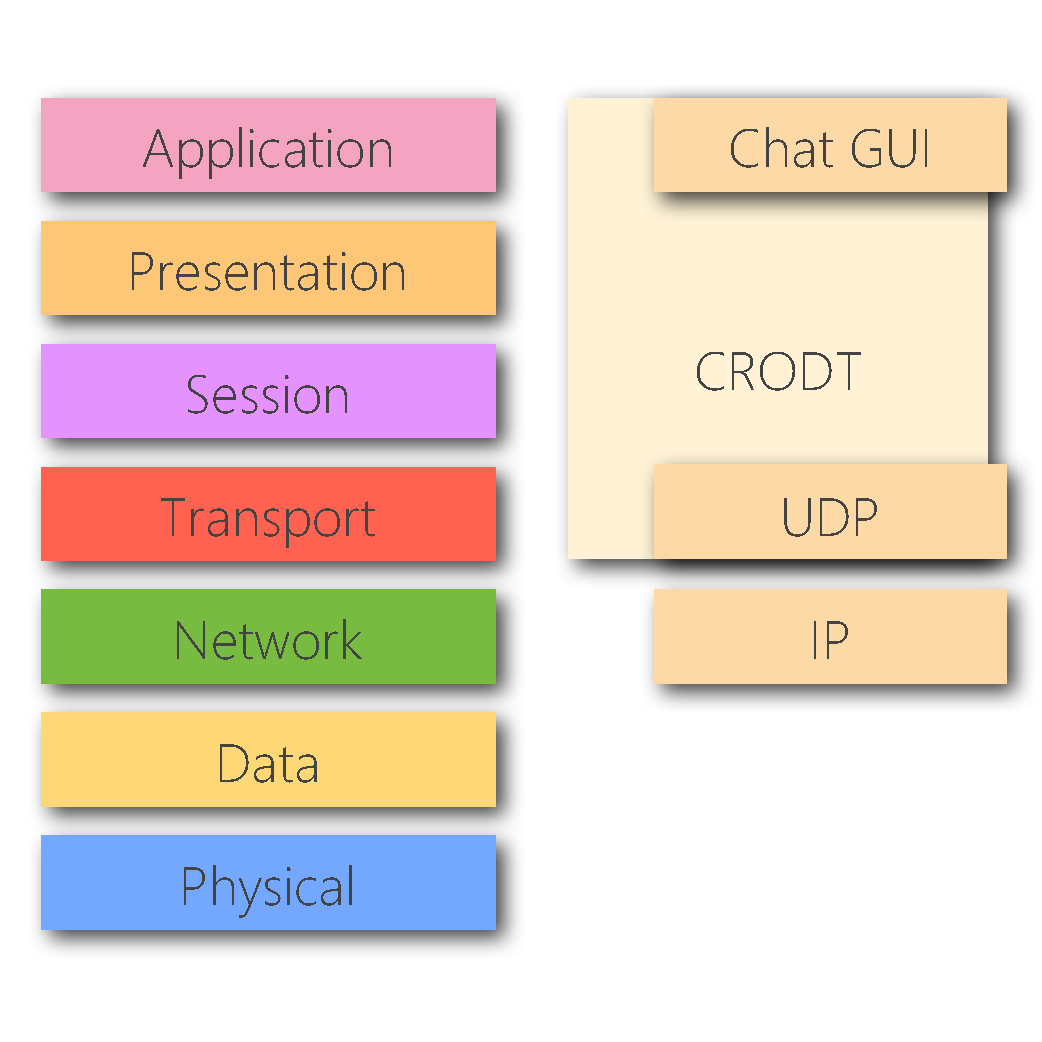
\includegraphics[scale=.38]{OSI.pdf}
\caption{{\"U}berblick des OSI-Schichtenmodells und der Zuordnung von CROP/ROTP}
\label{fig:OSI}
\end{figure}

\subsection{StoreManager}

W{\"a}hrend der Entwicklung des Moduls \Code{Sender} kristallisierte sich eine
weitere notwendige Eigenschaft der Software heraus. Diese beruht auf den
extremen Bedingungen die auf dem Mars herrschen. So kann jederzeit die
Möglichkeit bestehen, dass das Programm abstürzt oder die Stromzufuhr
unterbrochen ist. Auch unter diesen Bedingungen sollen die Daten noch vorhanden
sein, welche w{\"a}hrend des Progammablaufes erstellt und zum Versenden
gespeichert werden. Weil die Klasse \Code{SmartPrioritizedQueue}
die Daten im Arbeitsspeicher hinterlegt, w{\"a}ren diese bei einem Absturz verloren.
F{\"u}r das Abspeichern der Daten auf einem Speichermedium existieren
prinzipiell drei Methoden.

\begin{enumerate}
\item Jede erzeugte Variable wird direkt auf der Festplatte abgespeichert.
\item Ein Datenpaket (mehrere Variablen) wird an einer Stelle im Programm auf
einmal gespeichert.
\item Es werden Interrupts des Prozessors abgefangen, um Abst{\"u}rze zu erkennen,
infolgedessen werden alle wichtigen Daten gesichert.
\end{enumerate}

Die erste Methode hat den Vorteil, dass alle Daten sofort gesichert werden und
diese somit nicht verloren gehen k{\"o}nnen. Jedoch sind daf{\"u}r sehr viele
Festplattenzugriffe notwendig, wodurch die Laufzeit des Programms stark
beeintr{\"a}chtigt wird. Bei der dritten Methode sind die Festplattenzugriffe
minimal, jedoch k{\"o}nnen nur Software- und Hardwarefehler bei der
Programmabarbeitung abgefangen werden. Bei einem Stromausfall w{\"u}rden
trotzdem alle Daten verloren gehen. Deshalb wird Methode Zwei verwendet. Diese
stellt den besten Kompromiss aus Datensicherheit und Performance dar. \newline
F{\"u}r diese Aufgabe wurde ein Submodul entwickelt, welches die Datenbl{\"o}cke
auf der Festplatte hinterlegt und bei einem Absturz neu l{\"a}dt und damit die
\Code{SmartPrioritizedQueue} vorinitialisiert. Dadurch sind die Schnittstellen,
welche das Modul bereitstellen soll, schon indirekt vorgegeben. Diese sind eine
Methode, welche Datenbl{\"o}cke auf der Festplatte speichert, eine weitere, um
diese zu laden und eine Dritte, mit der bereits gespeicherte Datenbl{\"o}cke
gel{\"o}scht werden k{\"o}nnen.

\begin{figure}[H]
\centering
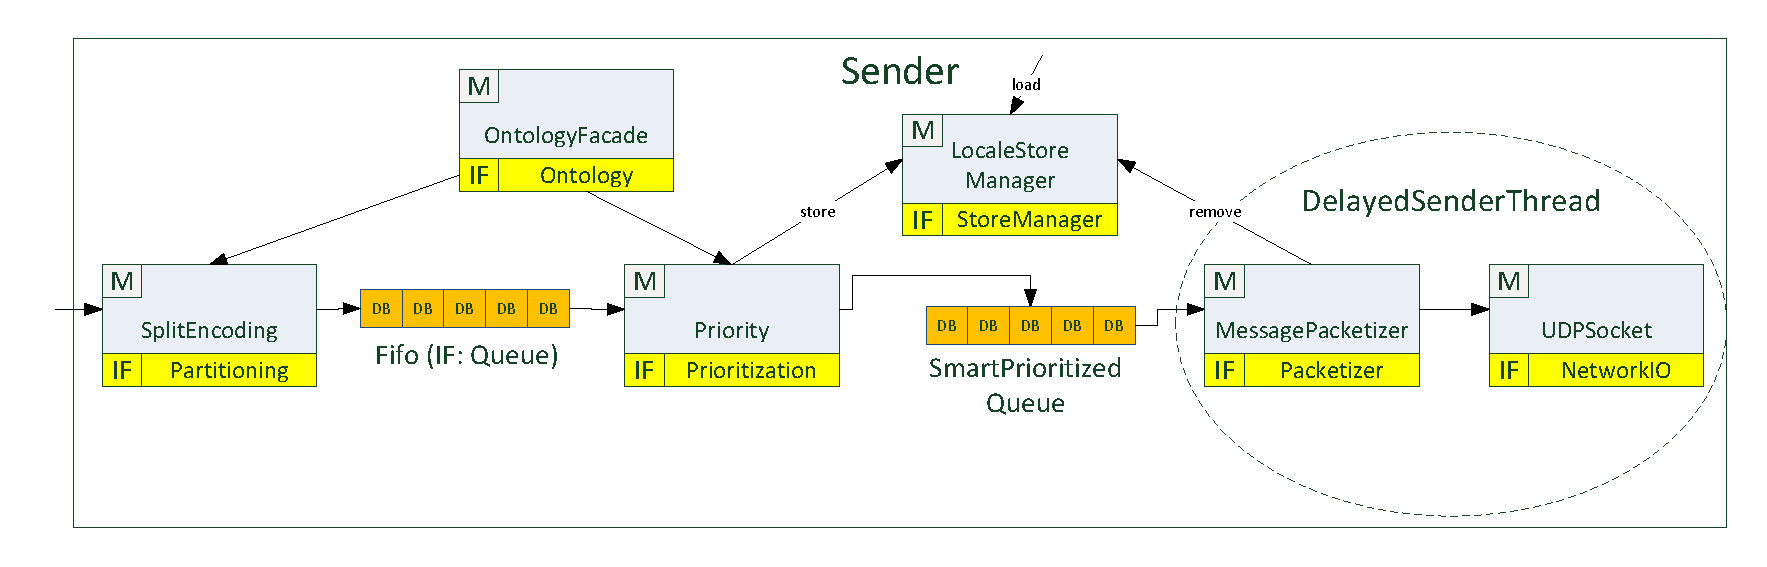
\includegraphics[scale=.49]{EinbettungStoreManager.pdf}
\caption{Integration des Submoduls \Code{StoreManager}}
\label{fig:EinbettungStoreManager}
\end{figure}

Die Einbettung des Submoduls \Code{StoreManager} in das Modul \Code{Sender} ist
in Abbildung \ref{fig:EinbettungStoreManager} veranschaulicht. Dazu wird der
\Code{StoreManager} parallel zur \Code{SmartPrioritizedQueue} integriert. Alle
Datenbl{\"o}cke, welche in die Queue gelangen, werden ebenfalls an die
Klasse \Code{StoreManager} {\"u}bergeben. Die von dem Submodul \Code{Packetizer}
gelesenen Datenbl{\"o}cke werden anschließend wieder gel{\"o}scht. Somit ist immer der
aktuelle Datenbestand der \Code{SmartPrioritizedQueue}
zus{\"a}tzlich auf der Festplatte gesichert. Beim Programmstart wird in der
Initialisierungsmethode des Topmoduls {\"u}berpr{\"u}ft, ob bereits alte Daten vorhanden
sind, welche anschlie{\ss}end geladen werden. \newline
F{\"u}r das Abspeichern der
Daten fehlt noch ein passendes Dateiformat, welches ein schnelles Speichern und
Lesen erm{\"o}glicht. Dazu wurden zwei M{\"o}glichkeiten gegen{\"u}bergestellt. Diese sind
in Tabelle \ref{tab:Speicherformate} aufgef{\"u}hrt.

\begin{longtable}{|lcc|}
\caption{Vergleich der Speicherformate} \\
\hline
\label{tab:Speicherformate}
\textbf{} & \textbf{XML-Datei} & \textbf{Bin{\"a}re Datei}\\
\hline
  Menschliche Lesbarkeit      &  + & - \\
  Dateigr{\"o}{\ss}e      &  0 & + \\
  Geschwindigkeit &  0 & + \\
  Portabilit{\"a}t    &  + & - \\
\hline
\caption*{ + Gut, 0 Medium, - Schlecht }
\end{longtable}

Der Tabelle \ref{tab:Speicherformate} ist zu entnehmen, dass \gls{XML} auf den
ersten Blick das bessere Format ist. Dennoch wurde eine bin{\"a}re Datei
verwendet, da die beiden entscheidenden Schwachstellen (die Portabilit{\"a}t und
die Lesbarkeit) f{\"u}r einen Menschen im konkreten Anwendungsfall keine
Bedeutung haben.
Weiterhin soll nur der Computer die Daten auf der Festplatte ablegen und
wieder lesen k{\"o}nnen. F{\"u}r das Versenden {\"u}ber das Internet oder
andere Medien besitzt die Portabilit{\"a}t zudem keinen gro{\ss}en Stellenwert.
Daf{\"u}r sind die beiden wichtigsten Eigenschaften, die Dateigr{\"o}{\ss}e und die
Geschwindigkeit, beim gew{\"a}hlten Format im Vergleich besser.
\newline
In der Datei werden die folgenden Daten aus dem Datenblock in der
aufgef{\"u}hrten Reihenfolge gespeichert:

\begin{itemize}
\item Datenblockheader 
\item Priorit{\"a}t
\item Zeitstempel
\item Content als ByteArray
\end{itemize}

Für den Datenblockheader ist eine Kompression möglich und dadurch kann der
Speicherplatzbedarf der Variablen unterschiedlich sein. Deshalb wird f{\"u}r
diese festgelegt, dass die h{\"o}chste auftretende Bitzahl f{\"u}r jeden Wert zur
n{\"a}chsten Zweierpotenz und ganzem Byte aufgerundet wird.
Dadurch wird das Laden und Speichern stark vereinfacht. Der dabei auftretende
zus{\"a}tzliche Speicherplatzbedarf kann vernachl{\"a}ssigt werden.
\newline 
F{\"u}r die Ordnerstruktur wurde eine m{\"o}glichst flache Hierarchie genutzt,
welche in der obersten Stufe den Ordner \Code{Backup} beinhaltet. Darin befinden sich
weitere Ordner, welche als Namen die Nummer des Datentypes beinhalten. In diesem
liegen die bin{\"a}ren Dateien, deren Namen aus der Nummer der \gls{DOID} und
der Sequenznummer bestehen.
Diese sind durch einen Unterstrich voneinander getrennt. Die drei Parameter
werden von der Methode remove zum L{\"o}schen einer Datei {\"u}bergeben, um diese
eindeutig zu identifizieren.

\section{Modulaufbau Empf{\"a}nger}

Auf der Empf{\"a}ngerseite sollen die ankommenden Nachrichten empfangen und geparst
werden, um an die darin enthaltenen Informationen zu gelangen. Das Empfangen
durch das Submodul \Code{UDPSocket} ist blockend. Deswegen wird der Vorgang
nebenl{\"a}ufig ausgef{\"u}hrt, damit der Programmablauf nicht behindert wird.
Anschließend wird die Nachricht geparst und nach dem Beenden des Vorganges ein Callback
ausgel{\"o}st. Bei einem Callback wird ein Zeiger auf die Speicheradresse der
Funktion in der Klasse gespeichert. Durch Aufruf der Funktion ist es
m{\"o}glich, den sequentiellen Programmablauf an einer anderen Stelle
weiterlaufen zu lassen. Nach Abarbeitung dieser kehrt der Ablauf zur
urspr{\"u}nglichen Position zur{\"u}ck. Diese Funktion kann mittels einer
Methode registriert werden, in der die geparsten Daten weiter verarbeitet werden
k{\"o}nnen.
Die Callbackfunktion k{\"o}nnte beispielsweise die Visualisierung und das
Zwischenspeichern der unvollständigen Daten {\"u}bernehmen. \newline 
In Abbildung \ref{fig:BlockdiagrammEmpfaenger} wird eine schematische
Darstellung des Moduls angezeigt. Eine weitere detaillierte Übersicht der Klassen
und deren Interaktion untereinander ist im Anhang
\ref{fig:KlassendiagrammParser} in Form eines Klassendiagramms 
abgebildet.
Die Implementierung wird im Folgenden n{\"a}her erl{\"a}utert.

\begin{figure}[H]
\centering
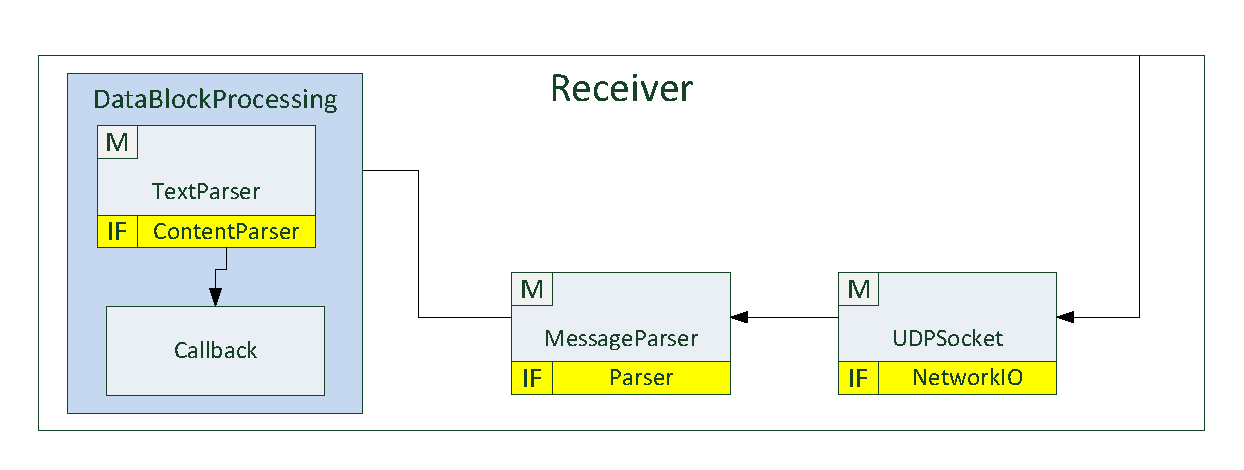
\includegraphics[scale=.6]{BlockdiagrammEmpfaenger.pdf}
\caption{{\"U}bersicht des Empf{\"a}ngers}
\label{fig:BlockdiagrammEmpfaenger}
\end{figure}

\subsection{Parser}

Der Parser basiert auf dem in Kapitel \ref{sec:ProtokolDesign}
vorgestellten Protokoll-Design.
Anhand dieser Daten wird die empfangene Nachricht Bit f{\"u}r Bit analysiert
und die Informationen herausgezogen. 
Die Klasse \Code{UDPSocket} empf{\"a}ngt neue Daten und gibt diese an
die Klasse \Code{MessageParser} weiter. Dieser parst den Nachrichtenheader.
Dessen Algorithmus ist in Abbildung \ref{fig:AlgorithmusMessageParser}
dargestellt.
Anschlie{\ss}end werden die Datenblockheader geparst. Der Content wird von der
Klasse \Code{DataBlockProcessing} verarbeitet.

\begin{figure}[H]
\centering
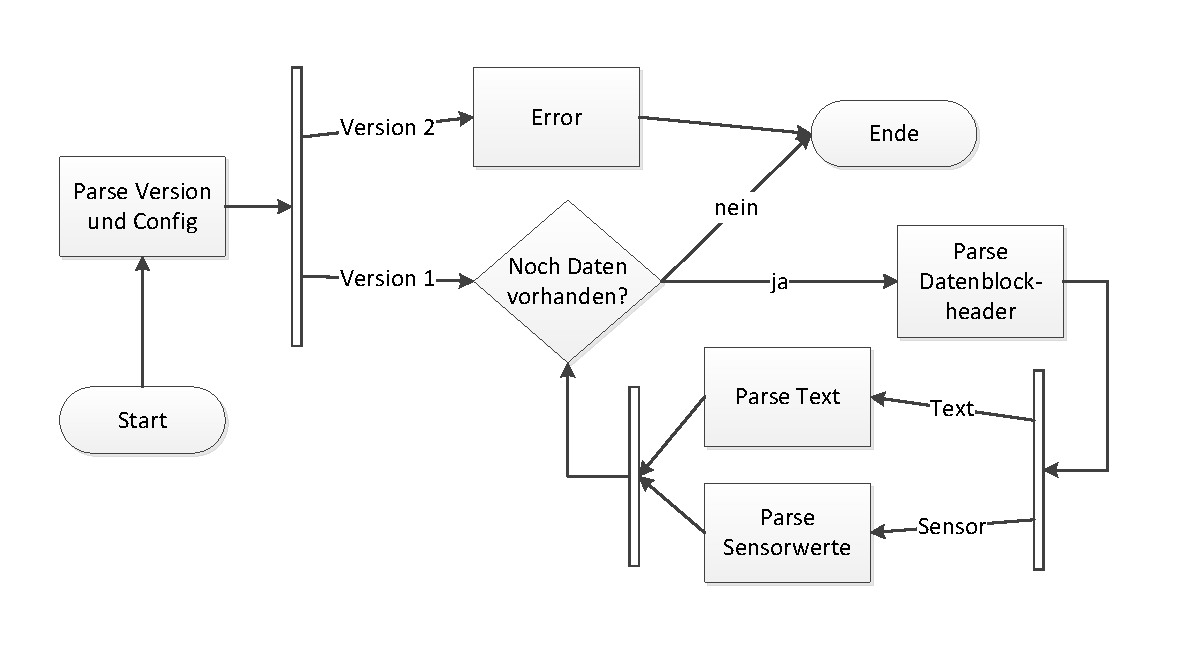
\includegraphics[scale=.6]{AlgorithmusMessageParser.pdf}
\caption{Algorithmus zum Parsen der Nachricht}
\label{fig:AlgorithmusMessageParser}
\end{figure}

Daf{\"u}r wird ein Softwarekonzept namens Policy-Based-Template-Meta Programmierung
verwendet \cite{Alexandrescu:2001:MCD:377789}, damit die
unterschiedlichen Datentypen der Datenbl{\"o}cke nach dem Parsen wieder in einem
typsicheren Format vorliegen und einfacher verwendet werden k{\"o}nnen.
Der Templateklasse werden die folgenden vier Klassen als Templateparameter
Klasse {\"u}bergeben:

\begin{itemize}
\item T - Datentyp des R{\"u}ckgabewertes des Parsers
\item Parser - Klasse zum Parsen des Datentypes
\item C - Datentyp, der als Callback zur{\"u}ckgegeben wird
\end{itemize}

Der Parameter \Code{Parser} erbt zus{\"a}tzlich von einer
Schnittstelle gleichen Namens. Die Klasse \Code{DataBlockProcessing} erbt
wiederum von dem Parameter \Code{Parser}.
Dadurch besteht die M{\"o}glichkeit, in der Klasse auf Funktionen und
Membervariablen zugreifen zu k{\"o}nnen.
Durch dieses Vorgehen kann das Verhalten der Klasse einfach durch die
Templateparameter ver{\"a}ndert werden. Weil der Grundalgorithmus des Parsers
f{\"u}r die Datenbl{\"o}cke bei jedem Datentyp identisch ist und lediglich die
Art und Weise ver{\"a}ndert werden muss, wie die Daten geparst werden,
ist dieser Weg der optimale. Durch das Konzept wurden
Redundanzen im Quellcode vermieden und weitere Datentypen lassen sich
sehr einfach hinzuf{\"u}gen ohne bestehenden Quellcode zu ver{\"a}ndern. Dadurch konnten
die Grundprinzipien der objektorientierten Programmierung eingehalten werden \cite{herold2001go}.
Der eben angesprochene Grundalgorithmus, welcher f{\"u}r jeden Datentyp
durchlaufen wird, ist in Listing \ref{lst:PseudocodeDBParser} dargestellt.

\lstdefinelanguage{pseudo}{
morekeywords={if, else, for, in, remove, from, case, do, forever, to, false,
function, then, end, true, while}, sensitive=true,%
morecomment=[l]\#,%
morestring=[b]',%
}
\lstset{language=pseudo}
\lstset{commentstyle=\textit}
\lstset{literate=
 {<=} {$\le$}{2} {!=} {$\neq$}{2} {=} {$\leftarrow$}{2} {==} {=}{2} {&&}
{$\cap$}{2} {||} {$\cup$}{2} } \lstinputlisting[label=lst:PseudocodeDBParser,caption=Pseudocode
des Datenblock Parsers]
{Listings/PseudocodeDBParser.txt}

	\section{ChatGui}
	Dieser Abschnitt unserer Arbeit befasst sich mit dem entwickelten
GUI. Benutzeroberfl{\"a}che zu Programmieren, durch welche eine Chat
Kommunikation via CRODT Protokoll vorgenommen werden kann. Hierbei galt es
Grundlegende Betrachtungen bez{\"u}glich des Interfaces anzustellen. Auf Basis
der Design Regeln nach Nielsen wurde der erste Prototyp entwickelt. Das GUI
besteht aus dem Empfangsfenster (Abb 1. oben links) dem Eingabenfenster (Abb 1.
unten links) sowie der Priorit{\"a}tenliste (Abb 1. oben rechts) und den
Bedienelementen (Abb 1. unten rechts). Die Implementierung erfolgte dabei in
C++ durch Nutzung der Qt-Bibliothek. Da f{\"u}r unsere Arbeit aufgrund der
begrenzten zeit keine M{\"o}glichkeit f{\"u}r eine Nutzerzentrierte GUI
Entwicklung war, wurde der bereits erw{\"a}hnte Nutzerunabh{\"a}ngige Entwurf
nach Jakob Nielsen gew{\"a}hlt. Dieser Entwurf sieht eine Planung nach zehn
Regeln vor.

Regeln des GUI Designentwurfs nach Jakob Nielsen:

   \begin{enumerate}[I]
     \item Nutzung Einfacher und nat{\"u}rlicher Dialoge
     \item Verwendung der Nutzersprache
     \item Minimierung der Ged{\"a}chtnislast des Nutzers
     \item Nutzung konsistenter Formulierungen
     \item Dem Nutzer stets Feedback geben
     \item Klar markierte Navigationsm{\"o}glichkeiten anbieten
     \item Dem Nutzer Shortcuts anbieten
     \item Lieferung genauer Fehlermeldungen
     \item Vermeidung vermeidbarer Fehler
     \item Bereitstellen einer Hilfe und Dokumentation
   \end{enumerate}

Je nach Komplexit{\"a}t des vorliegenden Projekts gilt es einzelne Punkte
hierbei eventuell schwerer zu gewichten als andere. So steigt z.B. bei
zunehmender Komplexit{\"a}t des GUI die Wichtigkeit einer ausf{\"u}hrlichen
Hilfe und Dokumentation. Da die Komplexit{\"a}t des GUI im Szenario der
Projektarbeit {\"u}berschaubar ist, verzichten wir auf eine Hilfe Funktion und
ersetzen diese durch eine Ausf{\"u}hrliche Dokumentation.

\begin{figure}[H]
\centering
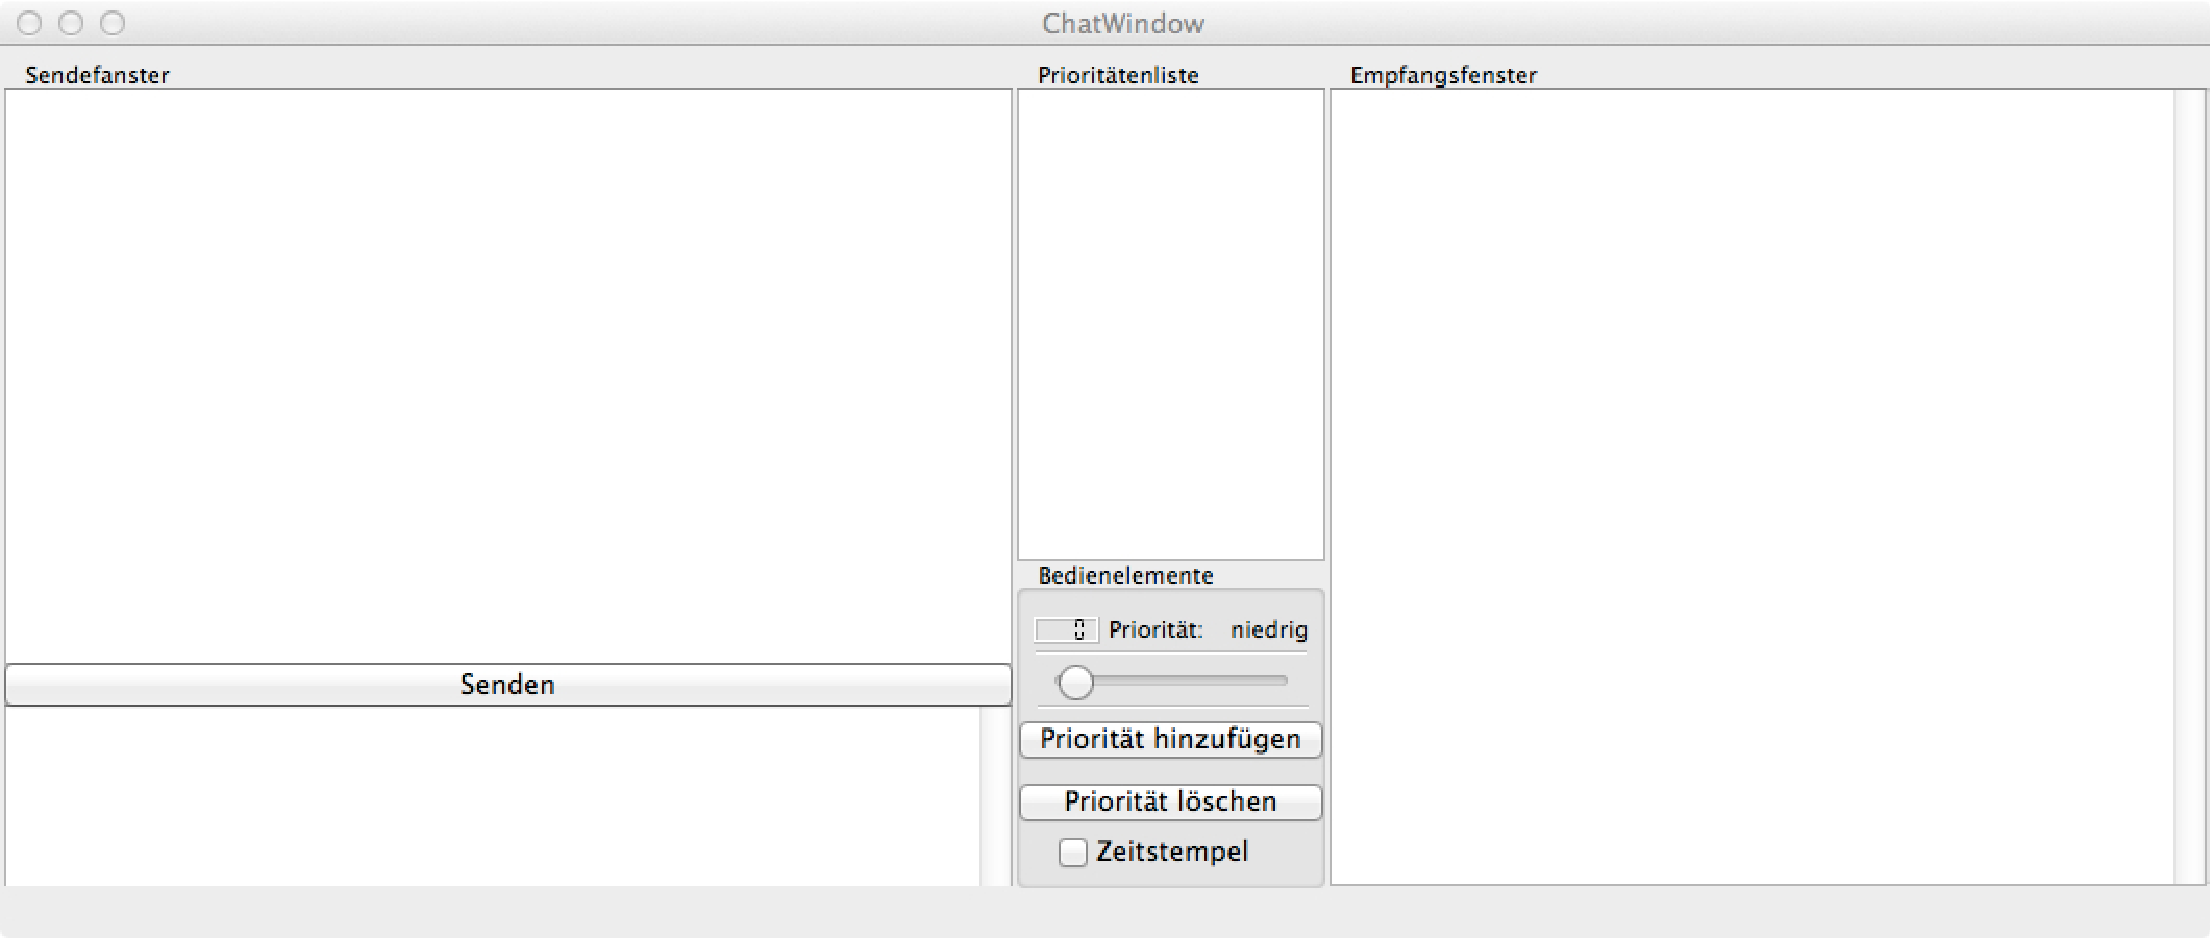
\includegraphics[scale=.38]{GUI_1.pdf}
\caption{Grafisches User Interface (MarsChat)}
\label{fig:Grafisches User Interface}
\end{figure}

\begin{figure}[H]
\centering
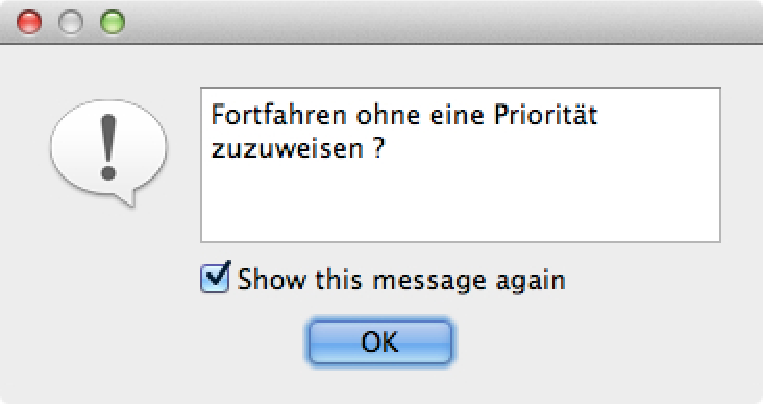
\includegraphics[width=8cm]{Msg_1.pdf}
\caption{Beispiel einer optionalen Mitteilung}
\label{fig:Message1}
\end{figure}

\begin{figure}[H]
\centering
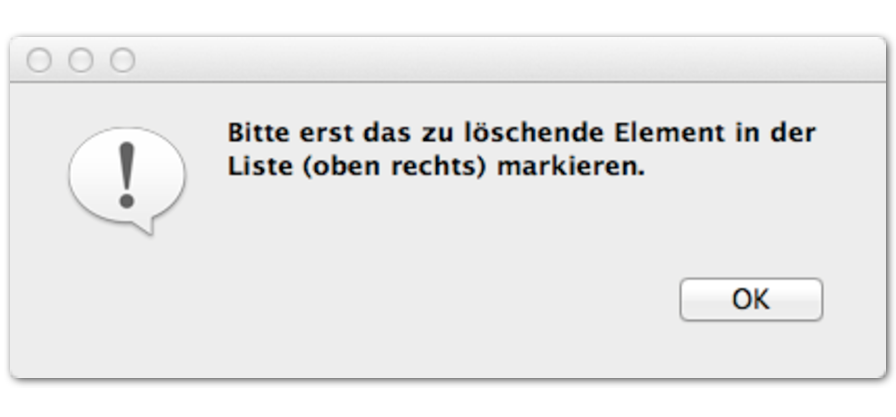
\includegraphics[width=8cm]{Msg_2.pdf}
\caption{Beispiel einer Information}
\label{fig:Message2}
\end{figure}

\begin{figure}[H]
\centering
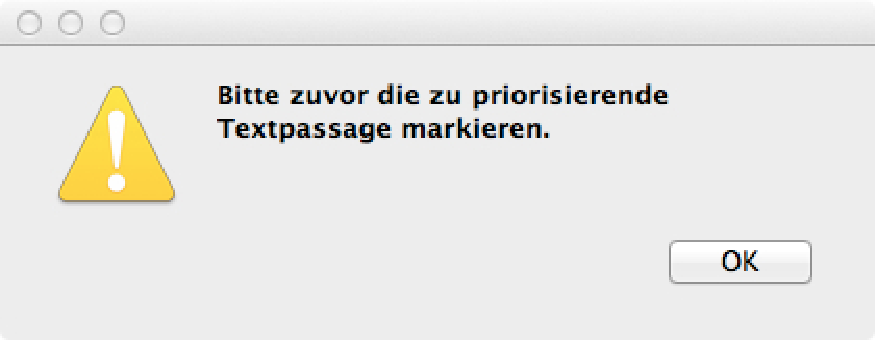
\includegraphics[width=8cm]{Msg_3.pdf}
\caption{Beispiel einer Warnung}
\label{fig:Message3}
\end{figure}


\chapter{Protokoll-Analyse}
	\label{cap:protokollAnalyse}
Zur fundierten Aussage über die Funktionsfähigkeit und -tragweite des CROP wurde
dieses hinsichtlich unterschiedlicher Aspekte untersucht. Dazu gehört neben der
Laufzeit und Paketgröße auch der Overhead. Unter verschiedenen Einstellungen
wurden mehrere Messreihen aufgenommen, welche im Folgenden näher vorgestellt und
diskutiert werden.

	\section{Overhead}
		Wie bereits im Kapitel \ref{sec:ProtokolDesign} erläutert, existiert neben den
eigentlichen Daten der Header. Die zusätzliche Größe, um die sich die
zu versendende Nachricht dadurch erhöht, heißt Overhead. Die Berechnung und
Bedeutung dessen wird im Folgenden beschrieben.

Ausgehend vom Aufbau einer Nachricht (siehe Abbildung
\ref{fig:uebersichtdatenaufschluesselung}) sind bei der Berechnung des Overhead
zwei Header zu betrachten. Einerseits ist dies der allgemeine Header der
Nachricht und zum Anderen trägt jeder einzelne Datenblock
mit einem eigenen Header zum Overhead bei. Dies kann durch die Formel
\ref{eq:overhead} ausgedrückt werden.

\begin{equation}
	Overhead = Overhead_{Nachricht} + n * Overhead_{Datenblock}
	\label{eq:overhead}
\end{equation}

Dabei variiert die Größe des Nachrichtenheaders je nach gewähltem
Übertragungsprotokoll (Formel \ref{eq:overheadMessage}). In dem Protokoll,
welches in dieser Arbeit vorgestellt wird, ist dies das IPv6. Das IPv6
reserviert $32$ Byte im Header. Damit ergibt sich für diesen speziellen Fall $37$ Byte für
den Nachrichtenheader. Ein Datenblockheader besteht immer konstant aus $9$ Byte.
Die angedeutete Kompressionseinstellung findet in dieser Arbeit noch
keine Berücksichtigung.

\begin{equation}
	Overhead_{Nachricht} = 5 Byte + Address_{Source} + Address_{Destination}
	\label{eq:overheadMessage}
\end{equation}

Aus der Formel \ref{eq:overhead} ist zu erkennen, dass der Overhead
stetig mit der Anzahl an gleichzeitig zu verschickenden Datenblöcken ($n$)
steigt. Einzig der Nachrichtenoverhead hat für große $n$ nur noch eine
geringe Auswirkung. Somit ist ein Versenden einer Nachricht mit vielen Daten
gleichzeitig sinnvoller, um überflüssigen Overhead zu vermeiden. Dieser
Effekt wird mit Formel \ref{eq:overheadRatio} noch einmal verdeutlicht. Diese
gibt das Verhältnis der Größe von Overhead zur gesamten Nachricht an und
ermöglicht eine prozentuale Aussage.

\begin{eqnarray} 
	overhead_{ratio} & = & \frac{Overhead}{Nachricht_{gesamt}}\\
	overhead_{ratio} & = & \frac{Overhead_{Nachricht} + n *
	Overhead_{Datenblock}}{Overhead_{Nachricht} + n * (Overhead_{Datenblock} + Content)}\\
	overhead_{ratio} & = & \frac{Overhead}{Overhead + n * Content}
	\label{eq:overheadRatio}
\end{eqnarray}
	\section{Messreihen}
		\label{subCap:Messreihen}


\textbf{Testumgebung}

Die Messungen wurden mit einem Notebook aufgenommen, welches
folgende Hardwarekonfigurationen besitzt.

\textit{
	LENOVO Thinkpad t410 Modell 2522-w29 \newline
	\textbf{Prozessor}: Intel Core i5 520M (2 Kerne mit Hyperthreading $\stackrel{\wedge}=$ 4 Threads)\\
	\textbf{Arbeitsspeicher}: 4 GB DDR3	
	}

Da eine ähnliche Hardware bei einer Verwendung des Protokolls auf dem Mars
weniger zu erwarten ist, sind die Größenordnungen der nachfolgenden Ergebnisse
nur ein Richtwert. Für die folgenden Betrachtungen sind die Beziehungen und
Entwicklungen der einzelnen Werte zueinander wichtig, welche mit schwächerer
Hardware nahezu identisch sind. Zum Vergleich der weniger performanten Curiosity
Computer sei auf das Kapitel \ref{cap:standDerTechnik} verwiesen. 
\\

\textbf{Methodik}


	\section{Ergebnisse und Diskussion}
		Die Abbildung \ref{fig:diagrammInitial_worp} zeigt grafisch die Ergebnisse der
Messreihen für den initialen Durchlauf ohne relevante Bereiche. Dabei ist die
Laufzeit in $\mu s$ über die Textgröße in Byte logarithmisch aufgetragen. Für
relativ kleine Textgrößen hat die Geschwindigkeitsoptimierung noch keinen großen
Einfluss. Erst bei einer Größe von $5.000.000$ ($99\ \mu s$) oder
$10.000.000$ ($122\ \mu s$) Byte ist der erwartete Geschwindigkeitsprofit zu
verzeichnen.

\begin{figure}[H]
	\centering
	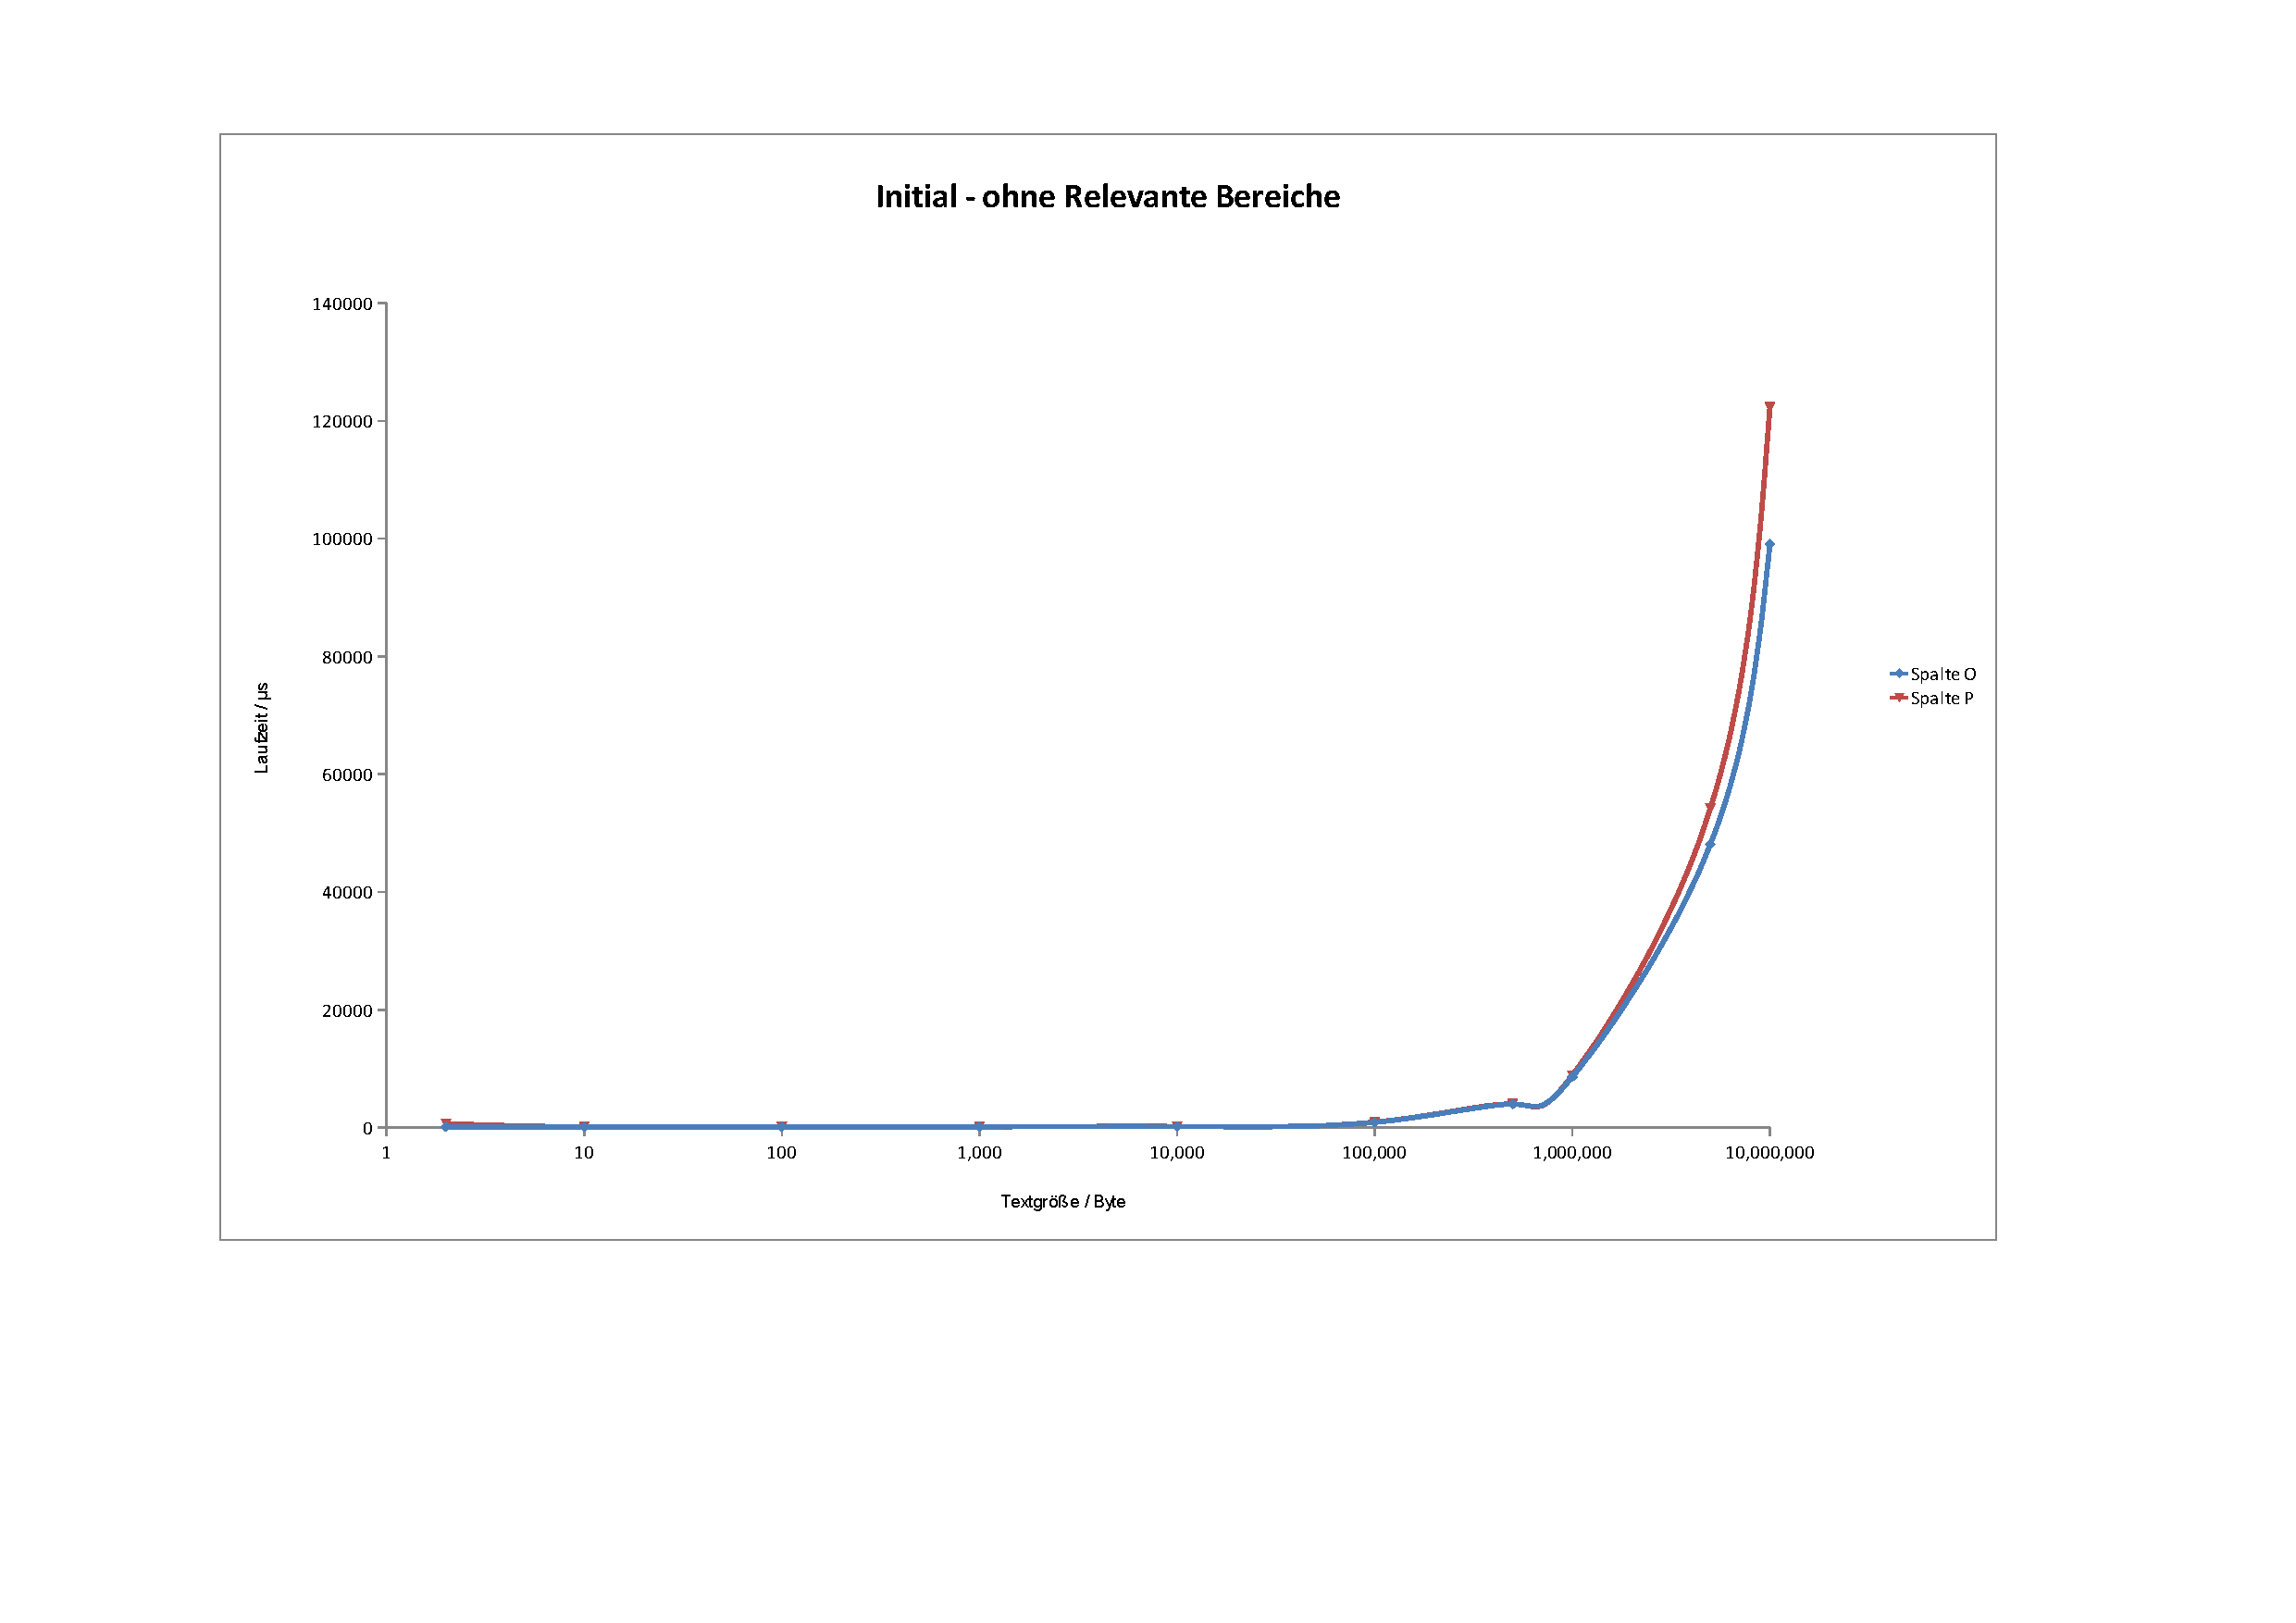
\includegraphics[scale=.45]{DiagrammInitial_worp.pdf}
	\label{fig:diagrammInitial_worp}
	\caption{Messung-Initial ohne relevante Bereiche}
\end{figure}

Der Nachteil gegenüber der Quellcodegrößenoptimierung liegt darin, dass
mehr Speicherplatz in Anspruch genommen wird, wodurch der
Geschwindigkeitsvorteil erreicht werden kann.
Die Wahl der jeweiligen Optimierungsmöglichkeit ist situationsabhängig. Auf dem
Mars stehen weniger Speicherressourcen zur Verfügung, wodurch eine
Geschwindigkeitsoptimierung weniger sinnvoll erscheint. Die gleichen
Betrachtungen ergeben sich für alle anderen Messreihen (Abbildung im Anhang
\ref{sec:Diagramme}). 

\begin{figure}[H]
	\centering
	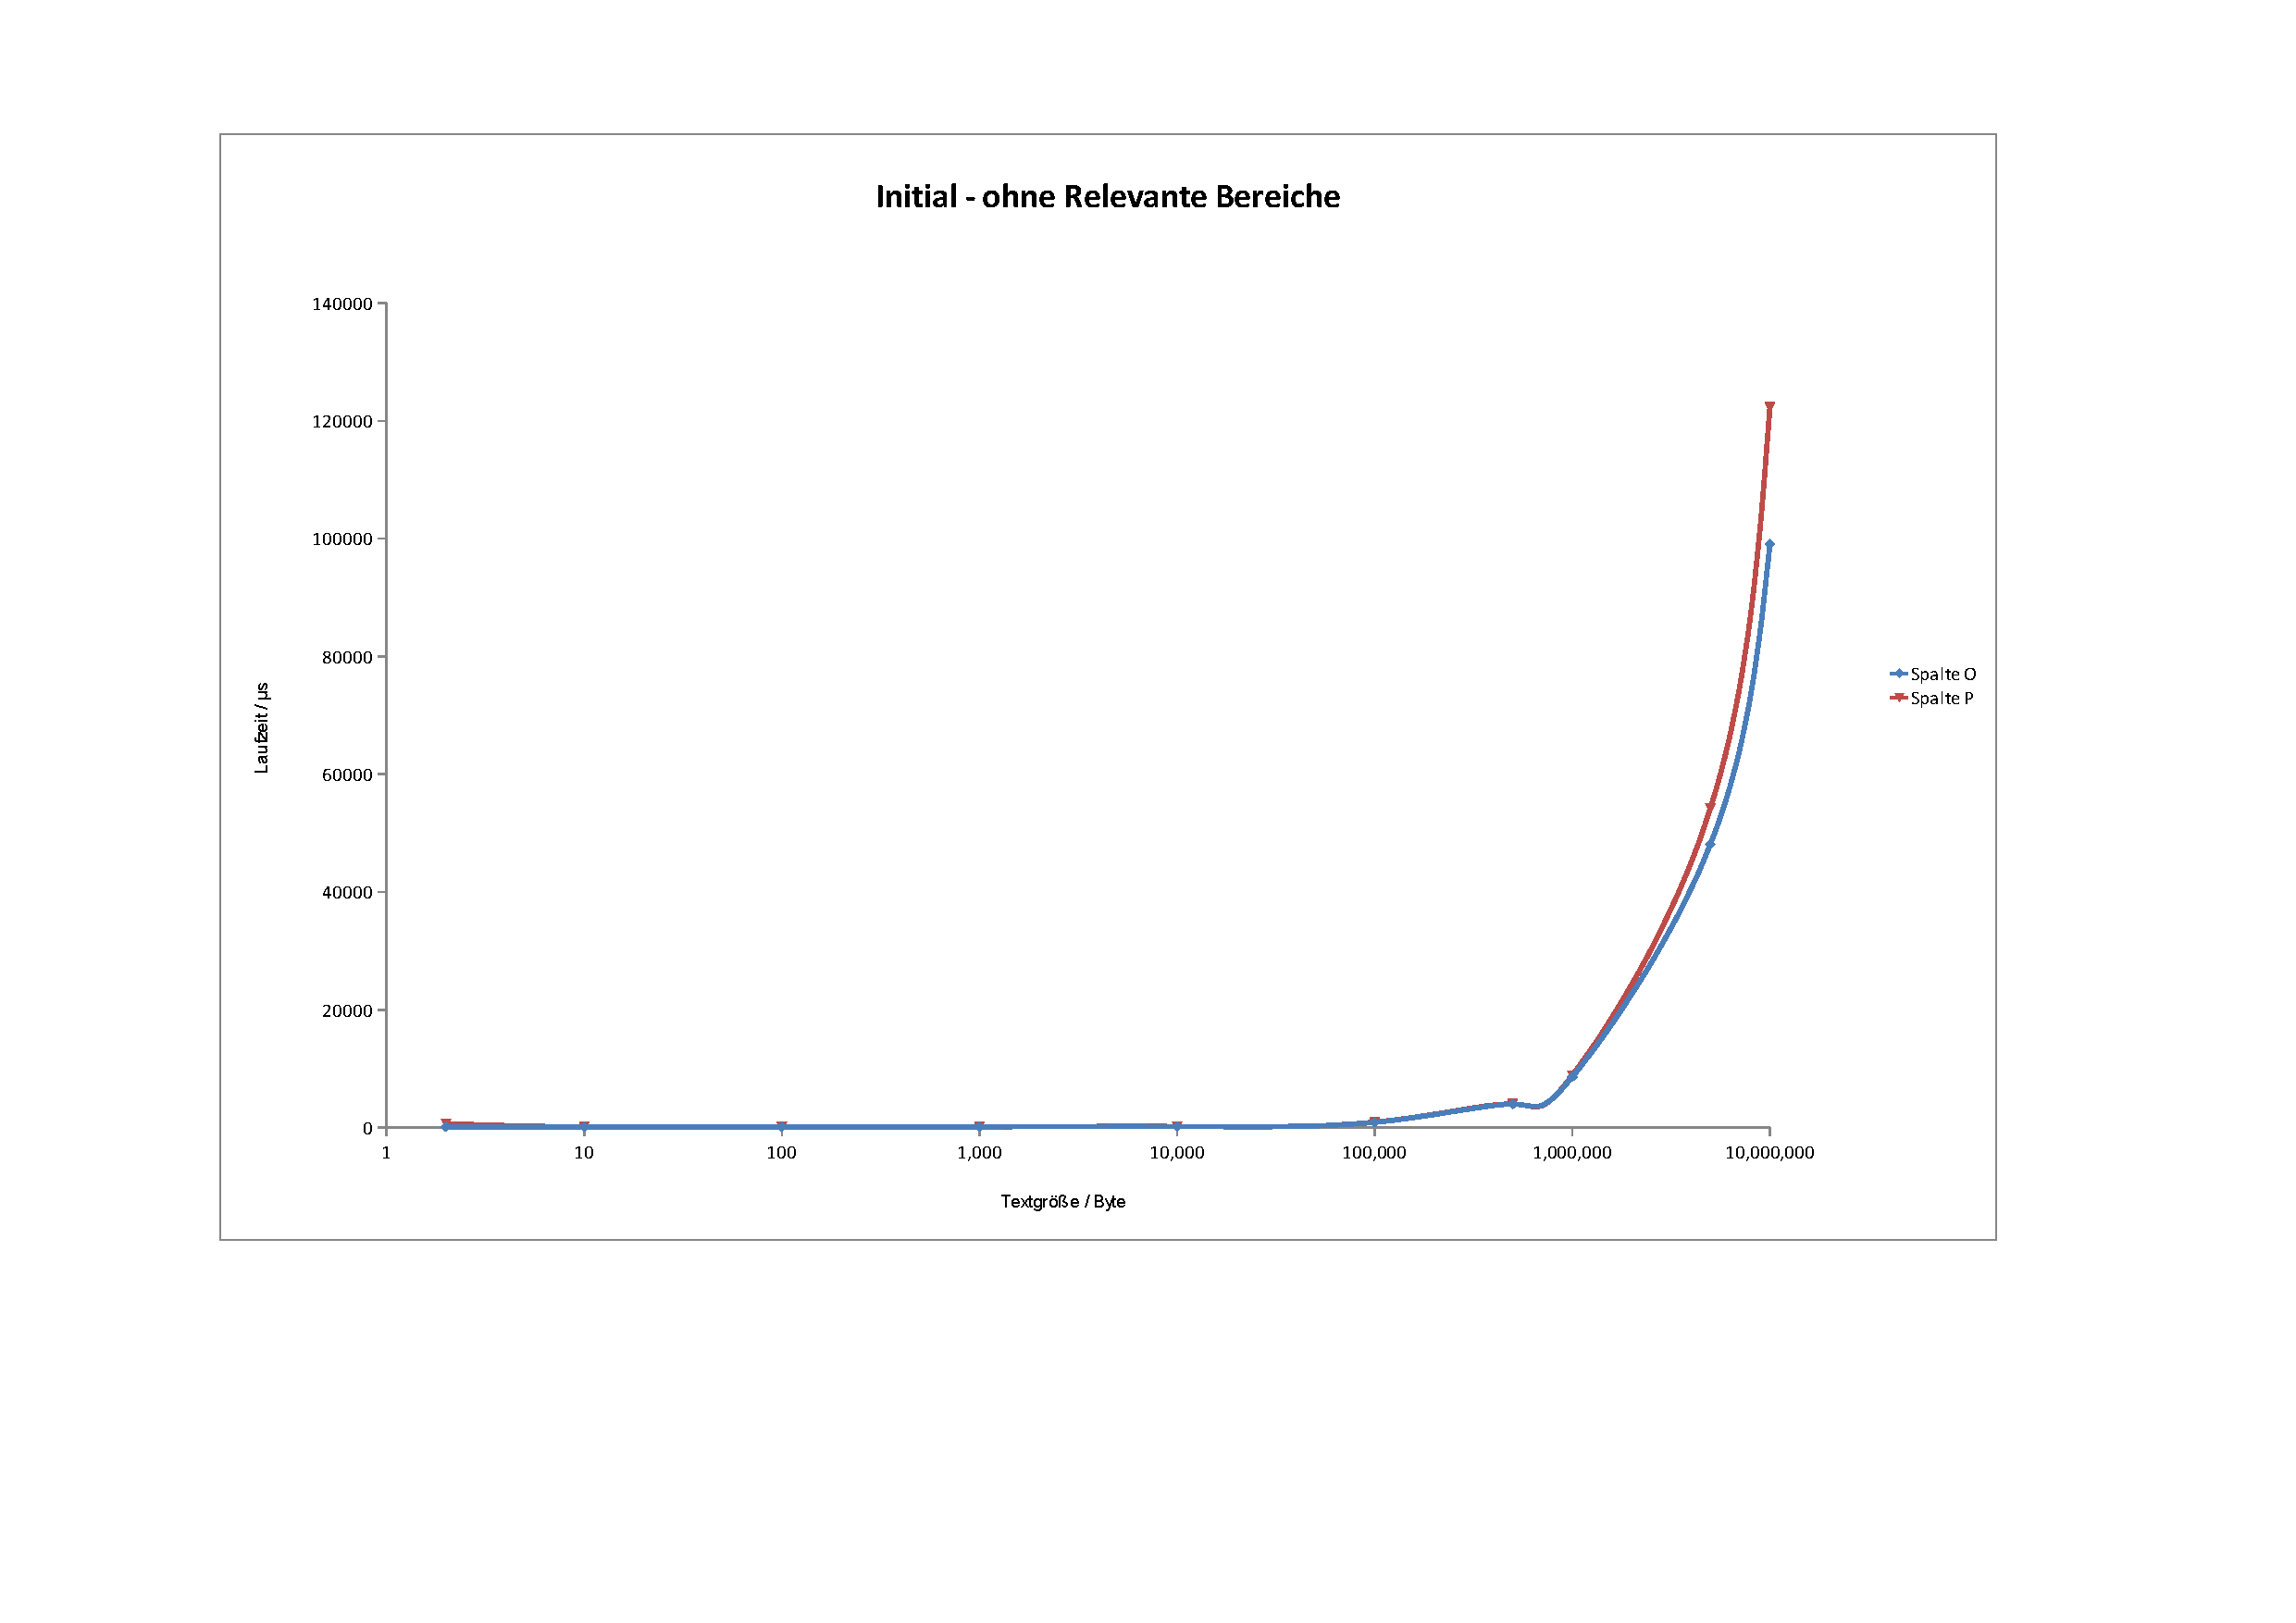
\includegraphics[scale=.45]{DiagrammInitial_worp.pdf}
	\label{fig:diagrammInitial_wrp}
	\caption{Messung-Initial ohne relevante Bereiche}
\end{figure}

In Abbildung \ref{fig:diagrammInitial_wrp} ist die Laufzeit bezüglich
verschiedener Anzahlen relevanter Bereiche dargestellt. Die Textgröße bleibt
dabei stetig bei $5.000.000$ Byte. Damit ist ein Vergleich der Werte mit den
durchschnittlichen Werten der gleichen Textgröße aus Abbildung
\ref{fig:diagrammInitial_worp} möglich. Für nur wenige relevante Bereiche
unterscheiden sich die Werte marginal. Steigt die Anzahl, nimmt die Laufzeit
jedoch exponentiell zu (siehe Abbildung \ref{fig:diagrammInitial}) und bewegt
sich dann im Millisekunden-Bereich. Dies bedeutet, dass die Implementierung noch
nicht für die Verwendung von einer sehr großen Anzahl an relevanten Bereichen
optimiert wurde. Im Kapitel \ref{sec:Anwendungsszenarien} wurden bereits
mögliche Anwendungsszenarien betrachtet, welche ebenso mit wenigen relevanten
Bereichen auskommen. Dadurch ist eine Optimierung an dieser Stelle vorerst
nebensächlich.

\begin{figure}[H]
	\centering
	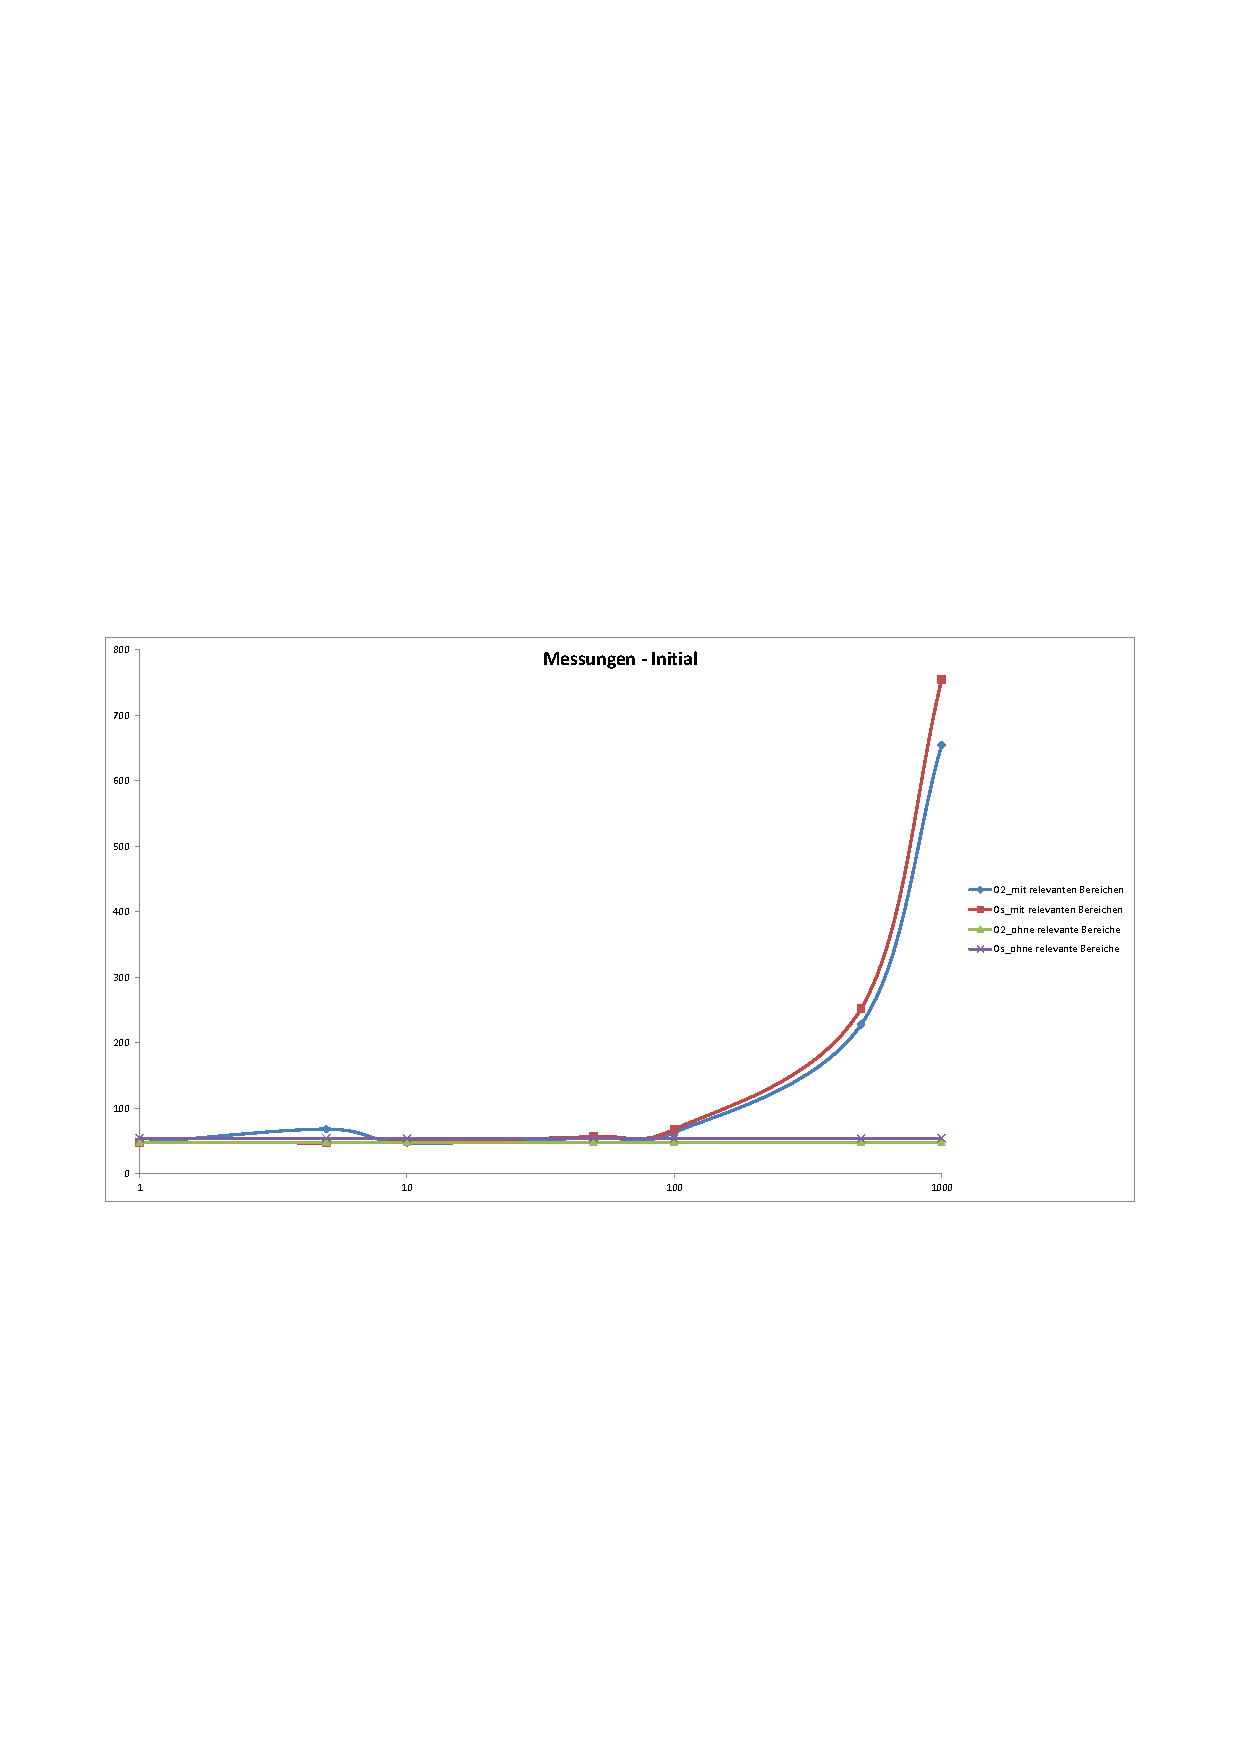
\includegraphics[width=\textwidth]{DiagrammInitial.pdf}
	\label{fig:diagrammInitial}
	\caption{Messung-Initial}
\end{figure}

Bei der letzten Messung werden nacheinander unterschiedliche
Datengrößen und zusätzlich Daten mit unterschiedlicher Anzahl an relevanten
Bereichen betrachtet. Dabei wird das Modul nicht neu erstellt. Hierbei ist zu
erkennen, dass die Verarbeitungsdauer ansteigt, je mehr Daten schon bearbeitet
wurden. Eine genauere Analyse zeigt, dass die priorisierende \gls{FIFO} der
Flaschenhals ist. Bei diesem Testdurchlauf wurden insgesamt $41.400$ Datenblöcke
aus $548$ MB verarbeitet.
Dabei lagen alle Datenblöcke gleichzeitig in der \gls{FIFO}, wodurch das Einsortieren neuer
Blöcke sehr viel Rechenleistung in Anspruch nimmt. Gleichzeitig werden diese
Daten im Arbeitsspeicher und auf der Festplatte gespeichert. Hierbei gilt zu
untersuchen, ob diese Form der Datensicherung bei einem Rover auf dem
Mars praktikabel ist, da dieser über sehr begrenzte Speicherressourcen verfügt.
Alternativ müssen neue Methoden gefunden werden, den Speicherverbrauch
einzuschränken. So besteht die Möglichkeit, die Daten nur auf der Festplatte
zu speichern und in der \gls{FIFO} die Indizes zu diesen zu hinterlegen,
wodurch der Speicherverbrauch im Arbeitsspeicher stark reduziert werden kann.
Allerdings ist diese Methode bei sehr vielen Daten nicht optimal, welche sich
bei sehr langen Zeiträumen, in denen nicht gesendet werden kann, ansammeln.
Eine bessere Möglichkeit wäre, anhand einer \gls{TTL} (siehe Kapitel
\ref{sec:Vorueberlegung}) unrelevante Daten nur sehr kurzfristig vorzuhalten,
damit mehr Raum für Daten von hoher Relevanz ist.


\chapter{Zusammenfassung und Ausblick}
	Für die interplanetare Kommunikation stehen besondere Aspekte, wie Latenz,
Bandbreite oder der lokale Speicher, im Vordergrund. Dazu ist ein besonderes
Kommunikationsprotokoll notwendig. Für dieses Protokoll \todo{LINK} existierte
bereits ein Konzept, welches im Rahmen dieser Arbeit verfeinert, implementiert
und bewertet werden sollte.

Dabei wird in Kapitel \ref{cap:standDerTechnik} und \ref{cap:grundlagen} ein
erster Überblick über den momentanen Stand der Technik, sowie Grundlagen zur
Einordnung der Thematik gegeben.

Die konzeptionelle Darstellung des Protokolls erfolgt in Kapitel
\ref{cap:konzept}. Dazu gehören neben möglichen Implementierungen und
Vorüberlegungen auch die eigentliche theoretische Umsetzung sowie Szenarien,
welche den Ablauf des Protokolls beispielhaft vorstellen. Der eigentliche
softwaretechnische Aufbau und die Implementierung wurden in Kapitel
\ref{cap:implementierung} detailliert beschrieben. Abschließend wurde das
Protokoll hinsichtlich Overhead, Laufzeit und Speicherbedarf analysiert und
ausgewertet (Kapitel \ref{cap:protokollAnalyse}).

Das in dieser Arbeit umgesetzte Protokoll bietet eine solide
Grundlage zur Relevanz-Orientierten Kommunikation. Jedoch besteht noch Raum
für Erweiterungen und Optimierungen.

Zum Einen wäre eine Optimierung der implementierten Algorithmen sinnvoll.
Der erste Anhaltspunkt ist das Submodul \Code{StoreManager}.
Die Festplattenzugriffe während des kontinuierlichen Speicherns und Ladens der Daten
sind sehr langsam und bremsen das gesamte Modul. Eine Möglichkeit dies zu
verbessern wäre das Modul in einem extra Prozess auszuf{\"u}hren. Somit wären
die Festplattenzugriffe unabhängig vom eigentlichen Programmablauf. Ein
weiterer Ansatzpunkt ist die Datenstruktur \Code{SmartPrioritizedQueue}. Für diese muss
eine effiziente Möglichkeit gefunden werden Datenblöcke schnell
einzusortieren, zu löschen und Bl{\"o}cke bestimmter Größe zu finden.
Die angedachte Kompressionseinstellung aus Kapitel \ref{sec:ProtokolDesign}
findet beispielsweise im \Code{StoreManager} schon Berücksichtigung, wurde aber
noch nicht vollständig implementiert. Dadurch kann für viele kleine Datenblöcke
weiterer Overhead eingespart werden.

Das Protokoll ist aufgrund seiner Flexibilität auf eine Vielzahl an Datentypen
anwendbar. Die Handhabung vieler Daten eines Datentyps zur selben Zeit könnten
in Form von parallel Ablaufenden Prozessen zur Geschwindigkeitsoptimierung
beitragen. Um andere Datentypen im Protokoll zu verwenden sollte eine
Schnittstelle zum Laden von Plugins implementiert werden. Damit besteht dann die
Möglichkeit dem Protokoll Algorithmen hinzuzufügen, wodurch
übliche Datenformate wie docx oder bmp verarbeitet werden k{\"o}nnten.

Die ebenfalls in diesem Rahmen der Arbeit entwickelt ChatGui in Kapitel
\ref{cap:chatGui} soll einen ersten Einstieg in die benutzerfreundliche
Verwendung des Protokolls geben. In dieser kann das Zusammenführen von
Textfragmenten noch optimiert werden. Interessant wäre auch eine Anzeige
über die ablaufende Zeitdauer, nach welcher ein versendetes Paket den
Empfänger erreicht. Um das entwickelte Modul in Serverumgebungen zu integrieren,
muss ein Programm entwickelt werden, welches in der Lage ist dieses als
Webservice zu starten.
Dadurch können schon bestehende Benutzeroberflächen das Protokoll nutzen.



%\bibliographyWebverzeichnis{Webverzeichnis}
%\bibliographystyleWebverzeichnis{plain}
%\nociteWebverzeichnis{*}

% Literaturverzeichnis ---------------------------------------------------------
%   Das Literaturverzeichnis wird aus der BibTeX-Datenbank "Referenzen.bib"
%   erstellt.
% ------------------------------------------------------------------------------
\renewcommand{\refname}{Literatur- und Webverzeichnis}
\RaggedRight
\bibliography{Referenzen} % Aufruf: bibtex BLA-Arbeit
\bibliographystyle{natdin} % DIN-Stil des Literaturverzeichnisses

Eidesstattliche Erklärung

\vspace{2cm}

Hiermit erkläre ich an Eides statt, dass ich die vorliegende Arbeit
selbstständig und ohne Benutzung anderer als der angegebenen Hilfsmittel
angefertigt habe. Die aus den Quellen direkt oder indirekt übernommenen
Gedanken sind als solche kenntlich gemacht.

\vspace{1cm}

Die Arbeit hat mit gleichem bzw. in wesentlichen Teilen gleichem Inhalt noch
keiner anderen Prüfungsbehörde vorgelegen.

\vspace{4cm}

Ort, Datum \hspace{5cm} Unterschrift % Selbständigkeitserklärung

% Anhang -----------------------------------------------------------------------
%   Die Inhalte des Anhangs werden analog zu den Kapiteln inkludiert.
%   Dies geschieht in der Datei "Anhang.tex".
% ------------------------------------------------------------------------------
\begin{appendix}
	\addcontentsline{toc}{chapter}{Anhang}							
    %\pagenumbering{roman}
    \chapter{Anleitung}
    \label{sec:Anhang}
    % Rand der Aufzählungen in Tabellen anpassen
    \setdefaultleftmargin{1em}{}{}{}{}{}
    Nachfolgend wird eine Anleitung dargestellt, um die in
dieser Arbeit verwendeten Tools einzurichten, womit der erstellte
Quellcode kompiliert werden kann. Weiterhin wird ein Anwendungsbeispiel
gegeben, welches die statische Bibliothek nutzt. Dazu werden die notwendigen
Header-Dateien aktualisiert und in das Beispiel eingebunden.

\section{Vorbereitungen}

Als Betriebssystem wurde Ubuntu 12.4 verwendet. In diesem m{\"u}ssen
{\"u}ber den Packetmanager zuerst folgenden Programme und Bibliotheken installiert
werden, wenn diese noch nicht vorhanden sind.

\begin{itemize}
\item "`libboost-all-dev"' (ab Version 1.48.0.2) 
\item "`libqt4-dev"' (ab Version 4.8)
\item "`gcc"' (ab Version 4.6.3)
\item "`build-essential"'
\end{itemize}

Im n{\"a}chsten Schritt wird die Eclipse IDE for C/C++
Developers\footnote{http://www.eclipse.org/downloads/packages/release/helios/sr2}
heruntergeladen und eingerichtet. F{\"u}r dieses wurden die folgenden Plugins installiert:

\begin{itemize}
\item EGit\footnote{http://download.eclipse.org/egit/updates-nightly}
\item
Qt\footnote{http://doc.qt.digia.com/qt-eclipse/eclipse-integration-installation.html}
\end{itemize}

Das Installieren von Plugins unter Eclipse erfolgt {\"u}ber \Code{Help $\rightarrow$
Install New Software\ldots} durch die Eingabe der jeweiligen in den Fu{\ss}noten
stehenden Internetadresse.

\section{Git}

Als Erstes sollte eine SSH-Verbindung zum Git-Repository eingerichtet werden.
Dazu sei auf die Anleitung von Git verwiesen
(Ref. \cite{web7}). Als n{\"a}chstes k{\"o}nnen
die Quelldateien unter Eclipse heruntergeladen werden. Dazu wird im Eclipse die
Ansicht zum Git-Repository gewechselt. Dies erfolgt mit \Code{Window
$\rightarrow$ Open Perspective $\rightarrow$ Other\ldots $\rightarrow$ Git
Reposity Exploring}. In der neuen Ansicht das Herunterladen durch anklicken des
Icons "`Clone a Git Repository and add the clone to this view"'. Im sich {\"o}ffnenden
Assistenten m{\"u}ssen unter URI die SSH-Daten
\Code{ssh://git@github.com/Helferlein/CAVLOD.git} eingetragen werden und
beim letzten Fenster sollte ein Pfad angegeben werden, welcher
unabh{\"a}ngig des Workspaces von Eclipse ist.\newline
Danach wird die Ansicht auf \Code{Window
$\rightarrow$ Open Perspective $\rightarrow$ Other\ldots $\rightarrow$ C/C++}
zur{\"u}ckgesetzt. Unter \Code{File $\rightarrow$ Import\ldots Git $\rightarrow$
Projects from Git $\rightarrow$ local} kann das entsprechende Projekt von Git
in die Eclipse-Projektumgebung importiert werden. Zum Kompilieren kann
mit einem Rechtsklick auf den Projektnamen und Auswahl des Buildes (\Code{Build
Configurations $\rightarrow$ Set Active}) das Programm erstellt werden. Hierf{\"u}r existieren
drei Auswahlm{\"o}glichkeiten:

\begin{enumerate}
\item \Code{client} bezeichnet die Testumgebung, welches
Daten an den Sender {\"u}bergibt, der diese verarbeitet und {\"u}ber eine
\gls{UDP}-Schnitttelle ausgibt.
\item \Code{server} bezeichnet die Testumgebung, welche die
Daten vom Client empf{\"a}ngt und ausgibt.
\item \Code{statLib} erstellt eine statische Bibliotheke zum Weiterverwenden der
Module in einem anderen Projekt.
\end{enumerate}

Der Kompiliervorgang kann durch einen Rechtsklick auf den Projektnamen und
ausw{\"a}hlen von \Code{Build Project} gestartet werden.

\section{Beispiel}

Nach erfolgreichem Erstellen der Bibliothek m{\"u}ssen die folgenden Dateien
im Pfad \Code{Crodt/include/} der statischen Bibliothek aktualisiert werden,
wenn diese ge{\"a}ndert wurden. Ebenso wie die erstellte Datei
\Code{Crodt/lib/libcrodt.a}.

\begin{itemize}
\item \Code{src/DataManagement/CrodtIO.h} 
\item \Code{src/Modules/ReceiverModule.h}
\item \Code{src/Modules/ReceiverModuleIF.h}
\item \Code{src/Modules/SenderModule.h}
\item \Code{src/Modules/SenderModuleIF.h}
\end{itemize}

Zur Verwendung sind zwei Beispielquellcodes in Listing
\ref{lst:BeispielcodeSender} und \ref{lst:BeispielcodeReceiver} dargestellt. Der
erste erstellt ein Sendermodul und {\"u}bergibt diesem die passenden Daten,
welche gesendet werden sollen. Beim Zweiten wird ein Empfangsmodul erstellt. In
diesem wird ein Callback registriert, welcher die empfangenen Daten in der
Konsole ausgibt. Dabei sei zu beachten, dass in beiden die Header-Datei \Code{crodt.h}
inkludiert werden muss.

\newpage

\lstset{language=C++}
\lstset{literate = {=} {= }{2} }
\lstinputlisting[label=lst:BeispielcodeSender, caption=Anwendungsbeispiel:
Sender]{Listings/BeispielcodeSender.cpp}

\lstset{language=C++}
\lstinputlisting[label=lst:BeispielcodeReceiver, caption=Anwendungsbeispiel:
Receiver]{Listings/BeispielcodeReceiver.cpp}
    % Rand der Aufzählungen in Tabellen anpassen
    \chapter{Abbildungen}
    \setdefaultleftmargin{1em}{}{}{}{}{}
    \section{Messwerttabellen}

\label{sec:messtabellen}

\begin{figure}[H]
	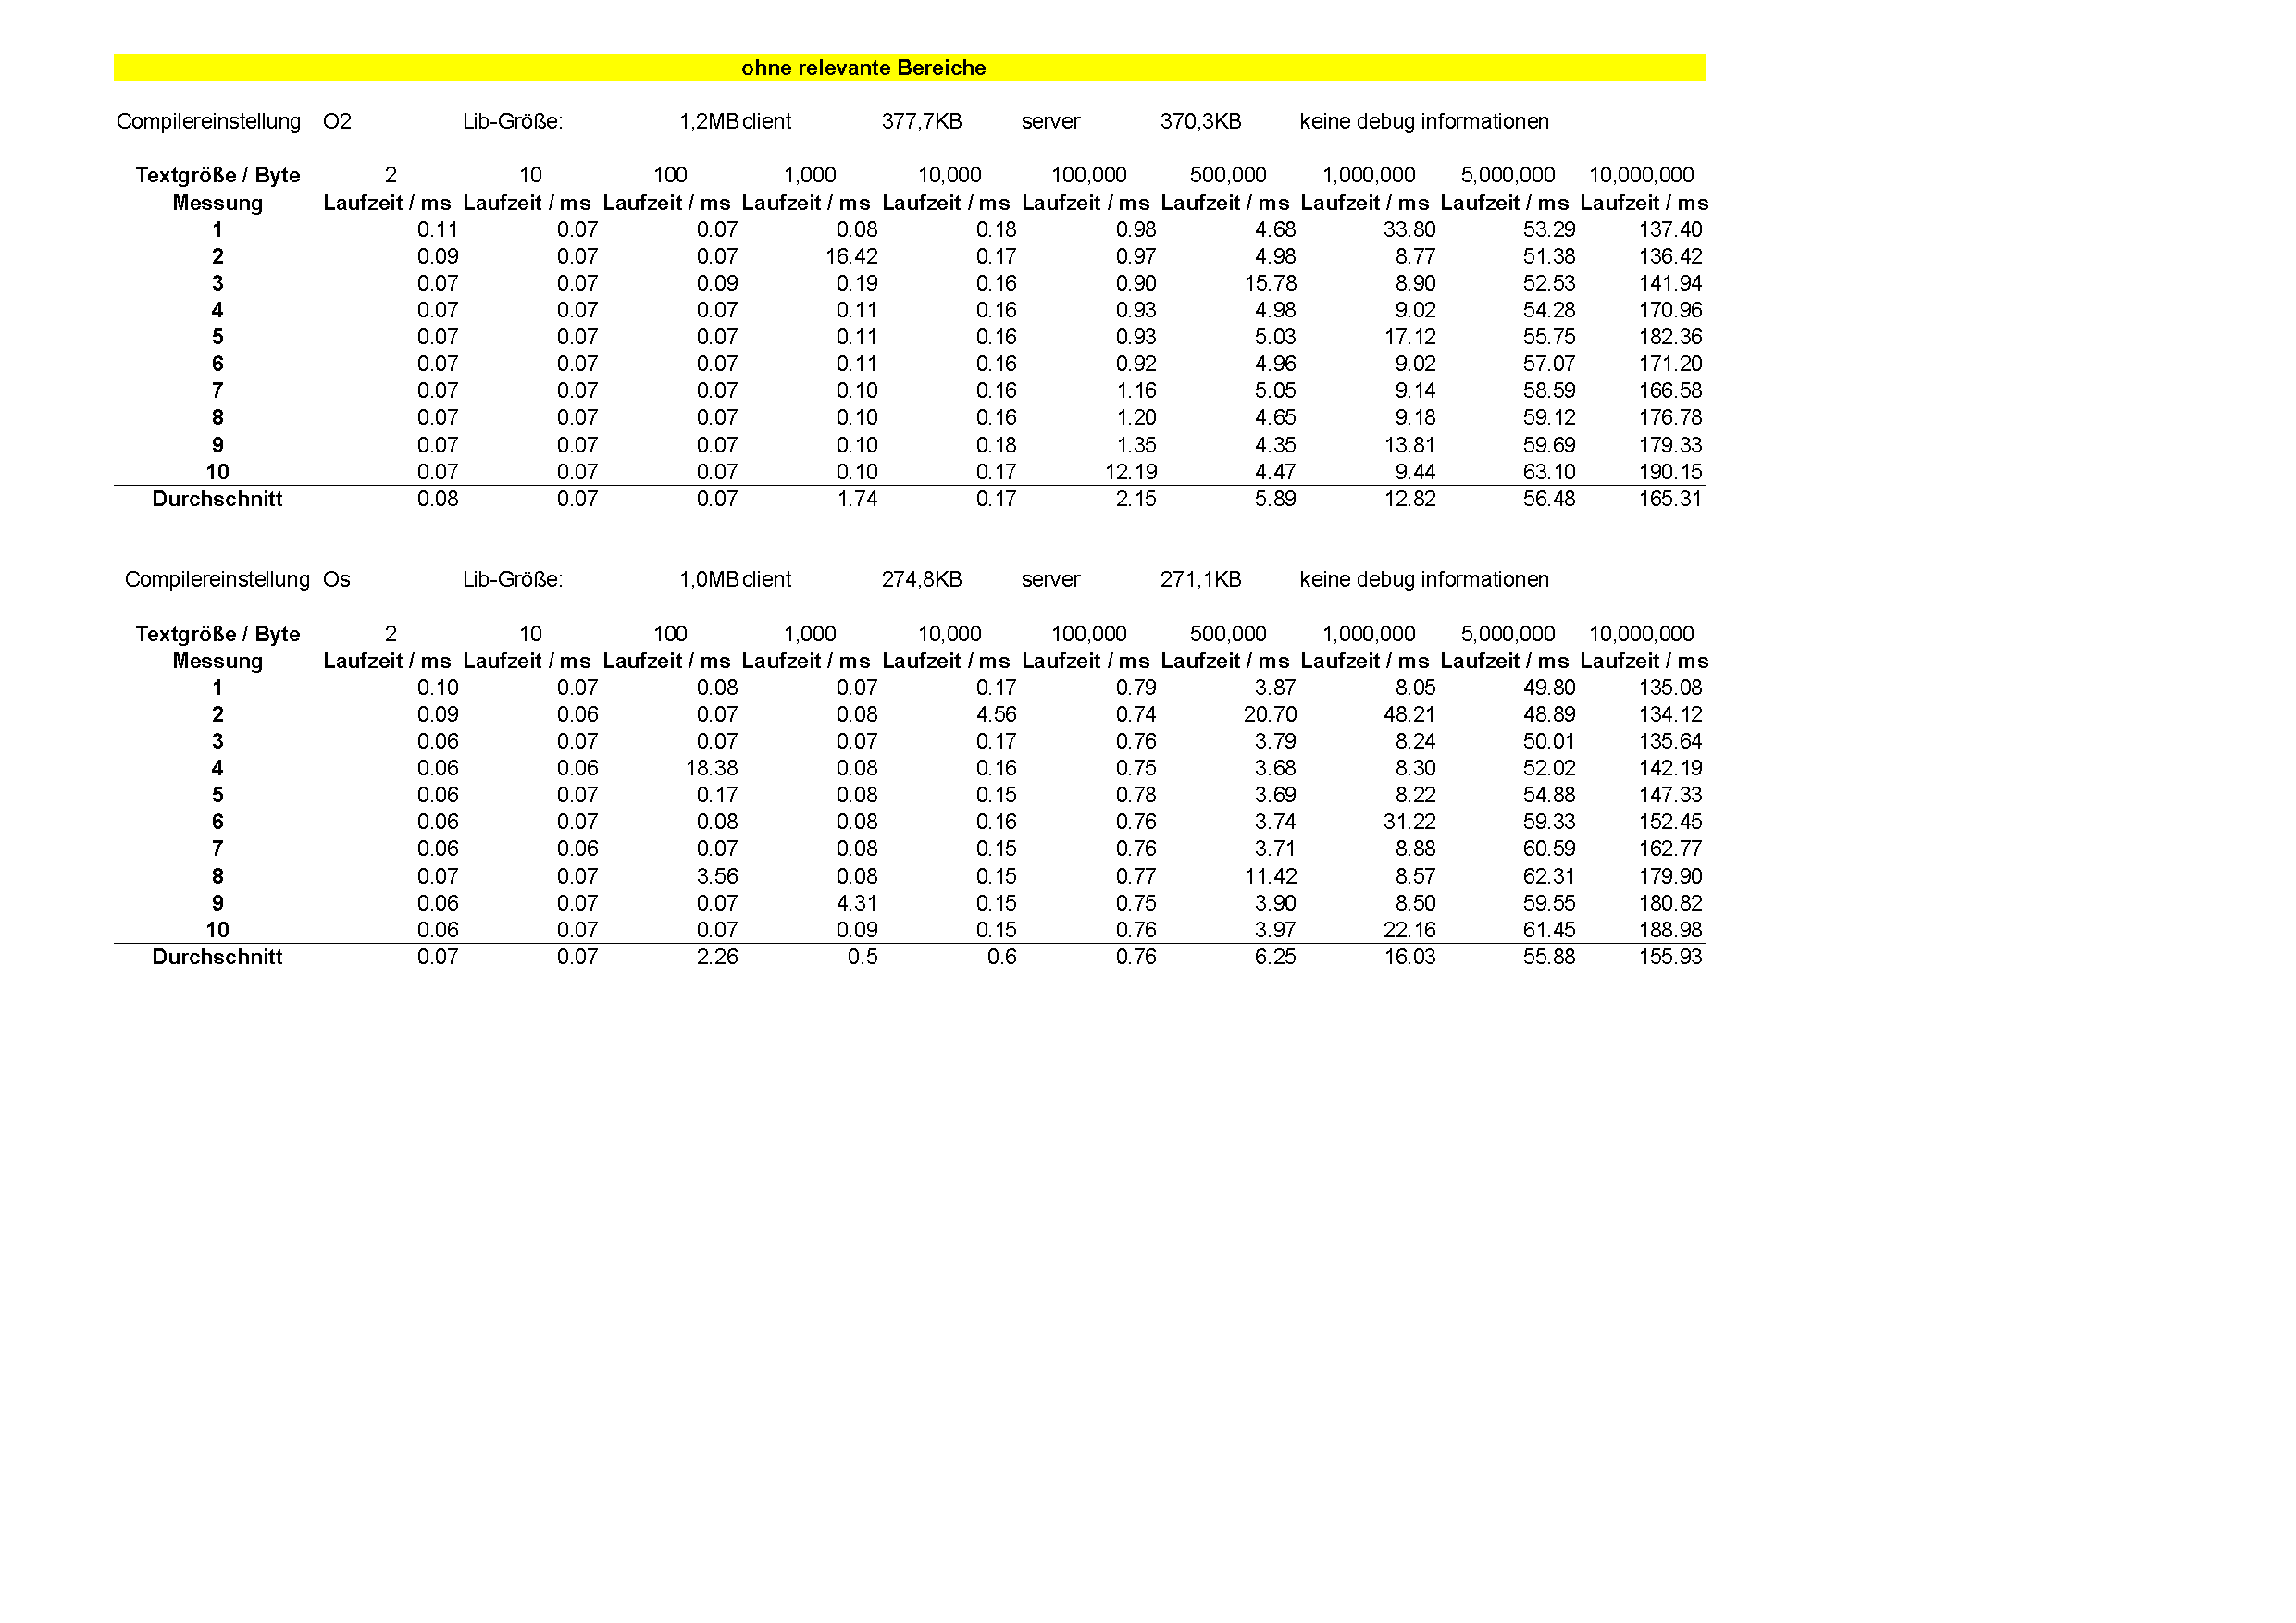
\includegraphics[angle=90,scale=.5]{MessungNormal_worp.pdf}
	\caption{Messung-Normal}	
\end{figure}

\newpage

\begin{figure}[H]
	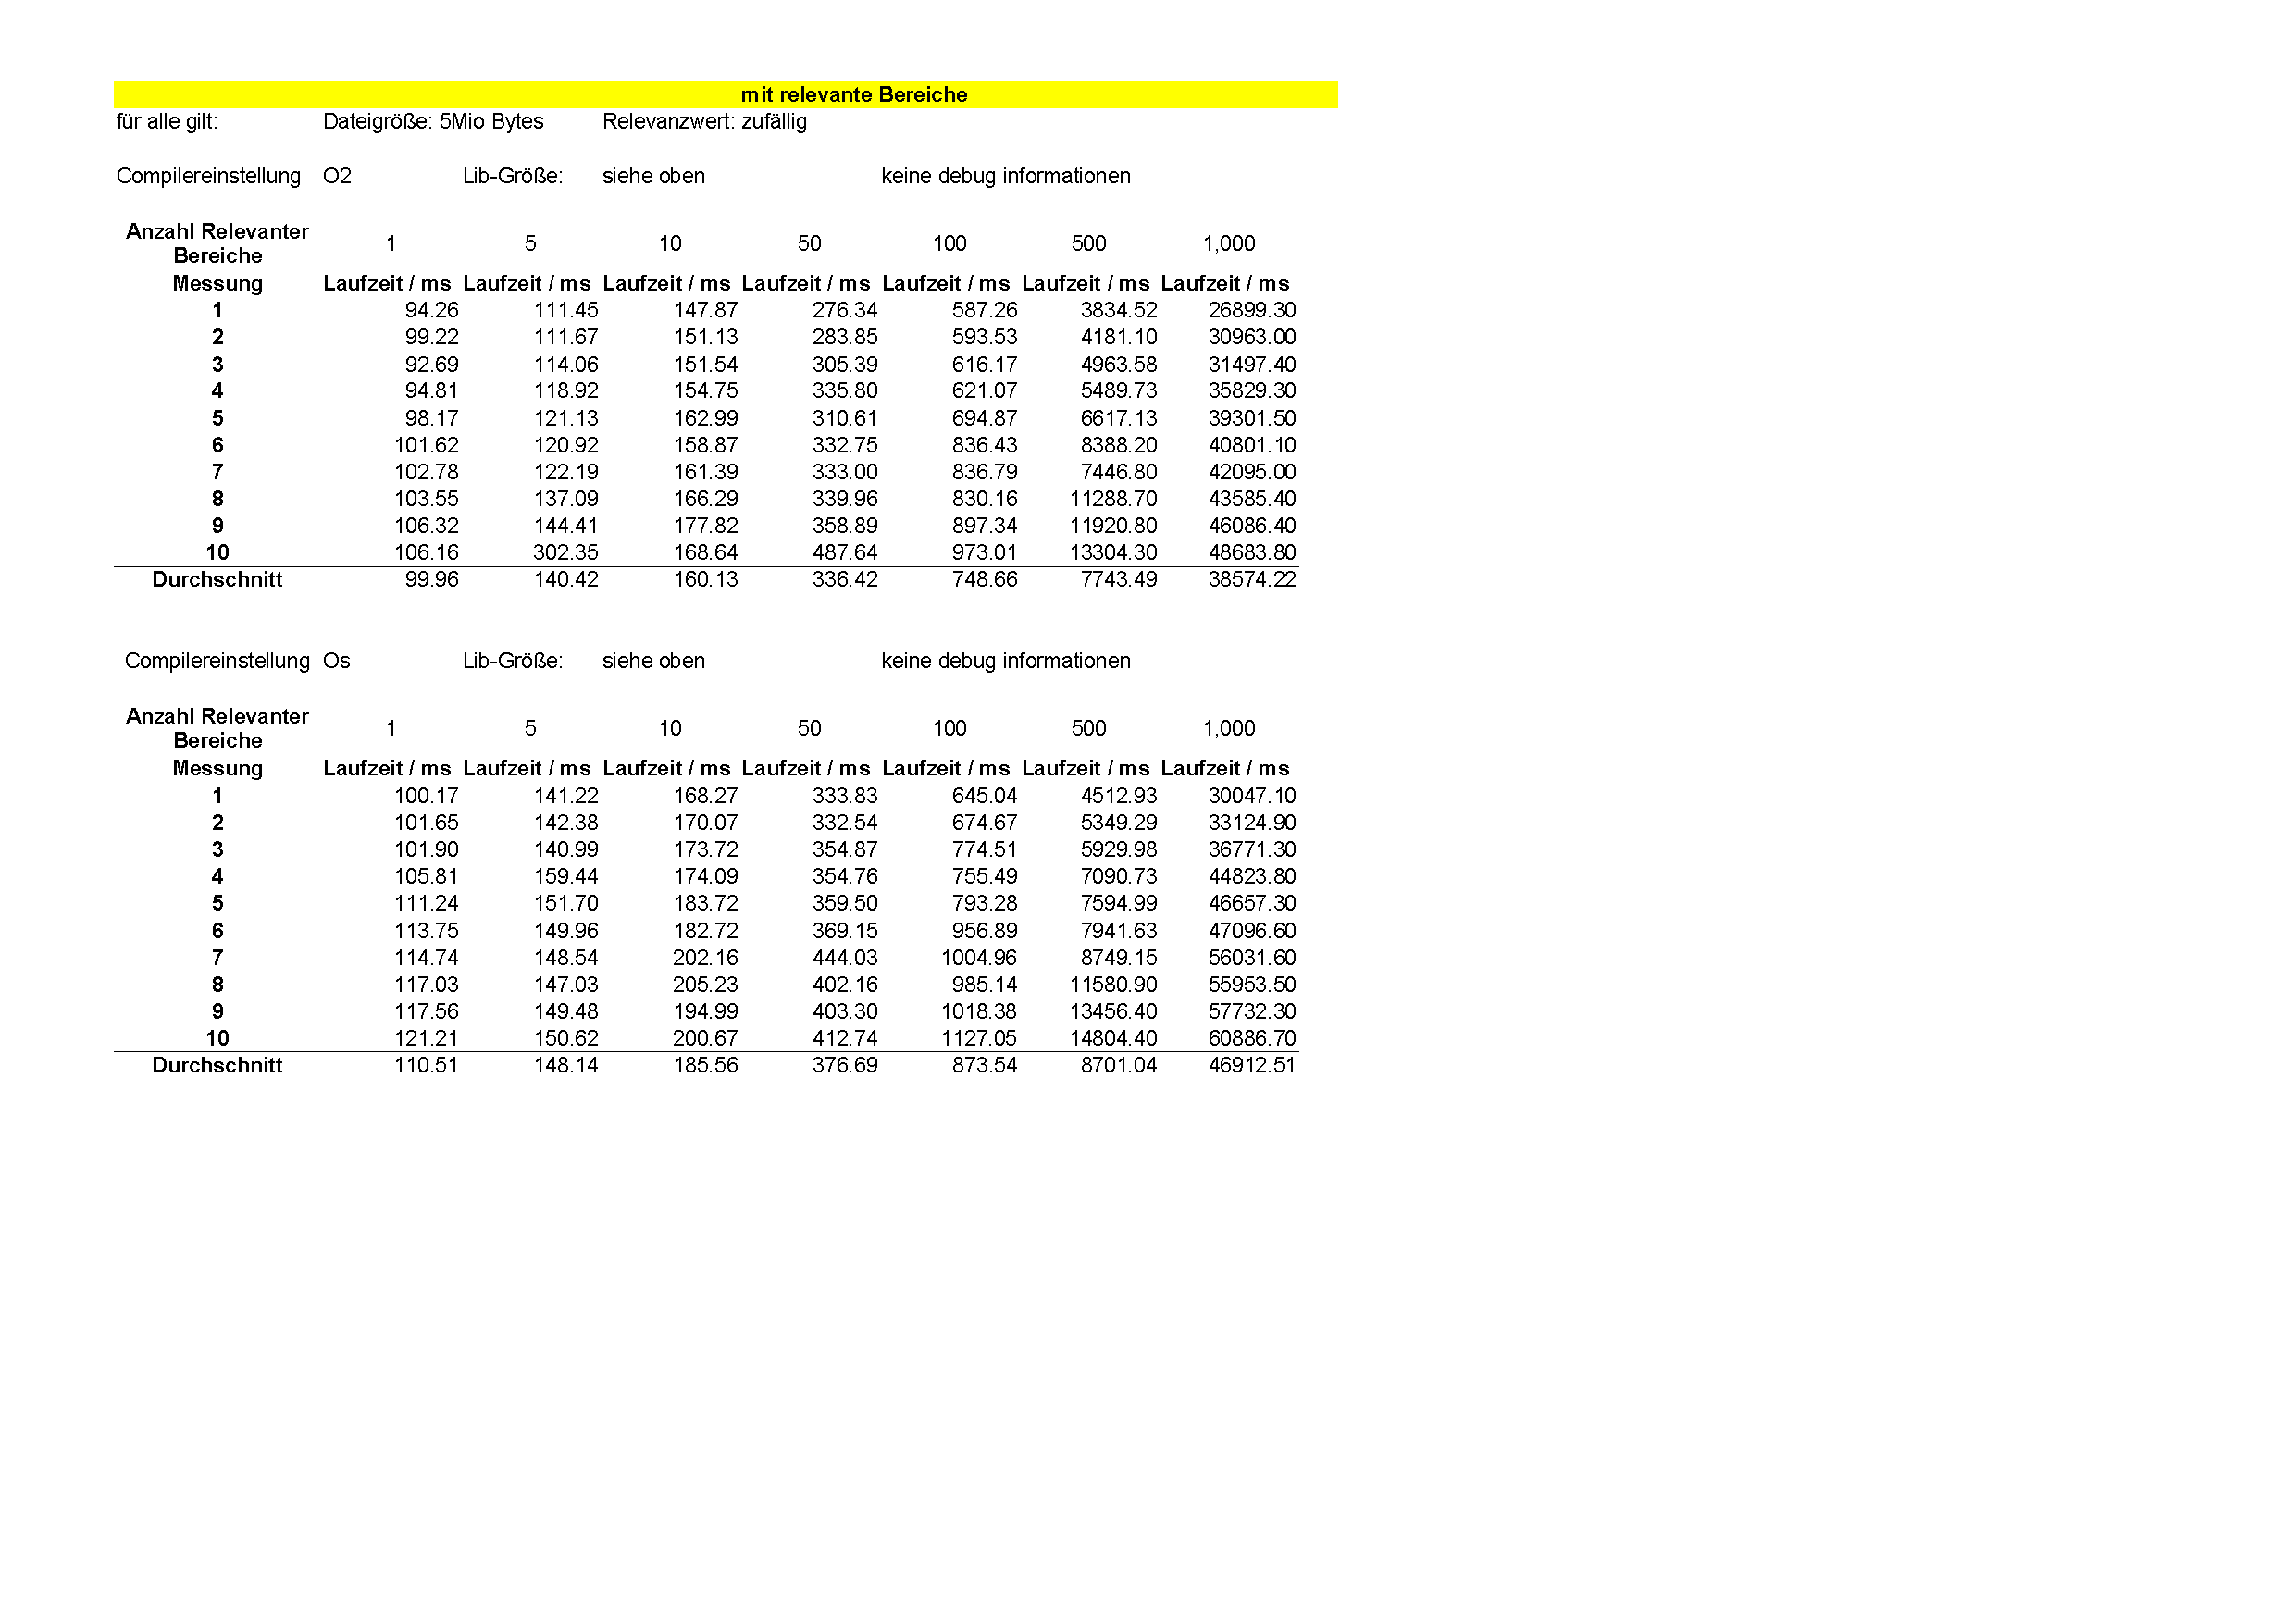
\includegraphics[angle=90,scale=.7]{MessungNormal_wrp.pdf}
	\caption{Messung-Normal}	
\end{figure}

\newpage

\begin{figure}[H]
	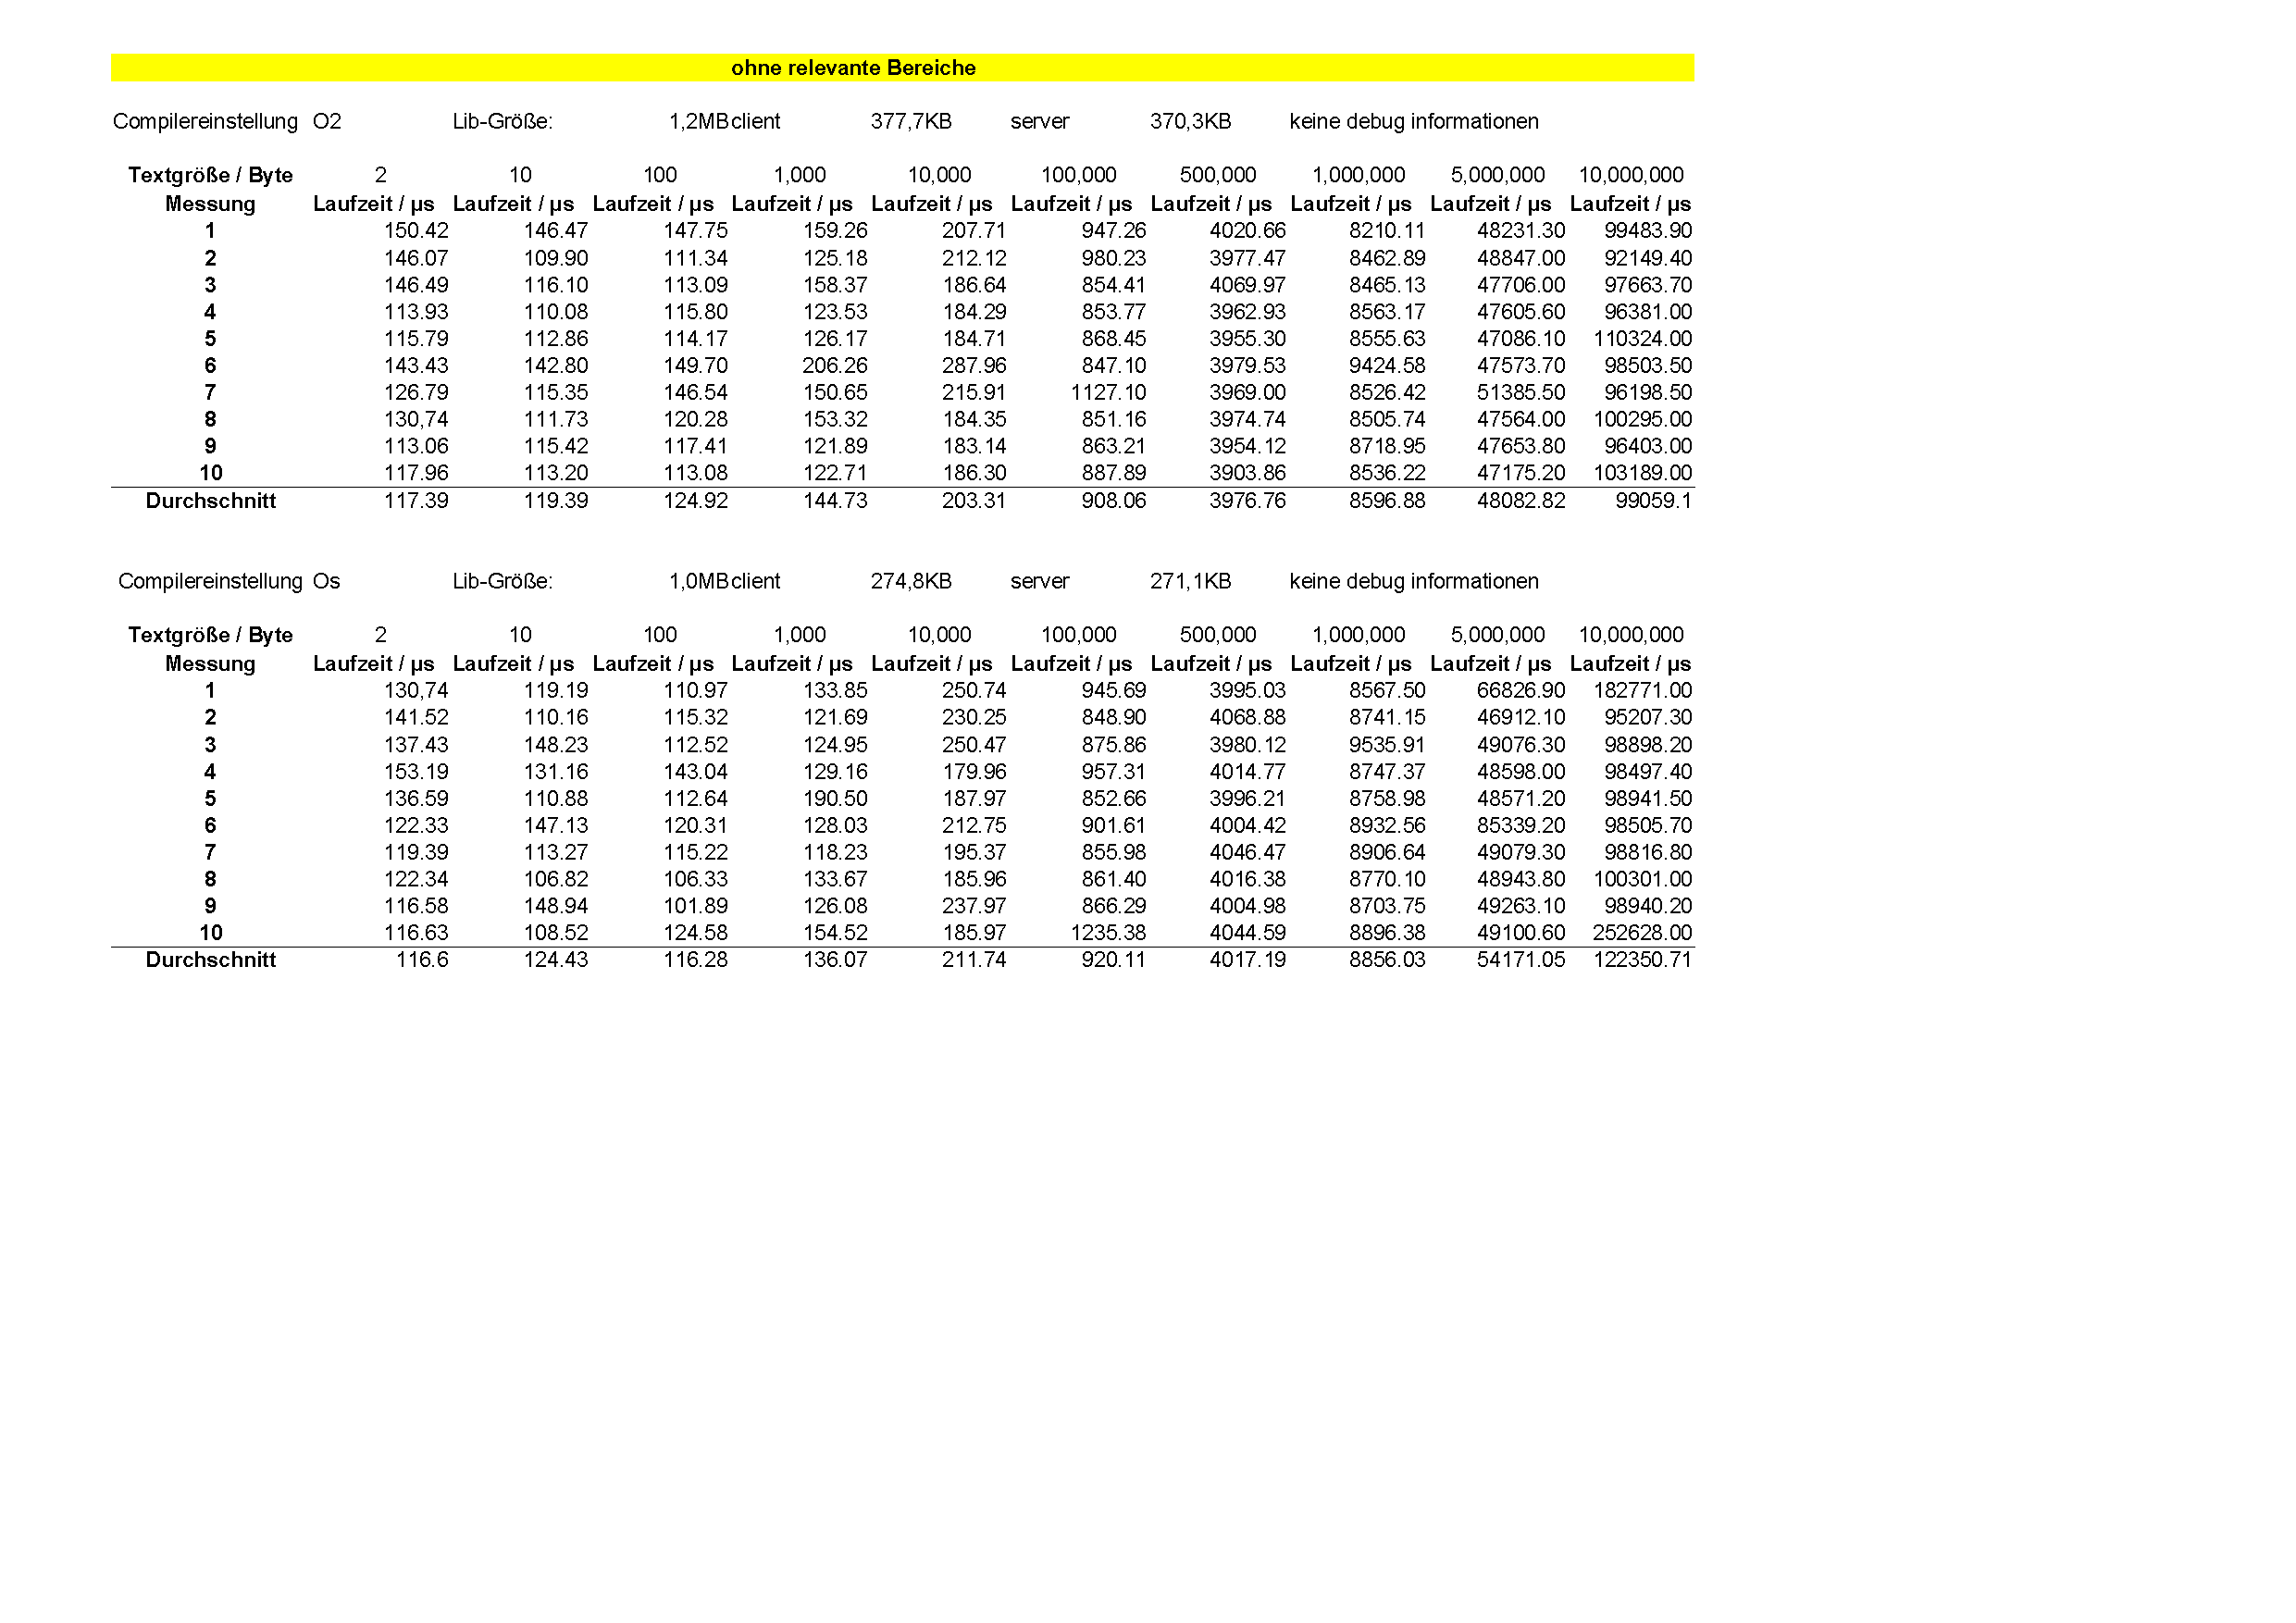
\includegraphics[angle=90,scale=.75]{MessungInitial_worp.pdf}
	\caption{Messung-Initial}	
\end{figure}

\newpage

\begin{figure}[H]
	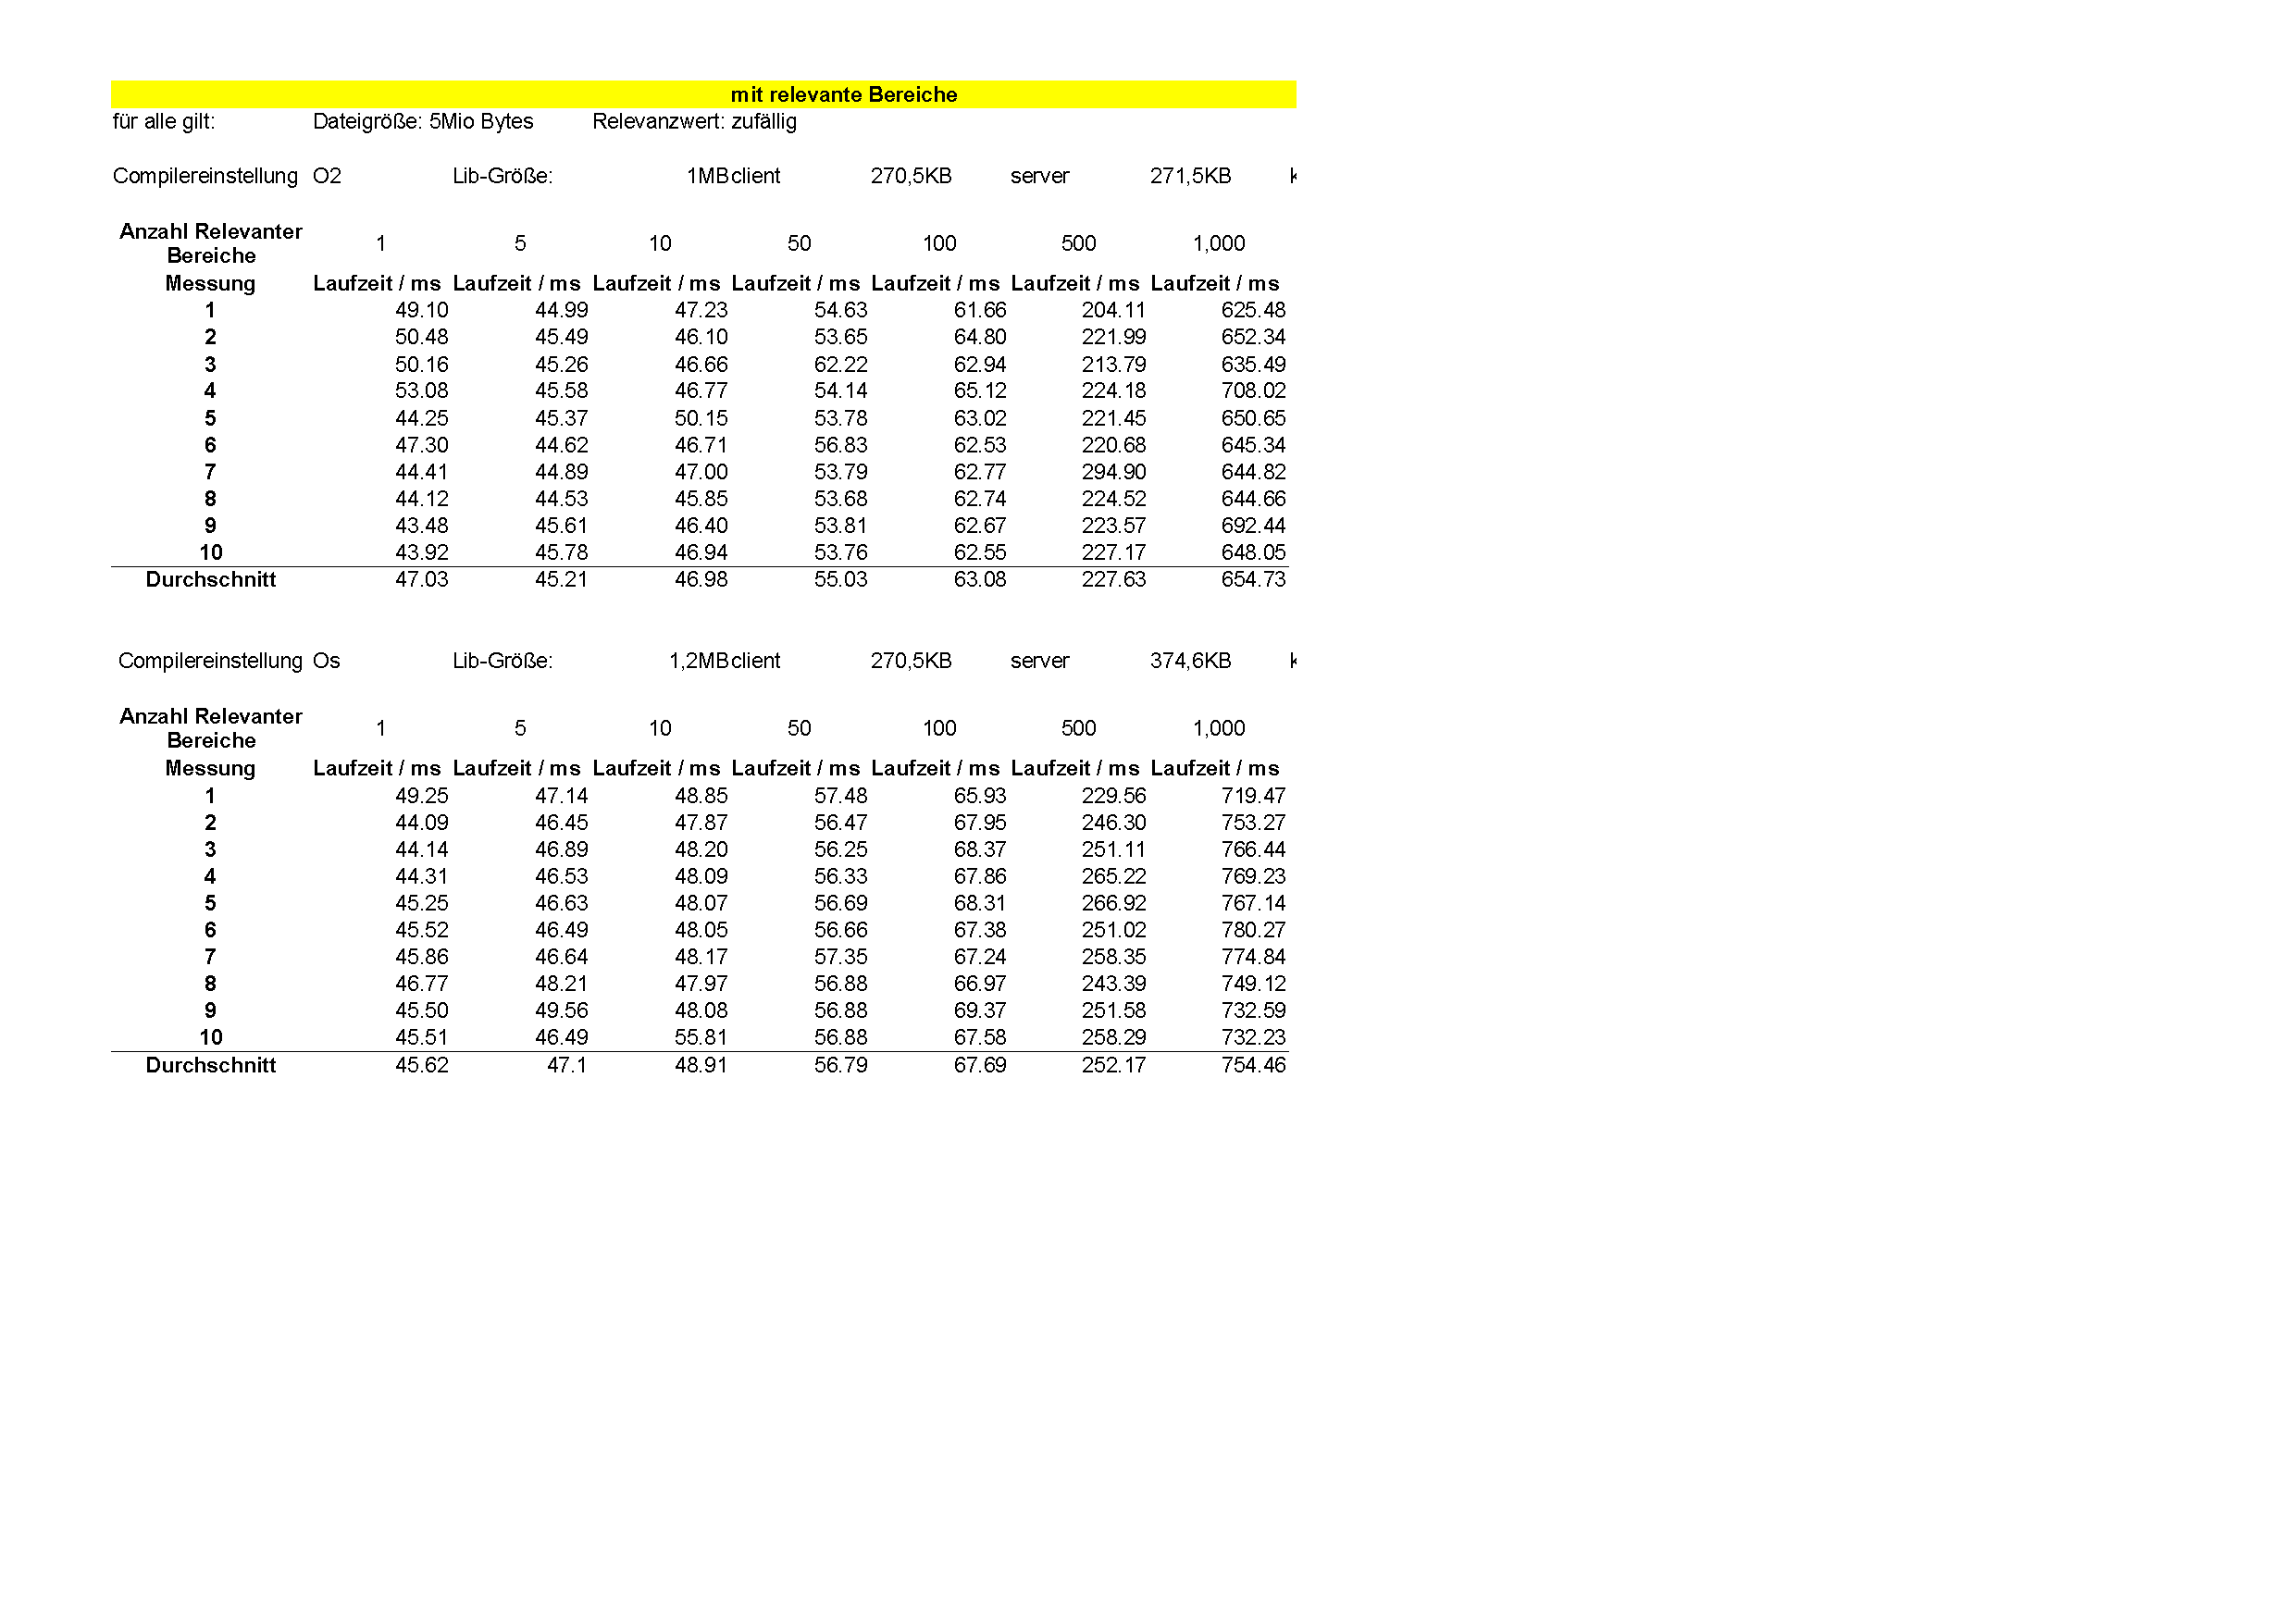
\includegraphics[angle=90,scale=.75]{MessungInitial_wrp.pdf}
	\caption{Messung-Initial}	
\end{figure}

% Die restlichen Diagramme. Müssen eventuell noch angepasst werden.
\section{Diagramme}
\label{sec:Diagramme}

\begin{figure}[H]
	\centering
	\includegraphics[angle=90,scale=.8]{DiagrammNormal_worp.pdf}
	\label{fig:diagrammNormal_worp}
	\caption{Messung-Normal ohne relevante Bereiche}
\end{figure}

\begin{figure}[H]
	\centering
	\includegraphics[angle=90,scale=.8]{DiagrammNormal_wrp.pdf}
	\label{fig:diagrammNormal_wrp}
	\caption{Messung-Normal mit relevanten Bereichen}
\end{figure}

% Größere Darstellung der Datenaufsplittung
\section{Datenaufschlüsselung}
\label{sec:Datenaufschluesselung}

\begin{figure}[H]
	\centering
	\includegraphics{DatenaufschluesselungSensor.pdf}
	\caption{Datenaufschlüsselung-Sensor}
\end{figure}

\begin{figure}[H]
	\centering
	\includegraphics{DatenaufschluesselungText.pdf}
	\caption{Datenaufschlüsselung-Text}
\end{figure}

\end{appendix}

% Index ------------------------------------------------------------------------
%   Zum Erstellen eines Index, die folgende Zeile auskommentieren.
% ------------------------------------------------------------------------------
%\printindex

\end{document}
